\documentclass[11pt,a5paper,twoside]{book}
\usepackage[utf8]{inputenc}
\usepackage[spanish]{babel}
\usepackage[T1]{fontenc}
\usepackage{lmodern}
\usepackage{microtype}
\usepackage{geometry}
\geometry{
    a5paper,
    inner=25mm,
    outer=20mm,
    top=20mm,
    bottom=20mm
}
\usepackage{graphicx}
\usepackage{titlesec}
\titleformat{\chapter}[display]
  {\normalfont\huge\bfseries\centering}{\chaptertitlename\ \thechapter}{20pt}{\Huge}
\usepackage[titles]{tocloft}
\setlength{\cftchapnumwidth}{3.5em}
\widowpenalty=10000
\clubpenalty=10000
\linespread{1.15}
\usepackage{fancyhdr}
\pagestyle{fancy}
\fancyhf{}
\fancyfoot[C]{\thepage}
\fancyfoot[R]{\rightmark}
\renewcommand{\headrulewidth}{0pt}
\renewcommand{\footrulewidth}{0pt}
\renewcommand{\thechapter}{\Roman{chapter}}
\title{Luz Vieja \\ \large Veinte años de distancia}
\author{IOREB}
\date{}

\begin{document}

\newgeometry{margin=0pt}
\thispagestyle{empty}
\noindent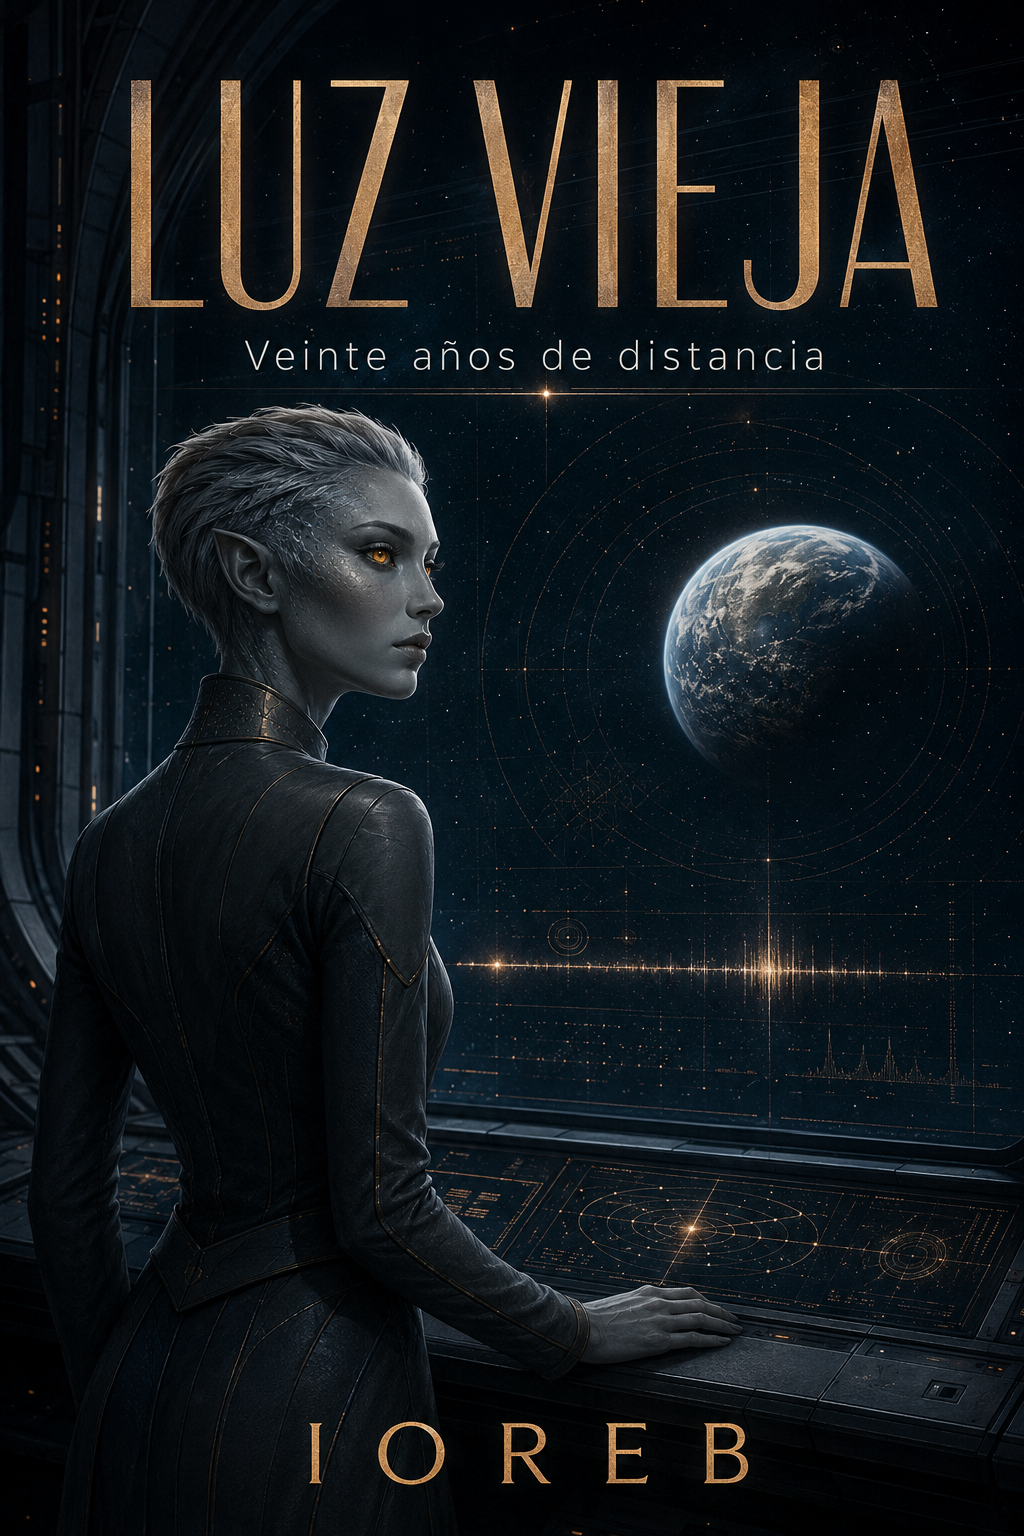
\includegraphics[width=\paperwidth, height=\paperheight]{portada.png}
\clearpage
\restoregeometry

\frontmatter
\maketitle
\clearpage
\thispagestyle{empty}
\vspace*{\fill}
\begin{center}
{\small
\textbf{Luz Vieja} \\
Autor: IOREB \\
© 2026, IOREB. Todos los derechos reservados. \\
\vspace{1.5em}
Cualquier forma de reproducción, distribución, comunicación pública o transformación de esta obra solo puede ser realizada con la autorización de sus titulares, salvo excepción prevista por la ley. Diríjase a CEDRO (Centro Español de Derechos Reprográficos) si necesita fotocopiar o escanear algún fragmento de esta obra. \\
\vspace{1.5em}
Diseño de portada: IOREB. \\
\vspace{1.5em}
Declaración de Asistencia de IA: Esta obra de ciencia ficción ha sido desarrollada y traducida con la asistencia de modelos de lenguaje de inteligencia artificial como parte de un proceso creativo agéntico iterativo en EditorIAl IOREB.
}
\end{center}
\vspace*{\fill}
\clearpage
\tableofcontents

\mainmatter
\chapter{El peso del silencio}
\markboth{El peso del silencio}{El peso del silencio}

El problema con el silencio interestelar, pensaba Seran mientras cruzaba el puente de observación, es que no es silencio en absoluto.
Era ruido. Ruido de fondo, ruido de microondas, el siseo constante del universo enfriándose desde su nacimiento. Lo que la mayoría de la gente llamaba silencio era en realidad la conversación más larga de la historia, una en la que nadie había dicho aún nada interesante. Seran llevaba diecisiete años escuchando. Hasta ahora, el universo solo había tosido.
Se detuvo frente al panel de cristal y miró hacia afuera.
La estación orbitaba a cuatrocientos kilómetros sobre Kael, el mundo que los había hecho. Desde aquí, la curvatura del planeta se mostraba sin adornos: una franja azul-verdosa de atmósfera, franjas de nubes organizadas en espirales que los modelos climáticos llevaban décadas intentando predecir sin éxito completo, y debajo de todo eso, invisible a simple vista, la red de ciudades que parpadeaba de noche como un sistema nervioso expuesto. Seran había nacido en una de esas luces. Ahora pasaba la mayor parte del tiempo aquí arriba, mirando en la dirección contraria.
Era una elección que su madre nunca había terminado de entender.
Kael giraba alrededor de una estrella naranja —Aur, la llamaban, aunque su designación técnica era un número de diecisiete dígitos que nadie usaba en conversación— a una distancia que mantenía sus océanos líquidos desde hacía algo más de cuatro mil millones de años. El planeta era más pequeño que lo que los modelos teóricos predecían como óptimo para la vida compleja, y sin embargo aquí estaban: dos mil millones de kael'thin distribuidos en doce federaciones continentales, con sus guerras, sus artes, su genómica aplicada y sus radiotelescópios apuntando hacia la nada.
Seran era una de las que apuntaban.
Aquí arriba, a cuatrocientos kilómetros de altitud, el mundo carecía de tensión. Seran sintió de nuevo ese vacío punzante en la base del cráneo, la persistencia de un miembro fantasma que buscaba un norte que ya no existía. En la superficie, el campo magnético de Kael era un anclaje invisible que ordenaba el mundo; una brújula interna constante, la certeza física de saber hacia dónde se inclinaba el planeta sin tener que pensarlo. No era un sexto sentido místico; era un río biológico integrado en su sistema nervioso, el mismo que los navegantes de la era preindustrial habían usado durante milenios para trazar rutas a través de los océanos. Aquí, en la estación, esa arquitectura interna solo devolvía un silencio sordo. En los manuales de medicina aeroespacial solía leerse que intentar describir esa privación a un kael'thin que jamás había dejado la superficie era como intentar describir un color nuevo. Una abstracción imposible. Seran, observando el parpadeo de las luces abajo, comprendió que el manual se quedaba corto: era una ceguera de orientación constante, un zumbido mudo que le recordaba a cada instante que estaba fuera de su elemento. Era lo que peor llevaba de la órbita. Eso, y la ausencia de lluvia.
Recogió su tableta de la repisa donde la había dejado y comprobó los registros nocturnos de las antenas. La Instalación Orbital de Radioastronomía Kael —IORK, para todos los que tenían que mencionarla con frecuencia— era un proyecto conjunto de ocho federaciones, lo que significaba que su financiación dependía de ocho parlamentos con ocho ciclos electorales distintos y ocho definiciones diferentes de lo que constituía un "resultado científico de interés público". Seran había aprendido a redactar informes de progreso que sonaran prometedores sin serlo, lo cual era una habilidad que la habían dicho que no necesitaría cuando estudió Astrofísica.
Los registros de la noche eran los de siempre. Pulsares. Quásares. El murmullo de fondo. Nada que no hubiera estado ahí antes.
Deslizó el dedo por las columnas de datos con la parsimonia de quien hace algo por costumbre más que por expectativa, y estaba a punto de cerrar la tableta cuando algo le hizo detenerse.
\vspace{1.5em}
\begin{center}$\ast$\quad$\ast$\quad$\ast$\end{center}
\vspace{1.5em}
La estrella era una tipo G-K, casi exactamente entre esas dos clasificaciones, a aproximadamente veinte años luz. Estaba catalogada desde hacía décadas, perfectamente ordinaria: masa ligeramente inferior a Aur, luminosidad algo menor, un sistema planetario que los espectroscopistas habían confirmado hacía ocho años mediante el método de velocidades radiales. Cuatro planetas detectados, uno de ellos en zona habitable. Nada especial. El catálogo estaba lleno de estrellas así.
Lo que no estaba en el catálogo era lo que Seran tenía ahora en la pantalla.
El perfil de emisión de radio de esa estrella era incorrecto.
No de forma dramática. No había ninguna señal pulsante con un mensaje en código morse. Era más sutil que eso, y precisamente por eso Seran llevaba diez minutos mirándolo con la sensación de que estaba viendo algo que no debería existir: en el rango de frecuencias entre 40 y 1500 megahercios, el espectro de radio de la estrella tenía picos. Picos discretos, estructurados, distribuidos de una manera que los procesos astrofísicos conocidos no producían. Las estrellas emitían radio de forma continua y suave, siguiendo distribuciones espectrales que los físicos llevaban cien años modelando con precisión. Esto no era continuo ni suave. Esto tenía forma. Tenía estructura interna.
Seran aplicó todos los filtros de artefactos de interferencia que tenía disponibles. Los picos seguían ahí.
Comprobó si algún objeto de fondo conocido —un púlsar lejano, un núcleo galáctico activo— podía estar alineado con esa dirección y produciendo la señal. Nada en el catálogo.
Los picos no eran periódicos entre sí de ninguna forma simple, lo cual descartaba un solo objeto rotante como fuente. Eran más bien una superposición de múltiples emisores: algo que producía radio en varias frecuencias simultáneamente, con intensidades que variaban de forma independiente. Era casi como... ruido estructurado. Ruido que había sido modulado por algo antes de emitirse.
Seran permaneció quieta frente al panel de cristal durante un largo rato. Afuera, Kael seguía girando con su indiferencia habitual.
"Probablemente sea interferencia de algún satélite nuestro", pensó, forzando la hipótesis más aburrida. Siempre primero la más aburrida.
Pero los satélites de la IORK tenían frecuencias registradas, y ninguna coincidía con los picos que estaba viendo.
Etiquetó la entrada en el registro con prioridad máxima de análisis. No alertó a nadie todavía.
Luego cerró la tableta. Luego la volvió a abrir.

\chapter{La curvatura del tiempo perdido}
\markboth{La curvatura del tiempo perdido}{La curvatura del tiempo perdido}

El Instituto de Física Teórica de Kael Septentrional ocupaba un edificio que había sido diseñado en una época en que los arquitectos todavía creían que la forma debía comunicar el contenido. Era una estructura baja y horizontal, construida en piedra gris del delta, con ventanas largas y estrechas que dejaban entrar la luz de Aur en ángulos calculados para que los despachos nunca estuvieran del todo en sombra ni del todo iluminados. Alguien con mucho tiempo y cierta tendencia a la interpretación simbólica podría haber dicho que el edificio parecía un objeto en el límite entre dos estados. Los físicos que trabajaban dentro solían decir simplemente que en invierno hacía frío.
Tael llegó esa mañana con veinte minutos de adelanto, lo cual era inusual incluso para él.
Había dormido mal. No por ansiedad, o no exactamente: era más bien la sensación de tener algo en la cabeza que no cabía del todo, como intentar cerrar una caja cuya tapa no encaja porque hay demasiado dentro. Los últimos tres años del proyecto habían sido una secuencia de aproximaciones sucesivas a un resultado que siempre parecía estar a dos pasos, y ahora, de repente, la simulación de la semana anterior había devuelto números que cuadraban. No aproximadamente. Exactamente.
Tael era suficientemente buen físico como para desconfiar de los resultados exactos.
Colgó su abrigo —hacía frío, como siempre en invierno— y encendió la terminal antes de quitarse la bufanda. Los archivos de la simulación seguían abiertos donde los había dejado la noche anterior. Los miró con el estatismo denso de quien espera encontrar el error que sabe que tiene que estar ahí en algún lado.
Los números seguían cuadrando.
\vspace{1.5em}
\begin{center}$\ast$\quad$\ast$\quad$\ast$\end{center}
\vspace{1.5em}
El proyecto tenía un nombre oficial largo que nadie usaba y un nombre informal que todo el mundo usaba: La Burbuja. Había empezado, como muchos proyectos de física teórica, como una consecuencia no buscada de otra investigación. Hacía doce años, un equipo de Kael Meridional había estado estudiando las propiedades de la métrica espacio-temporal en presencia de densidades de energía negativa —un campo oscuro y técnico que en ese momento parecía interesante principalmente para los especialistas en relatividad general y para nadie más— cuando uno de sus miembros, casi de pasada, había publicado un paper calculando el coste energético de crear una deformación local del espacio lo suficientemente pequeña como para que no contuviera materia.
El paper había recibido pocas citas al principio. Luego, gradualmente, había empezado a acumularlas.
El problema con mover materia mediante deformación métrica era energético y además fundamental: la cantidad de energía negativa necesaria para crear y estabilizar una burbuja del tamaño suficiente para contener incluso un gramo de materia era astronómica en el sentido más literal, y además existían objeciones de causalidad que los teóricos llevaban décadas intentando resolver sin éxito claro. Pero el paper de Kael Meridional había identificado algo distinto: una solución de escala mínima. Una burbuja tan pequeña que no pudiera contener nada con masa en reposo. Una burbuja que no pudiera transportar materia.
Pero que sí podía transportar un estado.
La diferencia era sutil y llevaba años explicarla bien a quien no era físico, pero la idea central era esta: la información no era materia. Un bit —un estado, un sí o un no— no pesaba nada. Y si podías crear una burbuja de deformación métrica lo suficientemente pequeña y estable, la burbuja podía propagarse a través del espacio transportando ese estado sin violar ninguna ley de conservación relevante, porque no había nada dentro que conservar. La burbuja no movía materia. Movía geometría.
Y la geometría podía moverse más rápido que la luz.
Los problemas eran, naturalmente, numerosos.
El primero era energético: incluso a esa escala mínima, el coste por bit enviado era enorme comparado con cualquier sistema de comunicación convencional. No prohibitivo —la fusión comercial daba para mucho—, pero sí lo suficientemente alto como para que nadie pensara en usar esto para sustituir la red de comunicaciones planetaria. Era una tecnología de un único caso de uso obvio: mandar información a distancias donde la velocidad de la luz se convierte en un problema real.
El segundo era de coherencia: la burbuja tendía a deformarse durante la propagación, lo que corrompía el estado que transportaba. Era como mandar una carta dentro de un sobre que se mojaba durante el viaje. Los tres años del proyecto de Tael habían sido, en esencia, el problema de encontrar cómo impermeabilizar el sobre.
Y la simulación de la semana anterior decía que lo habían conseguido.
\vspace{1.5em}
\begin{center}$\ast$\quad$\ast$\quad$\ast$\end{center}
\vspace{1.5em}
Milen llegó a las horas de siempre, que era decir tarde, con un contenedor térmico en cada mano y esa postura ligeramente ladeada de quien ya intuye que hay novedades.
Milen era la codirectora del proyecto, física experimental frente al perfil teórico de Tael, y llevaban suficientes años trabajando juntos como para tener un idioma propio hecho de silencios y de qué tipo de pausa hacía cada uno antes de hablar.
—Siguen cuadrando —dijo Tael sin moverse de la pantalla.
Milen dejó una de las tazas sobre su mesa con el cuidado de quien no quiere celebrar demasiado pronto.
—¿Has encontrado el error?
—He buscado durante dos horas.
—¿Y?
—No está.
Milen se sentó en la silla que había frente a su terminal —no su silla, pero llevaba años sentándose ahí con suficiente frecuencia como para que tuviera la forma de ella— y miró los números.
—El término de corrección de fase funciona —dijo, en voz baja. No era una pregunta.
—El término de corrección de fase funciona. —Tael se echó hacia atrás—. La coherencia de la burbuja se mantiene por encima del noventa y cuatro por ciento en toda la propagación hasta los límites del modelo. Con esa tasa de fidelidad, los protocolos de corrección de errores estándar pueden recuperar el estado original sin degradación detectable.
Milen no dijo nada durante un momento.
La ventana larga y estrecha que tenía delante dejaba entrar la luz de Aur, que esa mañana era del color del cobre viejo. Fuera, el delta del río que rodeaba el instituto estaba cubierto de una niebla baja que se disolvía lentamente con el calor de la mañana. Dos aves grandes planeaban en círculos sobre el agua.
—Cuánto —dijo por fin.
—El modelo escala hasta tres años luz con los parámetros actuales antes de que la degradación empiece a superar el umbral de corrección. Con mejoras en el generador de contención, posiblemente diez.
—¿Y el coste energético por bit?
—A distancias interestelares, aproximadamente el equivalente a lo que consume una ciudad mediana durante un segundo por cada diez bits transmitidos.
Milen sopesó la cifra.
—Es caro.
—Es absurdamente caro para cualquier comunicación ordinaria. Para una comunicación interestelar, es irrelevante. Si alguna vez hay algo a lo que querer mandar un mensaje a varios años luz de distancia, el coste energético no va a ser el factor limitante.
—Si alguna vez hay algo —repitió Milen.
Era la condición que nadie mencionaba en los papers. El proyecto tenía un nombre y tenía financiación y tenía sentido como investigación fundamental, pero todos en el equipo eran suficientemente adultos como para saber que estaban construyendo una tecnología para una conversación que quizás no tendría lugar nunca. Mandar información más rápido que la luz solo importaba si había alguien al otro lado que quisiera recibirla.
Y hasta ese momento, el universo no había dado indicios de que hubiera nadie.
—Necesitamos construir el prototipo físico —dijo Tael—. La simulación no basta. Tenemos que demostrarlo en un experimento real, aunque sea a escala de laboratorio, aunque sea a un metro de distancia.
—Eso es presupuesto nuevo.
—Sí.
—¿Cuánto?
Tael le pasó una hoja con los cálculos. Milen la leyó. Sostuvo la mirada el tiempo exacto que Tael había aprendido a decodificar como: \textit{más de lo que tenemos pero menos de lo que temía}.
—Voy a llamar al comité de financiación esta tarde —dijo Milen, levantándose—. Necesito que me prepares un resumen ejecutivo que no use la expresión "densidad de energía negativa" en las primeras dos páginas.
—Es un término técnico necesario.
—Es un término que hace que los parlamentarios piensen en magia. Dos páginas, Tael. Luego puedes poner toda la densidad de energía negativa que quieras.
Tael dejó caer el peso de su cuerpo hacia atrás, evaluando si valía la pena objetar antes de decidir que no.
—Dos páginas —dijo.
Milen ya estaba en la puerta cuando se giró.
—Tael. —Una pausa—. Si esto funciona en el prototipo... ¿cuánto tiempo hasta un sistema operativo real? No el modelo óptimo. El primero que sirva para algo.
Tael pensó. Era el tipo de pregunta que prefería no responder sin los números delante, pero conocía los números de memoria.
—Cuatro años. Quizás cinco, si la ingeniería del generador es difícil.
Milen encajó el dato en silencio, con la tensión de alguien que está haciendo una aritmética que no tiene que ver con la física.
—Bien —dijo, y se fue.
Tael se quedó mirando la puerta cerrada un momento. Luego volvió a la pantalla.
Los números seguían cuadrando.
\vspace{1.5em}
\begin{center}$\ast$\quad$\ast$\quad$\ast$\end{center}
\vspace{1.5em}
Aquella misma noche, a cuatrocientos kilómetros sobre el planeta, Seran estaba en la sala de control de la IORK mirando los primeros datos de la sesión de seguimiento.
La anomalía seguía ahí.
Con cuarenta y ocho horas adicionales de tiempo de integración, el perfil era ahora más nítido, y más nítido significaba más imposible de explicar con tranquilidad. Los picos espectrales en el rango de radio no solo se confirmaban: mostraban una subestructura que los datos de la primera noche no habían tenido resolución suficiente para revelar. Había patrones dentro de los patrones. Modulaciones. La señal no era una sola fuente puntual sino algo distribuido —múltiples emisores superpuestos— y la distribución de frecuencias tenía una forma que Seran había estado describiendo en sus notas como no térmica con estructura compleja, que era su manera de escribir lo que todavía no se atrevía a escribir con otras palabras.
Abrió el catálogo de interferencias conocidas por cuarta vez y lo recorrió por cuarta vez sin encontrar nada.
Luego hizo algo que llevaba dos días evitando hacer: buscó en la literatura de SETI, el programa de búsqueda de inteligencia extraterrestre que los kael'thin llevaban ochenta años financiando con entusiasmo variable. Buscó específicamente en los papers sobre firmas de radio de civilizaciones tecnológicas. Lo que describían como señal artificial detectable.
Los papers describían exactamente lo que ella estaba viendo.
Seran cerró la búsqueda. Se quedó mirando la pantalla en blanco durante un minuto.
Luego la reabrió y siguió leyendo.

\chapter{Objetos sin clasificar}
\markboth{Objetos sin clasificar}{Objetos sin clasificar}

La semana de observación se convirtió en tres semanas sin que nadie lo decidiera formalmente.
Así funcionaban estas cosas: Orath había dicho una semana y al final de esa semana los datos eran suficientemente extraños como para que nadie en la sala de revisión propusiera detener las observaciones, y como nadie lo propuso, las antenas siguieron apuntando, y los datos siguieron acumulándose, y la semana se convirtió en dos y luego en tres con la misma lógica silenciosa con que una conversación interesante se extiende más allá de la hora en que todos habían planeado irse a dormir.
Seran había reorganizado su rutina sin darse cuenta de que lo estaba haciendo. Dormía menos. Comía en la sala de control con más frecuencia que en el comedor. Tenía tres cuadernos abiertos simultáneamente en su mesa, y los tres tenían la misma característica: las primeras páginas eran ordenadas, con hipótesis numeradas y datos citados con precisión, y las páginas más recientes eran una conversación consigo misma que se había ido volviendo progresivamente menos ordenada a medida que los datos se negaban a resolverse en algo simple.
La señal —ya la llamaban la señal, en la sala de control, sin mayúsculas pero con el peso específico que tienen las palabras cuando se usan para referirse a algo que no tiene nombre todavía— era real.
Esto ya no era una hipótesis. Era una conclusión.
Preva había sido la primera en decirlo en voz alta, en la segunda semana, con el tono plano de quien anuncia un resultado de laboratorio sin querer que el tono añada información que los datos todavía no justifican: el espectro de radio de esa estrella no es consistente con ningún modelo de emisión estelar en el catálogo, ni con variaciones de parámetros dentro de rangos físicamente plausibles. No es ruido natural. Y luego había guardado silencio, porque lo que seguía a esa conclusión era algo que nadie quería ser el primero en escribir en un documento oficial.
Los datos de la tercera semana habían añadido la segunda pieza.
Seran había coordinado con los satélites de observación infrarroja para apuntar en la misma dirección. Lo que buscaba era el exceso de emisión térmica: una biósfera activa, una civilización industrial, ambas cosas generan calor residual que se escapa al espacio en longitudes de onda infrarrojas. Era una firma débil a veinte años luz, al límite de lo detectable con los instrumentos disponibles, pero los datos devolvieron un exceso claro. El planeta —el tercero del sistema, el que estaba en zona habitable— emitía más calor del que podía explicarse por el equilibrio radiativo con su estrella.
No mucho más. Pero sí más.
El tipo de más que produce un planeta con océanos, con continentes, con una atmósfera que trabaja. Con vida.
Y luego llegó la tercera pieza, la que Seran había estado esperando sin admitir que la esperaba.
El planeta rotaba. Y mientras rotaba, la intensidad de la señal de radio variaba con un período de aproximadamente setenta y un horas —el día sidéreo del planeta, calculó Seran, aunque no podía confirmarlo sin más datos— con una asimetría clara: había un hemisferio que emitía más que el otro. No mucho más. Pero sí de forma consistente, sesión tras sesión, con la regularidad de algo que era una propiedad estructural del objeto y no un fenómeno transitorio.
Un hemisferio más ruidoso que el otro.
Seran había escrito en su cuaderno, con letra muy pequeña, las dos palabras que explicaban eso. Luego había pasado la página.
\vspace{1.5em}
\begin{center}$\ast$\quad$\ast$\quad$\ast$\end{center}
\vspace{1.5em}
La reunión de la tercera semana fue diferente a las anteriores.
Las primeras dos habían tenido el tono de una revisión científica ordinaria: presentación de datos, discusión de hipótesis, acción a seguir. Esta tenía algo distinto en el aire desde el momento en que Seran entró en la sala. Era algo en la forma en que la gente ocupaba sus sillas —demasiado quietos, demasiado conscientes de sus propios movimientos— y en que las conversaciones previas al inicio se cortaron antes de lo habitual.
Orath estaba al fondo de la sala, de pie, en estricto alineamiento vertical. Era su postura de \textit{esto es importante, lo sé, y prefiero minimizar mi huella térmica}.
Seran presentó los datos en orden. La anomalía espectral inicial. Las cuarenta y ocho horas de seguimiento. La confirmación del exceso infrarrojo. La variabilidad rotacional con asimetría hemisférica. Lo hizo sin dramatizar, porque los datos no necesitaban dramatización y porque en su experiencia la dramatización en ciencia producía dos reacciones igualmente inútiles: o el oyente se dejaba llevar por el entusiasmo y dejaba de pensar críticamente, o se ponía en guardia contra lo que percibía como exageración y empezaba a buscar errores con más energía de la necesaria.
Cuando terminó, hubo silencio.
Fue Colm quien habló primero.
—¿Cuál es la hipótesis que mejor se ajusta a todos los datos simultáneamente? —preguntó—. No la más probable. La que mejor ajusta.
Seran no necesitó pensarlo.
—Una civilización tecnológica en el planeta habitable del sistema —dijo—. Con fuentes de emisión de radio distribuidas de forma no uniforme sobre la superficie. Suficientemente desarrollada para generar un exceso de calor residual detectable a veinte años luz. Cuya burbuja de contaminación electromagnética se expande a la velocidad de la luz y alcanza nuestra posición.
La sala absorbió la información en silencio.
—¿Cuánto tiempo lleva esa burbuja viajando? —preguntó Verath.
—Veinte años, si la fuente está a veinte años luz. Lo que estamos viendo ahora es lo que emitían hace dos décadas.
—Así que podrían ser más avanzados ahora.
—Sí. O podrían no existir ya. Lo que detectamos es luz vieja. Una fotografía del pasado.
—¿Podría ser natural? —preguntó Rannek, el ingeniero de sistemas, que había estado callado hasta ese momento—. ¿Algún mecanismo que no hayamos considerado?
—He pasado semanas buscándolo —dijo Seran—. El espectro de radio no es reproducible por ningún proceso astrofísico conocido. El exceso infrarrojo en combinación con esa firma espectral no tiene análogo natural en el catálogo. Y la asimetría hemisférica que rota con el planeta... —hizo una pausa— eso solo lo produce algo en la superficie del planeta que no está distribuido uniformemente. La naturaleza puede ser muchas cosas, pero no construye transmisores de radio que cubren preferentemente un hemisferio.
Nadie respondió a eso.
—Necesitamos el espectro atmosférico —dijo Orath desde el fondo.
—Lo sé. Es el siguiente paso. Si conseguimos una observación espectroscópica directa del planeta durante un tránsito, podemos analizar la composición de su atmósfera. —Seran había preparado esta parte—. Si hay oxígeno libre y metano en proporciones que no pueden mantenerse en equilibrio sin una fuente continua, es una biósfera activa. Si además hay óxido nitroso u otros compuestos que solo produce la industria, es una biósfera con química artificial. —Una pausa—. El próximo tránsito calculado del planeta frente a su estrella es en treinta y ocho días. Necesito coordinar tiempo en los telescopios espaciales de alta apertura.
—Lo tienes —dijo Orath. Sin deliberar, sin condiciones. Seran llevaba suficiente tiempo en la IORK como para saber que eso era inusual—. Y necesito que alguien empiece a pensar en el protocolo. Si la espectroscopía confirma lo que estamos viendo, esto deja de ser una anomalía de investigación interna.
Nadie preguntó qué protocolo. Todos sabían a qué se refería: las ocho federaciones que financiaban la IORK, sus parlamentos, sus ministerios de ciencia, y detrás de todo eso, la estructura política de un planeta que nunca había tenido que tomar una decisión de este tipo.
La reunión terminó con la sensación específica de que algo había cambiado de categoría.
\vspace{1.5em}
\begin{center}$\ast$\quad$\ast$\quad$\ast$\end{center}
\vspace{1.5em}
Seran tardó en irse.
Dovat se quedó también. Era su hábito: siempre el último en salir, como si la sala de control necesitara que alguien cerrara con llave aunque no hubiera llave que cerrar.
—¿Estás bien? —preguntó, cuando los demás se habían ido.
—Sí. —Una pausa—. No lo sé.
Dovat aceptó la pausa en silencio, como si la duda en sí misma fuera una respuesta completamente satisfactoria.
—Hace diecisiete años que buscas —dijo.
—Dieciocho. El año de doctorado cuenta.
—Dieciocho. —Dovat miró la pantalla donde todavía estaba abierto el espectro de radio—. ¿Qué se siente?
—Como cuando estás leyendo un libro muy largo —dijo Seran por fin— y llevas horas sin que pase nada y de repente en una página hay una frase que cambia todo lo que creías que sabías sobre lo que estabas leyendo, y tienes que parar y volver atrás y releer las páginas anteriores con ojos distintos. —Una pausa—. Pero todavía no sé si es esa frase o si me la he imaginado.
Dovat miró la pantalla un momento más.
—La espectroscopía del tránsito lo dirá —dijo.
—Sí. En treinta y ocho días.
—¿Y si confirma?
Seran cerró el último cuaderno.
—Entonces —dijo— deja de ser mi descubrimiento y empieza a ser de todos. —Una pausa más larga—. Y en algún lugar de ese sistema hay algo que lleva décadas enviando señales sin saber que alguien las está recibiendo.
Dovat no dijo nada. Era una de sus mejores cualidades.
\vspace{1.5em}
\begin{center}$\ast$\quad$\ast$\quad$\ast$\end{center}
\vspace{1.5em}
A ochocientos kilómetros al sur y cuatrocientos kilómetros más abajo, en el Instituto de Física Teórica, Tael seguía en su despacho a una hora en que el edificio estaba vacío.
El resumen ejecutivo para el comité de financiación estaba terminado. Dos páginas. Sin densidad de energía negativa en las primeras dos páginas, aunque sí en la tercera.
Pensó, como pensaba a veces cuando estaba solo y el día había sido largo, en la pregunta que ningún paper mencionaba directamente pero que estaba implícita en todo el proyecto desde el principio: ¿para qué sirve un sistema de comunicación supralumínica si no hay nadie con quien hablar?
Era una pregunta retórica. La hacía por hábito, no porque esperara respuesta.
Apagó la luz del despacho y se fue a casa.
En algún lugar del cielo nocturno de Kael, invisible a simple vista, la IORK seguía escuchando.
Y a veinte años luz, invisible también, un planeta giraba sobre sí mismo en la oscuridad, derramando hacia todas las direcciones el ruido de su propia existencia —televisiones, radares, torres de comunicaciones, el zumbido electromagnético de una civilización que no sabía que alguien podía oír— con la inconsciencia específica de quien no ha considerado todavía que el silencio del universo podría no ser total.
En treinta y ocho días habría un tránsito.
Estas dos cosas todavía no se sabían la una a la otra. Pero el universo es pequeño de maneras que la gente no espera, y los físicos y los astrónomos tienen congresos anuales, y los congresos tienen recepciones informales donde la gente habla de su trabajo con un rigor más relajado que en los papers.
Faltaban seis meses para el próximo congreso.

\chapter{Treinta y ocho días}
\markboth{Treinta y ocho días}{Treinta y ocho días}

Los treinta y ocho días pasaron de formas distintas para personas distintas.
Para Seran, los treinta y ocho días pasaron despacio, medidos en la repetición de los mismos parámetros. Catorce veces abrió el archivo de la órbita de KS-7741-b, esperando encontrar una desviación que el universo no iba a concederle. El planeta haría su tránsito en la fecha calculada y ni un segundo antes. Había algo cruel en la espera astronómica: la lección de que las cosas ocurren a su propio ritmo, una verdad que Seran creía dominada pero que la forzaba a mirar una pantalla que no iba a cambiar hasta que cambiaran de golpe.
Para Dovat, los días se midieron en decisiones secas. En la segunda semana, cuando el director de una plataforma espectroscópica de Kael Oriental intentó retirarles media ventana de observación para estudiar una magnetosfera local, Dovat ni siquiera levantó la voz para responder la llamada. Abrió la terminal, adjuntó la tabla completa de prioridades junto al cálculo de pérdida de señal y escribió seis palabras: \textit{Si falla el tránsito, no se repite.} Catorce minutos después, la ventana volvía a estar confirmada en el cronograma.
Para Orath, el tiempo se fragmentó en reuniones donde el aire parecía más denso. Frente al comité científico, presentó los datos omitiendo la tercera hipótesis —la que tenía nombre— pero dejando que la física hablara por sí sola. Más tarde, ante las ocho federaciones, redactó una minuta donde un espacio en blanco ocupaba el lugar de la frase \textit{origen artificial}. No era un olvido; era una invitación silenciosa para que los consejeros la llenaran por sí mismos.
Para Preva y Colm, la espera fue una batalla contra el ruido de fondo. Cuando Colm descubrió la modulación secundaria de menos de un segundo y estiró la mano hacia el control de alertas internas, Preva le detuvo el brazo.
—No —dijo ella, mirando la gráfica altamente no aleatoria—. Tres noches más de datos. Si esto se convierte en un rumor antes del tránsito, no servirá de nada.
Para Verath, los treinta y ocho días transcurrieron en el pasado de otros. Apiló en su terminal ochenta años de literatura sobre búsquedas fallidas, modelos de biosignaturas y teorías sobre civilizaciones que nunca daban señales. Releyó artículos que en su día parecieron pura especulación con la urgencia de quien busca un manual de instrucciones. Hacia la tercera semana, se dio cuenta de que llevaba días sin pensar en otra cosa.
El tránsito comenzó a las cuatro horas y diecisiete minutos del ciclo nocturno de la IORK, que era el momento en que el planeta cruzaba el disco de su estrella visto desde la posición de Kael, proyectando su sombra sobre la luz que llevaba veinte años viajando hasta los instrumentos de la instalación.
Toda la sala de control estaba ocupada. Seran no había convocado a nadie formalmente —habría sido excesivo para lo que oficialmente seguía siendo una observación de seguimiento de una anomalía sin clasificar— pero tampoco había dicho que prefería trabajar sola, y el resultado era que a las cuatro horas y diez minutos había ocho personas en una sala diseñada para cinco, y nadie había traído suficiente café.
Los telescopios espaciales empezaron a transmitir datos en tiempo real. En la pantalla central de la sala apareció el espectro de absorción de la atmósfera del planeta: la firma química de todo lo que había entre la estrella y ellos, impresa en la luz como una serie de líneas oscuras a longitudes de onda específicas.
Seran lo había visto cientos de veces en otras estrellas, en otros planetas. Era siempre el mismo procedimiento: identificar las líneas de absorción, cruzarlas con las bases de datos de compuestos conocidos, reconstruir la composición atmosférica. Lo había hecho de forma rutinaria durante años. Esta vez sus manos no estaban completamente quietas sobre el teclado.
Los primeros resultados del análisis automático empezaron a aparecer en su pantalla secundaria. Seran los leyó. Los releyó. Comprobó los parámetros de calibración de los instrumentos porque era lo que se hacía antes de declarar ningún resultado, no porque esperara encontrar un error.
No había ningún error.
Oxígeno molecular: 21\%. Nitrógeno: 78\%. Argón: trazas. Dióxido de carbono: 0.04\% con tendencia ascendente documentable en los datos históricos de la propia estrella recogidos a lo largo de años. Metano: trazas en proporciones incompatibles con el equilibrio termoquímico en presencia del oxígeno detectado, lo que solo era posible si algo lo reponía continuamente. Ozono: capa detectable. Óxido nitroso: presente.
Seran permaneció quieta el tiempo justo para terminar de leer el análisis completo.
Luego dijo, en voz suficientemente baja para que sonara como si estuviera hablando consigo misma aunque todos en la sala podían oírla perfectamente:
—Es una biósfera.
Nadie dijo nada durante varios segundos.
—El oxígeno y el metano juntos son incompatibles con química abiótica —continuó Seran, con el tono de quien da contexto porque es lo que hacen los científicos aunque el contexto en este caso fuera casi redundante—. Hay algo vivo ahí que produce metano de forma continua. El ozono indica fotosíntesis activa o equivalente funcional. Y el óxido nitroso —se detuvo un instante— el óxido nitroso tiene fuentes naturales pero en estas proporciones, combinado con todo lo demás, es consistente con agricultura intensiva o procesado industrial de nitrógeno.
—¿Cuánto consistente? —preguntó Preva.
—Muy.
Silencio.
—¿Y la señal de radio? —preguntó Colm.
—La señal de radio lleva tres semanas siendo inconsistente con cualquier fuente natural. —Seran apartó la vista de la pantalla y miró a la sala—. Esto la confirma. No estamos viendo dos anomalías independientes. Estamos viendo la misma cosa desde dos ángulos distintos.
Orath estaba de pie al fondo de la sala, como siempre. Sus manos descansaban a los lados del cuerpo, no cruzadas, no apoyadas en nada. Era una postura que Seran no le había visto antes y que tardó un momento en identificar: era la leve desorientación física de alguien cuyo anclaje magnético acaba de perder el norte porque lo que está viviendo no tiene protocolo establecido.
—¿Cuándo habrá datos completos del tránsito? —preguntó Orath.
—El análisis espectral completo estará procesado en cuatro horas. Pero los datos preliminares son ya suficientemente claros. —Seran buscó las palabras que llevaba días preparando sin querer admitir que las preparaba—. No hay ninguna interpretación de estos datos que no incluya vida. Y la combinación con la señal de radio no tiene ninguna explicación que no incluya tecnología.
Orath sostuvo el contacto visual lo necesario para confirmar la recepción.
—Voy a hacer unas llamadas —dijo, y salió de la sala.
Las cuatro horas siguientes fueron extrañas de una manera difícil de articular.
Los datos seguían llegando. Los instrumentos funcionaban perfectamente. El análisis avanzaba con la mecánica impasible de los procesos automatizados, indiferente al peso de lo que estaba calculando. En la sala de control, la gente hablaba en voz baja y hacía su trabajo con una concentración que tenía algo de deliberado, como si mantener la atención en los procedimientos técnicos fuera una forma de no perderse en lo que los procedimientos técnicos estaban confirmando.
Seran trabajó. Revisó el análisis espectral capa por capa. Documentó todo con la meticulosidad específica de quien sabe que este documento va a ser leído por muchas personas en muchos contextos durante mucho tiempo. Escribió notas técnicas, describió los procedimientos de calibración, calculó márgenes de error. Era un trabajo familiar y la familiaridad era un ancla.
En algún momento entre las dos y las tres horas de procesado, Dovat le puso una taza de algo caliente en la mesa sin decir nada y se fue. Seran lo bebió sin mirar qué era.
Cuando el análisis completo estuvo listo, lo revisó una última vez de principio a fin. Luego se quedó mirando el resumen de la pantalla.
El planeta tenía un diámetro de aproximadamente 12.700 kilómetros. Densidad media consistente con un mundo rocoso con núcleo metálico. Gravedad superficial estimada ligeramente inferior a la de Kael. Temperatura superficial media compatible con agua líquida. Atmósfera con composición de biósfera activa avanzada.
Y emisiones de radio no naturales que llevaban al menos veinte años viajando hacia ellos.
Seran abrió un documento nuevo en su terminal. En la parte superior escribió: Informe preliminar de caracterización — Objeto KS-7741-b. El nombre era el que el sistema de catalogación automático había asignado a la señal cuando Seran la había registrado por primera vez, hacía ya más de un mes. KS por Kael Septentrional, 7741 por el número de orden en el catálogo de anomalías del año, b por la segunda entrada de esa sesión de observación.
Era un nombre muy pequeño para lo que designaba.
Pensó en cambiarlo. Luego dejó el cursor parpadeando sobre él durante un momento y decidió que no era el momento para nombres. Los nombres vendrían después, cuando hubiera más personas involucradas y más contexto y más tiempo para pensar en qué tipo de nombre era apropiado para la primera señal de otro mundo.
Empezó a escribir el informe.
\vspace{1.5em}
\begin{center}$\ast$\quad$\ast$\quad$\ast$\end{center}
\vspace{1.5em}
A ochocientos kilómetros al sur y cuatrocientos más abajo, Tael estaba en el laboratorio de hardware cuando sonó su terminal.
No lo oyó. Llevaba dos horas ajustando los parámetros del primer componente físico del generador de contención —una pieza de hardware cuya fabricación había requerido tres meses y dos proveedores especializados— y el laboratorio tenía el tipo de silencio activo que producen los instrumentos de precisión, lleno de sonidos técnicos que no eran silencio pero que entrenaban la atención para ignorarlos. La terminal sonó tres veces antes de que Tael notara que había algo fuera del patrón habitual.
Era Milen.
—El comité aprobó el presupuesto esta mañana —dijo, sin preámbulo—. Nivel B, no el C que pedíamos, pero con opción de revisión al alza si los primeros resultados del prototipo son positivos.
Tael dejó el instrumento sobre la mesa con el cuidado de quien ha aprendido a no soltar cosas cuando recibe noticias, buenas o malas.
—Nivel B es suficiente para construir el prototipo completo.
—Sí. No es suficiente para el sistema operativo final, pero el prototipo sí. ¿Cuánto tiempo necesitas para tener el generador listo para la primera prueba de coherencia?
Tael miró la pieza sobre la mesa. Miró el resto del componentes dispuestos en el banco de trabajo con la geometría precisa que les había asignado la semana anterior.
—Seis semanas si todo va bien. Ocho si no.
—Cuatro meses para la prueba completa, entonces.
—Tres si la ingeniería del acoplador de fase es más limpia de lo que espero.
—Bien. —Milen tenía en la voz algo que Tael había aprendido a reconocer como la versión contenida de un estado de ánimo más intenso—. El congreso de astrofísica es en cinco meses.
—Lo sé.
—Puede ser un buen momento para presentar los resultados preliminares. Si los tenemos.
—Los tendremos.
Se hizo un silencio. No del tipo que indicaba que había más que decir, sino del tipo que indicaba que lo que había que decir era difícil de formular.
—Tael —dijo Milen—. ¿Has visto las noticias académicas esta mañana?
—No. He estado aquí desde las seis.
—Hay un rumor. Nada oficial, nada con fuentes. Pero alguien en la red académica está diciendo que la IORK tiene datos no publicados de algo inusual. Anomalía astronómica, sin más detalles. No sé si es nada. Pero el congreso de astrofísica es donde se va a saber, si hay algo que saber.
Tael miró la pieza del generador.
—¿Crees que es relevante para nosotros?
—No lo sé. Probablemente no. Pero si hay algo raro ahí fuera y resulta que tenemos la única tecnología que permitiría hacer algo al respecto en menos de varias generaciones, puede que seamos relevantes para ellos.
Tael no respondió inmediatamente. Era su hábito cuando algo merecía ser pensado antes de ser dicho.
—Cuatro meses —dijo por fin.
—Cuatro meses —concordó Milen.
La llamada terminó. Tael miró la terminal apagada durante un momento. Luego volvió al banco de trabajo y recogió el instrumento donde lo había dejado.
Afuera, sobre el delta, Aur estaba bajando hacia el horizonte. En el cielo que empezaba a oscurecerse, las primeras estrellas aparecían una a una, con la puntualidad silenciosa de las cosas que llevan ahí mucho más tiempo del que nadie lleva mirándolas.
\vspace{1.5em}
\begin{center}$\ast$\quad$\ast$\quad$\ast$\end{center}
\vspace{1.5em}
Esa noche, Seran terminó el informe preliminar a las dos horas del ciclo artificial de la IORK.
Lo revisó por última vez. Corrigió tres erratas y reformuló un párrafo de las conclusiones que había sonado más categórico de lo que los datos justificaban. La versión final era cautelosa en el tono y contundente en los hechos, que era exactamente la combinación que quería: que nadie pudiera decir que había exagerado, y que nadie pudiera decir que no había visto lo que había visto.
En la sección de conclusiones escribió:
Los datos obtenidos durante el tránsito de KS-7741-b frente a su estrella primaria, en combinación con las observaciones espectrales de radio acumuladas durante las últimas nueve semanas, son consistentes con la presencia de una biósfera activa y una civilización tecnológica en estadio de desarrollo industrial o posterior. No existe, a juicio del equipo observador, ninguna hipótesis de origen natural que explique simultáneamente la totalidad de las observaciones. Se recomienda la apertura de un protocolo de observación continuada y la notificación a los organismos correspondientes según los procedimientos establecidos para hallazgos de primera categoría.
Guardó el documento.
Se quedó mirando la pantalla durante un momento con las manos en el regazo.
Dieciocho años.
No pensó en nada en particular. No fue un momento de euforia ni de miedo sino de algo más simple y más difícil de nombrar: la sensación de que el mundo que existía en ese momento era fundamentalmente distinto del que había existido esa mañana, y que esa diferencia no se podía deshacer, y que eso era lo correcto aunque todavía no supiera exactamente qué significaba.
Apagó la pantalla secundaria. Dejó encendida la principal, con los datos del tránsito abiertos, porque le parecía mal apagarla.
Luego se puso el abrigo y fue al puente de observación.
Kael giraba afuera, lleno de personas que dormían sin saber. Aur había salido en el hemisferio diurno y su luz naranja llegaba indirecta, rebotada por la atmósfera del planeta en un espectro que los ojos de los kael'thin encontraban más cómodo que la luz azul. Seran miró el cielo oscuro en la dirección donde sabía que estaba la fuente, aunque no había nada que ver a simple vista, aunque la distancia hacía invisible cualquier cosa que no fuera una estrella y la estrella en cuestión era demasiado tenue para distinguirse sin instrumentos.
Veinte años luz.
Ahí fuera, en este momento —en el momento que sería ahora cuando la luz que saliera en este instante llegara a su destino veinte años después—, había algo que vivía y construía y emitía señales sin saber que alguien las estaba recibiendo.
Seran pensó en eso durante un rato.
Luego pensó en el congreso de astrofísica, que era en cinco meses, y en todas las conversaciones que iba a tener que tener antes de entonces, y en que mañana iba a tener que empezar a tenerlas.
Pero eso era mañana.
Por esta noche, el puente de observación estaba vacío y el universo era ligeramente distinto de lo que había sido, y Seran se permitió estar sola con eso durante un poco más de tiempo.

\chapter{El congreso}
\markboth{El congreso}{El congreso}

La ciudad de Kael Meridional que albergaba el congreso anual de astrofísica se llamaba Oru, y tenía el tipo de belleza que producen los puertos fluviales cuando llevan suficientes siglos siendo importantes: una acumulación de arquitecturas de distintas épocas que no habían intentado coordinarse entre sí y que por alguna razón funcionaban juntas, como una conversación larga entre personas que no están de acuerdo en nada pero que se escuchan.
Seran llegó el día anterior a su presentación, lo suficientemente tarde como para que el hotel estuviera casi vacío de otros congresistas y lo suficientemente temprano como para poder caminar por el paseo fluvial antes de que oscureciera. Necesitaba caminar. Llevaba tres semanas en la IORK sin bajar al planeta, y la superficie de Kael —la gravedad ligeramente mayor, el campo magnético activo contra sus sentidos, el olor del río— le devolvió algo que no había notado que echaba de menos hasta que lo tuvo de vuelta.
El campo magnético de Kael era tranquilo esa noche. Sin tormentas, sin perturbaciones. Una orientación limpia y constante que Seran sentía como un suave tirón hacia el norte, tan familiar que normalmente no lo percibía conscientemente, pero que después de semanas en órbita resultaba extraordinariamente reconfortante. Era la sensación de saber exactamente dónde estaba en el mundo.
Ojalá el resto de las cosas fueran tan sencillas de localizar.
La presentación estaba preparada. Había tardado dos semanas en escribirla y tres días en convencerse de que estaba lista, lo cual era inusual para Seran, que no solía tener problemas con las presentaciones. El problema no era técnico. Los datos eran los datos, el análisis era el análisis, la metodología era sólida y documentada. El problema era de encuadre: ¿cómo se presenta algo de esta naturaleza a una sala de doscientos científicos sin que el peso de lo que implica aplaste la estructura de lo que se puede afirmar con certeza?
Había decidido, después de mucho deliberar, hacerlo exactamente como habría presentado cualquier otro resultado. Con los datos primero. Con las hipótesis alternativas examinadas honestamente. Con las conclusiones al final, formuladas con la precisión exacta que permitían los datos, sin añadir nada y sin quitar nada. Y dejar que la sala llegara sola a las implicaciones, porque la sala era perfectamente capaz de hacerlo.
Lo que no podía controlar era qué pasaba después.
El congreso comenzó a la mañana siguiente con la sesión plenaria habitual: el presidente del comité organizador, un resumen del año en astrofísica, tres presentaciones de resultados de alto impacto que habían salido en los últimos doce meses. Seran escuchó con la mitad de la atención que normalmente habría dedicado, sentada en la séptima fila con el programa en la mano y la sensación de que el tiempo transcurría de forma ligeramente irreal.
La sesión de la tarde era donde estaba su presentación.
Orath estaba en la octava fila, a tres asientos de Seran. Se habían saludado esa mañana con la brevedad de personas que han hablado tanto en las últimas semanas que ya no necesitan preámbulos. Dovat no había venido —alguien tenía que seguir operando la IORK— pero había enviado un mensaje la noche anterior que decía simplemente los datos son correctos, la metodología es correcta, tú eres correcta y que Seran había guardado en la carpeta de mensajes que no borraba nunca.
Preva y Colm estaban en la quinta fila. Verath, que había pasado el último mes convirtiéndose en el mayor experto vivo en biosignaturas atmosféricas entre los kael'thin, estaba en la segunda, con un cuaderno lleno de notas que Seran había podido ver parcialmente la noche anterior en la cena y que contenía más preguntas que respuestas, lo cual le pareció exactamente apropiado.
La presentó el moderador de la sesión con una descripción que decía anomalía espectral de alta prioridad, sistema KS-7741 y nada más, porque Seran había pedido expresamente que no hubiera más contexto en la presentación. Quería que la sala llegara a las conclusiones leyendo los datos, no leyendo el título.
Se puso de pie. Fue al podio. Miró la sala.
Doscientas personas, aproximadamente. La mayor concentración de astrofísicos kael'thin del año en un solo lugar. Gente que había pasado su carrera mirando el universo con distintos instrumentos y distintas preguntas, y que compartían la misma comprensión fundamental de lo que significaba la evidencia y lo que no la significaba.
Era la audiencia correcta para esto. Probablemente la única audiencia correcta.
—El sistema KS-7741 —comenzó Seran— es una estrella de tipo G-K a aproximadamente veinte años luz de Kael. Fue catalogada hace décadas como un sistema ordinario con cuatro planetas detectados por espectroscopía. El tercer planeta se encuentra en zona habitable. Hasta hace nueve semanas, no había ninguna razón para prestarle atención especial.
Hizo una pausa. No por efecto dramático sino porque la siguiente frase requería que la sala estuviera completamente atenta.
—Hace nueve semanas, durante una revisión rutinaria de registros nocturnos de la IORK, identifiqué una anomalía en el perfil de emisión de radio de esta estrella.
Proyectó el primer gráfico. El espectro de radio, con los picos marcados, con las líneas de referencia de los procesos astrofísicos conocidos claramente por debajo de lo observado.
Continuó.
Tardó veintidós minutos en presentar los datos completos, pero no intentó volver a descubrirlos delante de la sala. El espectro de radio, la variabilidad rotacional, el exceso infrarrojo y el tránsito aparecieron como una cadena de refutaciones fallidas: cada hipótesis aburrida había sido probada, y cada una había dejado en pie algo más incómodo.
La sala escuchó con una quietud que no tenía nada de pasiva.
Cuando llegó al análisis espectroscópico del tránsito, Seran notó el cambio colectivo antes de terminar la frase. Algunas manos dejaron de tomar notas. Varias miradas se desplazaron hacia Orath, no hacia ella. A partir de ese punto, la presentación ya no era solo científica; todos en la sala estaban calculando qué institución tendría que hacerse responsable de la conclusión.
—La composición atmosférica de KS-7741-b —dijo, y proyectó la tabla de resultados— muestra oxígeno libre, metano fuera de equilibrio, ozono en capa detectable y óxido nitroso en concentraciones consistentes con procesos biológicos o industriales. La combinación no tiene un mecanismo abiótico conocido.
Dejó que la tabla permaneciera más tiempo del habitual. No necesitaba repetir lo que cualquier persona en esa sala podía leer.
Proyectó la última diapositiva. Era texto: las conclusiones del informe preliminar, las mismas que había escrito a las dos de la madrugada semanas atrás.
—En combinación con las emisiones de radio no naturales documentadas durante nueve semanas, estos datos son consistentes con una biósfera activa y una civilización tecnológica en el tercer planeta del sistema KS-7741. No existe, a juicio del equipo observador, ninguna hipótesis de origen natural que explique simultáneamente la totalidad de las observaciones.
Seran dejó las conclusiones en la pantalla.
—Estaré encantada de responder preguntas.
El silencio duró cuatro segundos. Seran los contó.
Luego la sala empezó a hablar.
No todos a la vez, no con el caos de una reacción emocional desbordada. Era algo más ordenado y más intenso: la activación simultánea de doscientas mentes científicas aplicándose al mismo problema, produciendo el sonido específico de muchas conversaciones técnicas iniciándose en paralelo. Alguien en la tercera fila tenía una pregunta sobre la calibración de los instrumentos de espectroscopía. Alguien más atrás quería los datos brutos del análisis de radio. Una astrónoma de Kael Oriental que Seran conocía de congresos anteriores levantó la mano para señalar una posible fuente de contaminación en el espectro infrarrojo que Seran había considerado y descartado pero que valía la pena discutir en detalle.
Seran respondió todo. Una pregunta a la vez, con la misma precisión con que había presentado los datos. Cuando no tenía la respuesta completa lo decía. Cuando alguien señalaba una alternativa que ya había examinado explicaba por qué la había descartado. Cuando alguien señalaba una alternativa que no había considerado la anotaba y decía que la examinaría.
La sesión de preguntas duró cuarenta minutos, el doble del tiempo asignado. El moderador la extendió dos veces sin que nadie protestara.
Al final, cuando el moderador dio por terminada la sesión con la fórmula habitual, hubo algo inusual: aplausos. No los aplausos corteses y rápidos que terminaban la mayoría de las presentaciones, sino algo más sostenido y más serio, el tipo de reconocimiento que la comunidad científica kael'thin reservaba para los momentos en que alguien había hecho algo que todos reconocían como importante.
Seran estaba de pie junto al podio y pensó, de forma algo incongruente, que ojalá Dovat hubiera podido estar ahí.
La recepción de la primera noche del congreso tenía lugar en un edificio junto al río cuyas ventanas daban al agua, y que a esa hora de la tarde recibía la luz de Aur en un ángulo que convertía la superficie del río en algo parecido al cobre fundido. Era el tipo de escenario que los organizadores de congresos científicos elegían deliberadamente para producir un estado de ánimo propicio a las conversaciones que importaban, y que funcionaba a pesar de que todos los asistentes sabían perfectamente que era deliberado.
Seran llevaba cuarenta minutos en la recepción y había tenido dieciséis conversaciones, de las cuales cuatro habían sido sustanciales y el resto habían sido variaciones del mismo intercambio: alguien se le acercaba, le decía alguna versión de tu presentación ha sido extraordinaria, y Seran respondía con alguna versión de los datos son los que son y luego la conversación derivaba hacia los detalles técnicos, que era donde Seran se sentía más cómoda.
No era que no le importara el reconocimiento. Era que todavía le costaba separar el reconocimiento de lo que lo había producido, y lo que lo había producido era todavía demasiado grande para que el reconocimiento personal se sintiera como la parte importante.
Estaba en un momento entre conversaciones, junto a una de las ventanas con algo que no era exactamente vino en la mano, mirando el río, cuando Verath apareció a su lado con la expresión de quien trae a alguien con una finalidad específica.
—Seran —dijo Verath—, hay alguien que quiere conocerte. Dice que su trabajo puede ser relevante para lo que has presentado hoy.
—Todos dicen eso esta noche —dijo Seran, sin acritud.
—Este probablemente lo dice en serio. —Verath hizo un gesto hacia su acompañante—. Tael. Física teórica, Instituto de Kael Septentrional. Lleva tres años en un proyecto sobre comunicación supralumínica.
Seran miró al hombre que Verath había traído. Era de mediana edad, con el aislamiento sensorial de alguien que lleva horas en un espacio social cuando preferiría estar en un laboratorio, y que sostenía su propia copa con la misma desgana con que Seran sostenía la suya. Llevaba una chaqueta que había sido planchada hacía varios días y que había decidido por sí sola relajar las arrugas desde entonces.
Seran conocía ese tipo de chaqueta. Era la chaqueta de alguien que no viene a los congresos por las recepciones.
—Comunicación supralumínica —repitió Seran.
—Sí. —Tael tenía la voz de alguien que ha explicado su trabajo muchas veces y ha aprendido a hacer la versión corta—. Deformación métrica a escala mínima para transporte de estados. Sin materia. Solo información. El coste energético es manejable con fusión comercial. El problema de coherencia está resuelto en simulación y estamos construyendo el prototipo.
Seran sopesó aquello.
—¿A qué distancias?
—El modelo actual escala hasta diez años luz con parámetros de prototipo. Con mejoras en el generador de contención, la distancia teórica no tiene límite físico intrínseco, solo limitaciones de ingeniería.
—Veinte años luz.
—Con la tecnología que tenemos en este momento, no. Con una generación adicional de hardware, posiblemente sí.
—¿Cuánto tiempo?
—Cuatro años para el sistema operativo inicial. Quizás tres.
Seran lo miró durante un momento. Tael mantenía el mismo anclaje de atención que ella reconocía en sí misma cuando alguien le hacía una pregunta técnica que merecía una respuesta técnica: aislamiento focal total, sin el ruido magnético de la recepción.
—Verath —dijo Seran, sin apartar la vista de Tael—, ¿puedes conseguirnos algo de beber que no sea esto?
—Estoy seguro de que no es necesario que yo —comenzó Verath.
—Verath.
Verath registró el intercambio con la quietud de alguien que ha hecho exactamente lo que pretendía hacer, y fue a buscar bebidas.
Encontraron una mesa en el rincón menos concurrido de la sala, junto a una columna que los ponía parcialmente fuera de la línea de visión principal de la recepción. Era la clase de posición que dos personas eligen inconscientemente cuando quieren hablar de algo sin que la conversación se interrumpa cada dos minutos.
Tael había traído consigo una tableta, lo cual en una recepción de congreso era técnicamente una violación del protocolo social, pero Seran no era la persona indicada para señalarlo dado que ella misma tenía la suya en el bolsillo interior de la chaqueta.
—¿Cuánto sabes sobre lo que he presentado hoy? —preguntó Seran.
—Lo he visto todo. He llegado esta mañana específicamente para eso. El rumor lleva semanas circulando en la red académica. Sabía que si era lo que sonaba que era, el congreso iba a ser donde se confirmara.
—¿Y bien?
—Es lo que sonaba que era. —Tael dejó la copa sobre la mesa—. Tengo una pregunta técnica sobre el análisis espectral del tránsito, si no te importa. El óxido nitroso: ¿calculaste la proporción isotópica?
Seran hizo una pausa de recalibración profunda. Era una pregunta buena. Era una pregunta muy buena.
—Sí. La proporción isotópica del nitrógeno-15 en el óxido nitroso es consistente con producción biológica de alta temperatura, no con síntesis atmosférica natural. —Hizo una pausa—. No estaba en la presentación porque añadía una capa técnica que habría ralentizado la estructura del argumento. Está en el informe completo.
—¿Está publicado?
—Mañana. Orath lo envía a revisión esta noche.
Tael asintió. Cogió su tableta y abrió algo, luego la giró hacia Seran. Era un diagrama esquemático: una geometría de deformación métrica con anotaciones matemáticas en los márgenes.
—El principio fundamental —dijo— es que una burbuja de métrica deformada por debajo del umbral de masa en reposo puede propagarse a velocidad supralumínica sin violar la causalidad local porque no transporta ningún sistema de referencia inercial. Solo transporta un estado. El problema hasta hace tres años era que la burbuja se degradaba durante la propagación y el estado llegaba corrupto. Encontramos el término de corrección de fase que estabiliza la coherencia por encima del noventa y cuatro por ciento.
Seran miró el diagrama. No era su campo —ella era observacional, no teórica— pero las matemáticas eran legibles y la estructura del argumento era clara.
—¿Cuál es la tasa de transmisión? —preguntó.
—En el prototipo, del orden de cientos de bits por segundo. Con la tecnología de generación siguiente, potencialmente kilobits. Para mandar un mensaje de texto es suficiente. Para mandar un vídeo no.
—Para un primer contacto es más que suficiente.
—Sí.
Se miraron.
Afuera, a través de las ventanas, el río seguía siendo cobre fundido bajo la luz de Aur, que estaba ya casi en el horizonte. En algún lugar de ese mismo cielo, invisible, KS-7741 emitía su luz ordinaria hacia todas las direcciones, incluyendo la de Kael, incluyendo la de esta ventana, incluyendo la mesa en este rincón donde dos personas que no se conocían hasta hace veinte minutos estaban teniendo la conversación más importante que probablemente nadie había tenido nunca en este planeta.
—Hay algo que necesito saber —dijo Seran—. Lo que vemos en la señal de radio lleva viajando veinte años. Son emisiones de veinte años atrás. ¿Tu sistema puede transmitir a veinte años luz con la tecnología actual?
—No. Con la actual, diez años luz como máximo. —Tael no apartó la vista—. Pero el sistema no está limitado físicamente por la distancia. Solo por la potencia del generador y la precisión del acoplador de fase. Ambas son problemas de ingeniería, no de física fundamental. Con cuatro años de desarrollo adicional y financiación adecuada, veinte años luz es alcanzable.
—Cuatro años.
—Quizás tres, dependiendo de cómo escale el hardware.
Seran pensó en esto.
—Lo que estamos viendo ahora —dijo— son sus emisiones de hace veinte años. Si les enviamos un mensaje hoy, llegará en veinte años también. Si ellos responden en el momento en que lo reciben, su respuesta llega cuarenta años después de que lo mandemos.
—Correcto. Si usas luz o radio.
—Pero si vuestro sistema funciona a veinte años luz —dijo Seran, despacio—, el mensaje llegaría en...
—El tiempo de transmisión no es cero. Hay una propagación física, aunque supralumínica. A esas distancias, con los parámetros del modelo de segunda generación, del orden de semanas.
Seran dejó la copa sobre la mesa muy despacio.
—Semanas.
—Semanas para el mensaje de ida. Si ellos pueden responder en el mismo medio —y para eso necesitarían instrucciones de cómo construir un receptor, que podríamos incluir en el mensaje— semanas para la respuesta también.
—¿Puedes construir el receptor con instrucciones en texto? ¿Con apenas unos cientos de kilobits?
—El receptor es la parte más sencilla del sistema. Los planos esquemáticos básicos caben en menos de cien kilobits con compresión estándar. Pero para asegurar que una señal cruce veinte años luz sin dispersarse, necesitaremos envolver esa información en decenas de terabytes de soporte métrico. La Burbuja necesita masa de datos para ser estable. Si tienen la física, entenderán por qué. Si entienden las matemáticas del mensaje. Si son lo suficientemente avanzados tecnológicamente.
—Llevan emitiendo radio al menos ochenta años —dijo Seran—. Sus emisiones más antiguas que hemos podido detectar en la señal de fondo tienen esa antigüedad estimada. Ochenta años de tecnología de radio implica una civilización industrial avanzada. —Hizo una pausa—. Y las proporciones isotópicas del óxido nitroso en su atmósfera indican agricultura industrial. Son lo suficientemente avanzados.
Tael la miró durante un momento largo.
—Necesito contarte algo —dijo—. El congreso tiene una sesión de física teórica mañana por la tarde. Yo no tenía pensado presentar. Los resultados del prototipo no están listos todavía.
—¿Y ahora?
—Ahora pienso que quizás debería contar en qué estamos trabajando. No los resultados. El marco. La posibilidad. Porque si vais a abrir un protocolo de observación continuada y notificación a organismos políticos, y si dentro de tres o cuatro años alguien va a tener que tomar una decisión sobre si mandamos un mensaje y cómo, esa decisión se toma mejor si las personas que la toman saben desde el principio que existe una opción que no implica esperar cuarenta años para recibir respuesta.
Seran pensó en Orath, en las ocho federaciones, en los parlamentos con sus ciclos electorales.
—Tienes razón —dijo—. Pero necesitas estar preparado para que esa sesión de mañana cambie la naturaleza de tu proyecto para siempre.
—Lo sé.
—¿Tienes financiación asegurada para el prototipo?
—Desde esta mañana. Nivel B, con opción de revisión al alza.
—Entonces tienes algo que perder.
—Sí. —Tael la miró—. ¿Tú tenías algo que perder esta mañana cuando fuiste al podio?
Seran consideró la pregunta.
—Dieciocho años de trabajo —dijo—. Mi reputación si los datos resultaban no ser lo que son. La posibilidad de seguir siendo una astrónoma ordinaria con una carrera ordinaria. Sí. Tenía cosas que perder.
—¿Y?
—Y los datos son los que son.
Tael meditó la afirmación en silencio.
—Los datos son los que son —repitió, como si fuera una conclusión que valía la pena decir en voz alta.
Verath apareció en ese momento con dos copas de algo diferente y la postura distendida de quien ha tardado deliberadamente para dar tiempo a una conversación.
—¿Interrumpo? —preguntó, con una neutralidad demasiado elaborada para ser genuina.
—No —dijo Seran—. Siéntate. Necesitamos que alguien recuerde esta conversación en caso de que cualquiera de los dos se arrepienta de ella mañana por la mañana.
Verath se sentó.
Afuera, Aur terminó de ponerse sobre el río, y el cielo sobre Oru se fue llenando de estrellas con la paciencia habitual del universo, que no tiene ninguna prisa y que esa noche, como siempre, contenía más de lo que cualquiera de las personas que lo miraban podía imaginar del todo.

\chapter{El problema de responder}
\markboth{El problema de responder}{El problema de responder}

Seran se despertó sabiendo dónde estaba el norte.
Era lo primero que registraba siempre al volver a la superficie, antes incluso de abrir los ojos: Kael, constante y limpio, devolviéndole una referencia que en órbita se convertía en ausencia. Tres semanas en la IORK bastaban para que esa ausencia se volviera un ruido de fondo sordo, algo que no dolía pero no paraba. Volver a sentir el planeta era recuperar una frase en una lengua que el cuerpo no recordaba haber olvidado.
Junto a su cabeza, acurrucado contra la almohada con la precisión de quien ha encontrado el punto exacto donde el mundo encaja mejor, su treen dormía. Era un animal viejo —lo tenía desde hacía once años— de pelaje oscuro y denso como el de una nutria, con el cuerpo alargado y las seis pupilas diminutas cerradas en una línea irregular. Se llamaba Orv, y tenía la costumbre de dormir alineado con ella, generando una leve resonancia local. No era un sonido. Era una sensación de estar ligeramente más orientada que de costumbre, como si el norte fuera más nítido cerca de él.
Seran abrió los ojos. La habitación del hotel en Oru era funcional y magnéticamente alineada —la arquitectura de Kael Meridional siempre lo era— y la luz de Aur entraba por la ventana en un ángulo bajo que indicaba primera hora de la mañana.
Su tableta estaba en la mesilla de noche. La pantalla parpadeaba con la cadencia de las notificaciones acumuladas.
Seran la ignoró durante el tiempo que tardó en sentarse, rascarse la nuca y aceptar que el día que empezaba no iba a parecerse a ningún otro día de su vida.
Cogió la tableta.
Tenía cuatrocientas doce notificaciones.
No era un número que la tableta de Seran hubiera mostrado jamás. La mayor parte eran solicitudes de acceso al informe preliminar, que Orath había enviado a revisión la noche anterior. Había solicitudes de universidades, de observatorios regionales, de instituciones de tres federaciones distintas que Seran no recordaba que tuvieran programas de astrofísica activos. Había dieciséis mensajes de periodistas científicos, lo cual era extraordinario porque Seran no conocía a dieciséis periodistas científicos. Había un mensaje de su madre que decía simplemente ¿es verdad lo que están diciendo en las noticias? y que Seran leyó dos veces antes de cerrar la aplicación sin responder, no por descortesía sino porque todavía no sabía cómo responder a esa pregunta de una forma que no sonara o bien demasiado grande o bien insuficiente.
Y había un mensaje de Orath, marcado como prioritario, enviado a las cuatro de la madrugada.
Seran lo abrió.
El texto era breve, con la economía de palabras que Orath usaba cuando la situación era demasiado seria para la cortesía: Línea segura. Llámame antes de hablar con nadie más. No es opcional.
Seran miró a Orv, que seguía dormido con la serenidad absoluta de un animal que no tenía ninguna obligación profesional.
—Tú te quedas aquí —le dijo.
Orv no respondió. Seran marcó la línea segura de Orath.
La conversación duró once minutos. Al terminar, Seran se sentó en el borde de la cama con la tableta apoyada en las rodillas y la mirada fija en la pared opuesta, que no tenía nada de especial pero que cumplía la función de ser un lugar donde posar los ojos mientras su mente asimilaba una carga de información que requería toda su capacidad disponible.
Orath le había dicho tres cosas. La primera era que el informe preliminar se había filtrado a la red pública antes de que el comité de revisión terminara su evaluación, lo cual era un desastre protocolario pero no una sorpresa: Seran llevaba semanas sospechando que la red académica tenía más fugas que un sistema de refrigeración viejo. La segunda era que los titulares de los medios de comunicación de seis federaciones ya incluían alguna variación de la frase no estamos solos, lo cual era técnicamente incorrecto —lo correcto habría sido los datos son consistentes con una civilización tecnológica— pero Seran había dejado de esperar precisión periodística en algún momento de su carrera.
La tercera cosa era la que importaba.
Las Doce Federaciones habían convocado un comité de emergencia. No un comité científico. Un comité político, de seguridad planetaria y coordinación interfederativa. Y querían que Seran estuviera presente.
Seran nunca había estado en un comité de seguridad planetaria. No estaba segura de que la mayoría de la gente supiera que existían. Eran organismos que se activaban para eventos que amenazaban la estabilidad de la paz armada entre las federaciones: desastres energéticos a escala continental, fallos críticos en la red nuclear, el tipo de cosas que ocurrían una vez cada varias décadas y que se gestionaban en salas cerradas por personas que hablaban con eufemismos profesionales.
El descubrimiento de una civilización tecnológica a veinte años luz acababa de entrar en esa categoría.
—No soy política —le había dicho a Orath.
—No —había respondido Orath—. Eres la persona que tiene los datos. Y en este momento, los datos son lo único que puede evitar que esta conversación se convierta en algo que nadie va a poder controlar.
Seran miró por la ventana. Oru se extendía bajo la luz cobriza de Aur, con sus edificios de piedra gris alineados con el campo magnético local, con su río ancho que reflejaba el cielo como un espejo de metal viejo. Una ciudad que llevaba siglos siendo importante y que probablemente seguiría siéndolo cuando Seran ya no estuviera. Una ciudad que, como todas las ciudades de Kael, había sido construida por una especie que se tomaba su tiempo para hacer las cosas, que pensaba en décadas y en siglos, que desconfiaba de las decisiones rápidas porque las decisiones rápidas eran lo que había provocado el Gran Apagón y las Guerras Silenciosas y todo lo que Kael había tardado generaciones en reparar.
Y ahora esa especie tenía que decidir, en un plazo que no iba a ser de décadas, qué hacer con la información de que no estaban solos en el universo.
Seran se vistió, dejó comida para Orv, y salió del hotel hacia el edificio del consejo sin responder a ninguna de las cuatrocientas doce notificaciones.

\vspace{1.5em}
\begin{center}$\ast$\quad$\ast$\quad$\ast$\end{center}
\vspace{1.5em}

Orath llevaba cuarenta y siete años trabajando en la intersección entre la ciencia y la política, y había aprendido dos cosas que la mayoría de los científicos no aprendían nunca. La primera era que la verdad, por sí sola, no mueve nada: lo que mueve es quién controla la verdad. La segunda era que las crisis más peligrosas no son las que provocan pánico, sino las que provocan silencio.
La cámara del consejo de Oru era un anfiteatro de piedra pulida con orientación magnética perfecta —cada asiento alineado con las líneas de fuerza del campo local, de modo que ningún delegado experimentara la más mínima molestia física que pudiera atribuir, conscientemente o no, al entorno en lugar de al contenido de la discusión. Era un detalle arquitectónico que los diplomáticos kael'thin conocían desde hacía siglos: una sala magnéticamente desalineada producía irritabilidad subliminal. Una sala perfectamente alineada producía claridad. O al menos eliminaba una excusa para no tenerla.
Orath observó a los delegados mientras ocupaban sus asientos. Conocía a la mayoría por nombre, a muchos por reputación, y a algunos por el tipo de conocimiento que solo se adquiere tras décadas de negociaciones institucionales en las que las palabras importan menos que los silencios.
Los delegados de las ocho federaciones centrales llegaron primero, como era habitual. Eran las federaciones que financiaban la IORK, las que tenían programas científicos activos, las que consideraban la inversión en ciencia básica como algo que un estado serio debía hacer aunque los resultados tardaran generaciones en materializarse. Llegaron con expresiones que Orath reconoció: la severidad controlada de personas que sabían que estaban ante algo sin precedentes y que habían decidido, cada una a su manera, no ser las primeras en demostrarlo.
Los delegados de las cuatro federaciones periféricas llegaron después. Eran las federaciones del norte extremo, las que sobrevivían con racionamiento energético estricto, las que llevaban décadas argumentando que los recursos destinados a la IORK eran recursos que no calentaban las ciudades de la franja polar. Sus expresiones eran diferentes. No eran hostiles —la hostilidad abierta era rara en la diplomacia kael'thin, donde las emociones fuertes se consideraban un síntoma de falta de control— pero había en ellas algo que Orath reconocía de otras reuniones difíciles: la dureza paciente de personas que han esperado mucho tiempo a que algo les dé la razón.
Seran estaba sentada en la primera fila, en el lugar reservado para los testigos técnicos. Orath la observó durante un momento. Tenía la postura recta y la expresión controlada de alguien que estaba aplicando toda su disciplina a la tarea de no parecer tan fuera de lugar como se sentía. Era una astrónoma en una sala de políticos. No era su elemento. Pero los datos eran suyos, y en esta sala los datos eran la única moneda que todo el mundo aceptaba.
El moderador abrió la sesión con la fórmula protocolaria y cedió la palabra al delegado principal de Kael Septentrional, que era, por rotación semestral, el coordinador del comité.
El coordinador habló durante cuatro minutos. Dijo las cosas que había que decir: que la sesión era de carácter extraordinario, que la confidencialidad era absoluta, que las decisiones tomadas tendrían implicaciones a escala planetaria. Luego pidió a Seran que resumiera los datos.
Seran se puso de pie y presentó los hechos. Lo hizo en siete minutos, la mitad de lo que había tardado en el congreso, porque esta audiencia no necesitaba que le explicaran qué era una biosignatura. Necesitaba saber qué se había encontrado, con qué certeza, y qué implicaba.
Cuando terminó, el silencio fue diferente al del congreso. En el congreso había sido el silencio de mentes científicas analizando datos. Aquí era el silencio de mentes políticas calculando consecuencias.
El primero en hablar fue Verath-Pol, el delegado de Kael Norte Polar, una de las cuatro federaciones periféricas. Tenía la voz pausada y el tono de alguien que ha aprendido a hacer que las críticas suenen como preguntas razonables.
—¿Cuánto ha costado hasta ahora la detección de esta señal? —preguntó—. Me refiero al coste acumulado de la IORK en los últimos cuatro años, incluyendo mantenimiento orbital, personal y consumo energético de las antenas. Mientras en los nodos del norte polar limitamos la huella térmica doméstica durante el ciclo de invierno, aquí parecemos tener energía de sobra para escuchar el vacío.
Seran miró a Orath. Orath la autorizó en silencio.
—El presupuesto operativo de la IORK es público —dijo Seran—. Aproximadamente novecientos millones de unidades estándar anuales entre las ocho federaciones patrocinadoras.
—Novecientos millones anuales —repitió el delegado—. Durante cuatro años. Para escuchar ruido. Y ahora que han encontrado algo que no es ruido, ¿cuánto costará lo que viene después?
Orath intervino antes de que Seran tuviera que responder a una pregunta que no era realmente sobre dinero.
—El coste de la observación continuada es marginal —dijo—. La infraestructura ya existe. El coste relevante a discutir es el del programa de comunicación.
—¿La Burbuja? —dijo una delegada de Kael Oriental que hasta ese momento no había hablado—. ¿Un prototipo experimental de un instituto teórico que todavía no ha transmitido un solo bit fuera de un laboratorio? Mis nodos exigen saber si el diseño del acoplador será de código abierto o si Kael Septentrional pretende retener la patente métrica y los contratos de hardware.
—Un prototipo con financiación Nivel B y resultados de simulación verificados —corrigió Orath—. Y la única tecnología existente que permite contactar con una civilización a veinte años luz en un plazo inferior a cuarenta años.
El debate continuó durante dos horas.
Orath lo observó como se observa una tormenta desde un edificio bien construido: sabiendo que la estructura aguantaría pero atento a las grietas. Las posiciones se definieron con la lentitud cautelosa de una especie que vivía siglo y medio y que desconfiaba visceralmente de las decisiones rápidas.
Las federaciones periféricas querían una moratoria. Argumentaban que el descubrimiento era potencialmente desestabilizador, que contactar con una especie cuyas emisiones electromagnéticas indicaban un uso energético grotescamente ineficiente y una atmósfera en deterioro activo era, en el mejor de los casos, prematuro, y en el peor, peligroso. Invocaron, sin nombrarlas directamente, las Guerras Silenciosas. Invocaron el Gran Apagón. Invocaron el principio de que las decisiones con consecuencias de siglos requerían deliberaciones de décadas.
Las federaciones centrales estaban divididas. Algunas apoyaban la observación continuada pero se resistían a financiar la transición de La Burbuja de proyecto académico a infraestructura de comunicación interestelar. Otras —las más industrializadas, las que tenían contratos con los institutos de Tael— veían oportunidades que iban más allá de la ciencia pura.
Orath dejó que el debate se desarrollara hasta que las posiciones estuvieron claras y las líneas de fractura visibles. Luego pidió la palabra.
—La cuestión que tenemos delante —dijo, con el tono calmado y preciso que había perfeccionado durante cuatro décadas de navegación institucional— no es si debemos actuar. Es si podemos permitirnos no actuar. La señal existe. Los datos están publicados. La filtración a los medios ya ha ocurrido. Dentro de seis meses, cada ciudadano de cada federación sabrá que hay una civilización a veinte años luz. La pregunta no es si Kael responde. Es si Kael responde de forma coordinada o si cada federación actúa por su cuenta.
Dejó que la implicación se asentara.
—Propongo la creación de un programa unificado de observación y comunicación bajo supervisión interfederativa. Financiación compartida. Acceso a los datos compartido. Supervisión política del comité. Y la transición del proyecto de La Burbuja de programa académico a infraestructura de estado.
—¿A cambio de qué? —preguntó Verath-Pol.
—A cambio de transparencia total —dijo Orath—. Cada avance, cada dato, cada decisión técnica sobre el contenido de un eventual mensaje estará sometida a revisión del comité. La academia no actuará de forma unilateral.
Era una concesión enorme. Orath lo sabía. Significaba ceder el control que el Pacto Académico había mantenido durante décadas sobre la investigación fundamental. Significaba abrir las puertas del laboratorio de Tael a inspectores políticos y auditores presupuestarios.
Pero también significaba que el proyecto sobreviviría. Y que ninguna federación podría monopolizarlo.
La votación fue de nueve a tres. Las tres federaciones periféricas que votaron en contra exigieron que constara su oposición en acta. Nadie se sorprendió.
Seran, sentada en la primera fila, observó el resultado con la expresión de alguien que acaba de ver cómo su descubrimiento científico dejaba de pertenecerle definitivamente y pasaba a ser propiedad de la historia.
Orath se acercó a ella cuando la sesión se levantó.
—¿Estás bien? —preguntó, con la versión de preocupación que usaba con las personas que respetaba, que era indistinguible de la pragmática.
—Intento asimilarlo —dijo Seran.
—Te llevará mucho tiempo —dijo Orath—. Eso es normal. Lo importante es que los datos siguen siendo tuyos. Lo que hagamos con ellos a partir de ahora es responsabilidad de todos.
Seran aceptó el consejo sin apartar la mirada.
—¿Has hablado con Tael? —preguntó.
—No. ¿Debería?
—Alguien debería decirle que su laboratorio acaba de convertirse en la instalación más importante del planeta. Preferiblemente antes de que lo lea en las noticias.
\vspace{1.5em}
\begin{center}$\ast$\quad$\ast$\quad$\ast$\end{center}
\vspace{1.5em}

Tael llevaba tres años trabajando en un problema que, según la mayoría de sus colegas, no tenía solución práctica en el horizonte de una carrera. Era el tipo de trabajo que se hacía con calma, con la solidez metódica de alguien que sabe que no vivirá lo suficiente para ver el resultado final pero que entiende que alguien tiene que sentar las bases. Había ajustado su ritmo de vida a ese hecho sin drama, la forma en que los kael'thin ajustaban casi todo: gradualmente, con décadas de margen, sin urgencia porque la urgencia era un lujo de las especies que envejecían rápido.
Lo que no había ajustado era la posibilidad de que el ritmo cambiara.
La comunicación de Milen llegó mientras él estaba revisando los últimos registros de coherencia del prototipo, sentado en el único escritorio del laboratorio que tenía orientación magnética exacta —lo había comprobado él mismo con un magnetómetro el día que llegó al instituto, ocho años atrás, y desde entonces no había movido el escritorio ni un centímetro. Era un escritorio incómodo, demasiado cerca de la ventana en invierno, pero Tael había decidido que la comodidad era negociable y la orientación no.
El mensaje de Milen era de texto, breve, con la sintaxis telegráfica que ella usaba cuando quería que él leyera algo sin los matices adicionales que una voz podía introducir: Votación aprobada. Financiación ilimitada. Supervisión del comité. El laboratorio pasa a ser infraestructura de estado. Necesitamos hablar.
Tael leyó el mensaje dos veces.
Luego lo dejó en la mesa y se quedó mirando los datos de coherencia del prototipo durante un rato que no supo cuantificar exactamente.
El problema no era la noticia. La noticia era, objetivamente, todo lo que él y Milen habían necesitado para llevar el proyecto de donde estaba —un prototipo de laboratorio que funcionaba en simulación al noventa y cuatro por ciento— a donde necesitaba estar. Recursos. Tiempo. Ingenieros. Acceso a los generadores de contención de las federaciones industriales. Sin eso, La Burbuja habría seguido siendo un ejercicio teórico elegante durante al menos otra década.
El problema era la velocidad.
Tael entendía la física de la deformación métrica mejor que nadie vivo en Kael. Lo que no entendía —lo que su cerebro, entrenado durante ochenta años para trabajar en escalas de décadas, seguía rechazando como un error de entrada— era cómo se hacía una transición de esa magnitud sin convertir el proceso en algo irreconocible. Un laboratorio de seis personas que de repente tenía que convertirse en una instalación de estado con supervisión política, plazos electorales y auditores que preguntaban por el coste de cada metro de cable de contención.
Había visto lo que les pasaba a los proyectos cuando la política los adoptaba. Los veía acelerar y fragmentarse. Los veía producir resultados bajo presión que luego resultaban tener grietas que nadie había tenido tiempo de examinar.
Milen entró en el laboratorio cuarenta minutos después. Traía dos tazas de algo caliente y la expresión de quien viene con argumentos preparados.
—Ya sé lo que estás pensando —dijo, dejando una de las tazas junto al escritorio de Tael.
—Entonces me ahorras tiempo.
—Estás pensando que van a destrozar el proyecto con la prisa. Que los plazos políticos son incompatibles con los plazos de la física. Que vamos a acabar construyendo algo que funciona el setenta por ciento de las veces y que nadie va a esperar a que estemos seguros antes de usarlo.
Tael la miró.
—¿Estoy equivocado?
Milen se sentó en el borde de la mesa que había frente al escritorio —no el escritorio con orientación magnética perfecta, el otro— y sostuvo su taza con las dos manos.
—Probablemente no del todo —dijo—. Pero la alternativa era que el proyecto lo fraccionaran entre tres federaciones que compitieran entre sí para llegar primero. Orath nos ha conseguido supervisión centralizada. Un solo comité, no doce. Es imperfecto. Es la mejor opción disponible.
Tael consideró esto.
No era que no lo entendiera. Llevaba suficientes décadas en instituciones académicas como para saber que la financiación pura, sin condiciones políticas, era una ficción que solo existía en los discursos inaugurales de los congresos. Lo que le costaba no era el principio, sino la escala del cambio y, sobre todo, la velocidad a la que estaba ocurriendo.
Su especie no estaba diseñada para eso. Era algo que había leído en tratados de biología evolutiva pero que nunca había experimentado con tanta claridad: la presión de tener que tomar decisiones importantes en días cuando el sistema nervioso llevaba décadas calibrado para tomarlas en años. Producía una especie de zumbido cognitivo, un ruido de fondo que no era exactamente miedo pero que tampoco era otra cosa.
—¿Cuánto tiempo tenemos antes de que lleguen los primeros supervisores del comité? —preguntó.
—Tres días. —Milen dejó la taza—. Lo sé.
—Tres días para documentar el estado actual del prototipo, el proceso de verificación de coherencia y el plan de escalado. En tres días.
—Sí.
—Eso es absurdo.
—Sí —dijo Milen, con la misma ecuanimidad con que habría confirmado un resultado experimental—. Pero es lo que hay. Y tú y yo sabemos que si dejamos que los auditores lleguen sin documentación, van a interpretar el vacío como un problema. ¿Prefieres tres días de trabajo intensivo o seis meses de auditorías?
Tael recogió la taza de la mesa. El calor contra sus manos tenía algo de reconfortante.
—Los datos de coherencia están en los servidores del instituto —dijo al fin—. Puedo tener el protocolo de verificación documentado en cuarenta horas si Dovat nos presta a su equipo de análisis.
—Ya le he pedido a Dovat. Dijo que sí antes de que terminara la frase.
Tael la miró durante un momento.
—¿Cuándo decidiste todo esto?
—Durante la votación. Sabía que ibas a necesitar tiempo para digerir la parte política. Así que me adelanté con la parte logística mientras tanto.
Era, pensó Tael, una descripción perfectamente precisa de cómo habían funcionado siempre. Él encontraba los términos de corrección de fase. Ella construía el andamiaje dentro del cual podían existir.
—Bien —dijo—. Cuarenta horas.
Milen aceptó el acuerdo y fue al otro escritorio a abrir su tableta.
Tael se quedó mirando los datos de coherencia un momento más. Noventa y cuatro por ciento en simulación. Hacía tres años eso le había parecido extraordinario. Ahora, con el peso de lo que ese número tenía que hacer en realidad, le parecía frágil de una manera que antes no había sentido con tanta claridad.
Pero los datos eran los datos. Y el trabajo era el trabajo.
Cogió su tableta y empezó a documentar.

\vspace{1.5em}
\begin{center}$\ast$\quad$\ast$\quad$\ast$\end{center}
\vspace{1.5em}

La sesión de telepresencia con la IORK empezó a las dieciséis horas, hora de Oru.
Seran la había pedido antes de salir del consejo. Necesitaba volver a los datos. No a los datos del informe, que ya conocía de memoria, sino a los datos crudos: los registros originales de la señal, las observaciones sin procesar, el espectro completo de radio de KS-7741 antes de que ningún algoritmo de filtrado lo tocara. Llevaba horas en reuniones con personas que hablaban de implicaciones políticas y presupuestos y marcos de supervisión, y tenía la sensación específica de alguien que ha estado demasiado tiempo en altitudes donde el aire es demasiado fino: necesitaba bajar a algo concreto.
Verath ya estaba en la sala de telepresencia cuando ella llegó. Tenía la tableta abierta y una expresión que Seran reconoció porque era la misma que ella tenía cuando llevaba tiempo mirando algo que no cuadraba.
—Hay algo en los datos de rotación —dijo, sin preámbulo, en cuanto Seran se sentó.
—Las setenta y una horas —dijo Seran.
—Las setenta y una horas. —Verath giró la tableta hacia ella—. He estado mirándolo mientras tú estabas en el consejo. No cuadra. No puede cuadrar. Un planeta con ese gradiente de temperatura latitudinal y esa distribución de masas no puede rotar a setenta y una horas y mantener una atmósfera estable. Los modelos de dinámica atmosférica dicen que a esa velocidad de rotación los vientos termales habrían barrido el ozono de los polos hace millones de años. Y el ozono está ahí.
—Lo sé —dijo Seran—. Lo noté cuando revisé los datos del tránsito, pero no tenía una explicación alternativa y no quería incluir una inconsistencia sin resolver en la presentación.
—Bueno. Ahora tenemos tiempo de resolverla. —Verath abrió el registro bruto—. Mira esto.
Era el espectrograma completo de las observaciones de los últimos dos meses, sin filtrar. Seran lo había visto en su versión procesada cientos de veces. La versión cruda era diferente: más ruidosa, con más estructura, con señales superpuestas que los algoritmos estándar habían descartado como interferencia.
—¿Ves este patrón? —Verath señaló una modulación periódica que cruzaba el espectro cada cierto intervalo—. Lo había descartado como contaminación de fuente local. Pero no es contaminación de fuente local. He verificado contra el catálogo de todos los objetos de la IORK. Este patrón no tiene origen en Kael.
Seran lo miró durante un momento largo.
—¿Qué período tiene?
—Aproximadamente cien minutos. Muy regular. Demasiado regular para ser un proceso astrofísico natural.
Seran calculó en silencio.
—Si hubiera una constelación de objetos artificiales en órbita baja alrededor de KS-7741-b —dijo despacio—, con períodos orbitales de alrededor de cien minutos, y si esa constelación interactuara con nuestras ventanas de observación...
—Producirían una frecuencia de batido —completó Verath—. Un aliasing. El período que mediríamos no sería el de la rotación del planeta, sino la interferencia entre el ciclo orbital de los objetos y el ritmo de nuestras propias observaciones.
—Calcula la frecuencia de batido —dijo Seran.
Verath ya lo tenía calculado. Era evidente que lo había calculado antes de que ella llegara y que había estado esperando el momento de mostrárselo.
—Con un período orbital de noventa y siete minutos y nuestra cadencia de observación, el período aparente resultante es de setenta y una horas con cuatro minutos.
Seran lo miró.
—¿Y si filtras el aliasing?
—Con eso también. —Verath deslizó el dedo por la tableta y abrió el espectrograma corregido.
El período de rotación real de KS-7741-b, una vez eliminado el efecto de la interferencia orbital, era de veintitrés horas y cincuenta y seis minutos.
Seran no dijo nada durante un momento.
Veinticuatro horas. Aproximadamente. Un día.
Lo que significaba que ese planeta rotaba cuatro veces más rápido que lo que habían medido. Lo que significaba que no era el mundo lento y marginalmente habitable que los modelos de dinámica atmosférica habían estado intentando explicar sin éxito. Era un mundo rápido. Un mundo con ciclos día-noche cortos, con gradientes de temperatura que oscilaban con una frecuencia que, en Kael, solo se daba cerca de los polos durante los equinoccios. Ciclos que generaban los vientos que explicaban el ozono polar. Ciclos que generaban la meteorología que explicaba la cobertura nubosa dinámica. Ciclos que explicaban, de hecho, prácticamente todo lo que los modelos no habían podido explicar usando las setenta y una horas.
Y lo que no explicaban los ciclos, lo explicaba lo otro.
—Una constelación de objetos artificiales en órbita de noventa y siete minutos —dijo Seran—. ¿Cuántos objetos necesitarías para producir esa modulación?
—Para generar una interferencia de esa amplitud y esa regularidad —dijo Verath—, al menos varios cientos. Probablemente más de mil.
Más de mil objetos artificiales en órbita alrededor de un planeta. Cada uno completando una vuelta en aproximadamente hora y media. Una red. Una infraestructura orbital de una densidad que Kael nunca había tenido, que Kael nunca había necesitado tener, que Kael probablemente no tendría durante varias generaciones más porque la exploración espacial kael'thin era deliberada y cautelosa y no ponía objetos en órbita a menos que hubiera una razón precisa y bien documentada para hacerlo.
Seran pensó en lo que eso implicaba. En el tipo de civilización que desplegaba más de mil objetos en órbita baja alrededor de su propio planeta. No como un esfuerzo gigantesco y coordinado a largo plazo, sino como una infraestructura de servicio cotidiana, la forma en que Kael desplegaba sus redes de comunicación en superficie.
Una especie que construía así de rápido.
—Verath —dijo Seran—. ¿Cuándo crees que construyeron esa red?
—Basándome en la evolución de la intensidad de la modulación a lo largo de las observaciones —dijo Verath, con la precisión de quien ha anticipado la pregunta y tiene la respuesta ya—, la densidad orbital ha aumentado de forma constante durante el período de observación. Hace veinte años, cuando comenzaron las emisiones más antiguas que tenemos registradas, la modulación es apenas detectable. Ahora es claramente visible. Llevan al menos dos décadas desplegando objetos en órbita de forma continua.
Dos décadas de construcción orbital continua. Más de mil objetos.
Seran recordó lo que había dicho Tael en la recepción, la noche anterior, sobre la velocidad de construcción y los plazos de ingeniería. Había algo en aquel momento de la conversación que ahora tomaba un significado diferente: cuando le había preguntado cuánto tiempo le llevaría a La Burbuja alcanzar los veinte años luz, él había hablado de cuatro años, quizás tres, como si eso fuera un plazo ajustado.
Para Kael, cuatro años era un plazo ajustado. Para una especie que llevaba dos décadas poniendo más de mil objetos en órbita de forma metódica y aparentemente continua, cuatro años era probablemente más de lo necesario.
Si esa civilización recibía instrucciones para construir un receptor, no tardaría generaciones. No tardaría décadas. Tardaría el tiempo que tardaba en construir infraestructura, y su relación con la infraestructura no era la de Kael: cautelosa, documentada, con décadas de prueba antes de cada paso.
Era otra.
Seran no sabía exactamente qué era. No tenía datos suficientes para caracterizarla con precisión. Pero tenía suficientes para saber que era fundamentalmente diferente a la suya, y que esa diferencia iba a ser el problema más complicado de todos los problemas que el descubrimiento había generado.
No cómo hablar con ellos. Sino a qué velocidad.
—Anota todo esto —dijo Seran—. Quiero un informe completo para Orath antes de mañana por la mañana. Y Verath.
—¿Sí?
—Buen trabajo.
Verath sostuvo el contacto visual el segundo de rigor que los kael'thin usaban para aceptar un reconocimiento sin maximizarlo, y volvió a su tableta.
Seran se quedó mirando el espectrograma corregido durante un momento más. Veinticuatro horas. Una red de más de mil objetos. Una civilización que construía como si el tiempo fuera un recurso limitado del que nunca hubiera suficiente.
No estamos solos, habían dicho los titulares esa mañana.
Era verdad. Pero era una afirmación que decía muy poco de lo que realmente implicaba estar acompañados.

\chapter{Cuatro años}
\markboth{Cuatro años}{Cuatro años}

El acoplador de fase falló por primera vez el día doscientos ochenta y siete.

No fue un fallo espectacular. No hubo sobrecarga ni ninguna de las rupturas dramáticas que los supervisores del comité parecían esperar subconscientemente cuando visitaban las instalaciones con sus tabletas de auditoría. Fue algo mucho más silencioso: un número en la pantalla de Tael que dejó de coincidir con el modelo teórico. Se quedó mirándolo con la sensación desagradable de que la sala, habitualmente alineada hasta la complacencia, se había inclinado una fracción imposible hacia un norte incorrecto.

—No escala —dijo.

Milen, que estaba en la consola adyacente revisando la respuesta del tensor métrico, se levantó y se acercó a su mesa. En la pantalla, el gráfico de dispersión mostraba una caída limpia. A cuatro años luz, la coherencia de la señal se mantenía en el noventa y seis por ciento. A ocho, caía al cincuenta y tres. A doce, el paquete de datos se convertía en ruido blanco.

A veinte años luz, la distancia que los separaba de KS-7741, La Burbuja simplemente no existía.

—El medio interestelar no es homogéneo —observó Milen. Su voz no cambió, pero Tael notó el retraso mínimo antes de cada palabra—. El laboratorio asumía un vacío ideal. La realidad tiene fluctuaciones de campo, polvo cargado, densidad de gas variable.

—El término de corrección es insuficiente por un factor de cuatro —Tael desplazó los dedos hacia la nuca—. Si no podemos estabilizar la fase contra la inhomogeneidad del medio, La Burbuja es solo un ejercicio teórico costoso con un comité demasiado grande.

Milen se apoyó en el borde de la mesa, mirando el vacío entre las consolas. No discutió el diagnóstico. Era una de sus virtudes.

—Los supervisores vendrán en tres días. Querrán ver una transmisión de prueba exitosa a escala simulada de rango completo.

—No la tendrán. No voy a falsear los datos de coherencia.

—No te pido que los falsees. Te pido que encuentres el término adaptativo.

—Necesitaríamos mapear el tramo real. No una aproximación estadística. El campo, la densidad de gas, las discontinuidades locales. Todo.

—Entonces habrá que convencer a la IORK de que una antena que solo escucha no sirve de nada si no podemos responder. Yo me encargaré de la gestión política. Tú encuentra la ecuación que corrija la fase.

Tael la miró. Milen ya estaba escribiendo en su tableta, trazando líneas de comunicación con el consorcio interfederativo, con la IORK, con proveedores de hardware que todavía no sabían que iban a perder los próximos meses de su vida. Para Milen, la física era una restricción; la política, otra variable del sistema.

—Ocho meses —dijo Tael al fin—. Si la IORK nos da los mapas de campo.

—Seis.

—Ocho, si queremos que funcione.

Milen detuvo los dedos sobre la pantalla. Aceptar un plazo real era, en ella, una forma de afecto profesional.

—Ocho —dijo.

\vspace{1.5em}
\begin{center}$\ast$\quad$\ast$\quad$\ast$\end{center}
\vspace{1.5em}

Los ocho meses siguientes no tuvieron forma de descubrimiento. Tuvieron forma de corrección.

La IORK cedió tiempo de antena que nadie quería ceder. Preva construyó un mapa de ruido del medio interestelar entre Kael y KS-7741 a partir de residuos que antes se habrían descartado como suciedad instrumental. Dovat organizó el flujo de datos entre la instalación orbital y el Nodo con la paciencia de quien sabe que los milagros técnicos suelen depender de que nadie etiquete mal un archivo a las tres de la madrugada. Milen convirtió cada negativa administrativa en una concesión parcial. Tael dejó de intentar encontrar una ecuación limpia y empezó a buscar una ecuación suficientemente fea para que describiera la realidad.

La encontró en el mes séptimo.

No era elegante. Dependía de un término adaptativo que se recalibraba durante la propagación inicial usando una matriz de inhomogeneidad construida con observaciones de radio, polvo polarizado y variaciones minúsculas en el fondo galáctico. Tael la odiaba por razones estéticas y la defendió con ferocidad por razones físicas.

La primera simulación completa devolvió una coherencia de noventa y dos coma uno por ciento a veinte años luz.

Milen no celebró. Abrió otra ventana y lanzó la simulación de nuevo.

La segunda devolvió noventa y dos coma cero.

La tercera, noventa y dos coma dos.

Entonces Milen cerró los ojos durante el tiempo exacto de una respiración y dijo:

—Ahora sí podemos tener un problema moral.

\vspace{1.5em}
\begin{center}$\ast$\quad$\ast$\quad$\ast$\end{center}
\vspace{1.5em}

Mientras Tael y Milen aprendían a enviar una geometría a través de un vacío que no era vacío, Seran aprendía a mirar un mundo que se negaba a ordenarse.

La campaña de observación intensiva había empezado como una ampliación técnica del informe original y se había convertido, casi sin que nadie lo decidiera, en una disciplina nueva. No estaban estudiando un planeta. Estaban estudiando el ritmo de una civilización.

El primer mapa térmico mostró cinco masas continentales principales, quizá seis si se contaba la masa polar aislada. El tercer planeta de KS-7741 no tenía la geometría amplia y conectada de Kael, ni la distribución de océanos que un climatólogo kael'thin habría considerado razonable. Había demasiadas costas, demasiadas fracturas, demasiados contrastes térmicos en distancias cortas. A Seran no le pareció feo. Le pareció sin domesticar.

El programa de observación tenía además un segundo componente, más lento y más antiguo: el observatorio focal de lente gravitacional, lanzado treinta y cuatro años atrás como parte de la tercera campaña SETI. Hasta entonces había estado dedicado a objetivos estadísticamente prometedores. Tras el hallazgo de KS-7741-b, el comité autorizó su reposicionamiento hacia la línea Aur-KS-7741. Tardaría años en alcanzar la geometría útil, pero cuando lo hiciera dejarían de deducir continentes a partir de calor y empezarían a ver luz deformada por la propia estrella.

Era un instrumento paciente para una pregunta que había dejado de ser paciente.

La segunda semana de análisis de radio fue peor.

Preva activó una reconstrucción del espectro de la última década. No era el patrón canalizado que producía la red de Kael. Era una superposición de emisores independientes, bandas solapadas, portadoras que se pisaban entre sí y protocolos que parecían haber sido diseñados por instituciones incapaces de esperar a que las demás terminaran.

—No hay protocolo global —dijo Preva—. Hay regiones que se ignoran mutuamente. Muchas. Algunas usan el mismo rango de frecuencias con codificaciones incompatibles.

—¿Competencia? —preguntó Seran.

—O fragmentación política. O ambas cosas. La señal no permite distinguirlo.

Preva hizo zoom en una portadora de banda ancha.

—Esto no es telemetría. Tampoco parece control remoto. Es una secuencia visual.

—¿Visual?

—Imágenes temporales. Emitidas sobre la superficie, no dirigidas a un nodo único.

La reconstrucción apareció sobre la consola: una trama inestable, en blanco y negro, cruzada por líneas de interferencia. Durante tres segundos se formó una estructura bilateral, con dos zonas oscuras alineadas sobre una superficie móvil. No era geometría. No era escritura. No era un mapa. El algoritmo propuso una probabilidad alta de anatomía comunicativa, pero no se atrevió a clasificarla.

—Se repite en miles de portadoras —dijo Preva—. No sabemos si son individuos, máscaras, rituales o instrucciones. Lo único seguro es que transmiten esas formas de manera masiva.

Seran observó el lugar donde la figura se había disuelto. En Kael, la información se entregaba donde era necesaria. Aquello se arrojaba al aire con una abundancia que rozaba la agresión termodinámica. No parecía una red. Parecía un incendio con reglas internas.

—Y están cambiando —continuó Preva—. En los últimos cuatro años de registros, las emisiones analógicas caen. Las digitales suben. Están sustituyendo una infraestructura planetaria mientras la usan.

—¿Plazo?

—Años. No generaciones.

Seran pidió los datos atmosféricos. El dióxido de carbono seguía aumentando. Tres por ciento en la última década observada, con una tendencia que no tenía forma de ciclo natural. La misma especie que llenaba su órbita baja de objetos y su espectro de emisiones estaba alterando la química de su propio aire para alimentar esa velocidad.

No estaban observando una civilización en equilibrio. Estaban observando una combustión organizada.

—Si reciben planos —dijo Verath, que llevaba un rato sin hablar— no esperarán a comprenderlos durante un siglo.

Nadie necesitó preguntarle qué quería decir.

\vspace{1.5em}
\begin{center}$\ast$\quad$\ast$\quad$\ast$\end{center}
\vspace{1.5em}

El debate en el Comité del Mensaje duró catorce días y dejó a Orath más viejo de lo que había entrado.

La sala de Oru estaba perfectamente alineada, pero la tensión entre los delegados creaba una distorsión que ningún diseño arquitectónico podía corregir. La pregunta ya no era técnica. El término adaptativo funcionaba. La Burbuja podía llegar. Lo que quedaba era decidir si debía hacerlo.

—Estamos proponiendo enviar planos de métrica aplicada —argumentó el delegado de Kael Septentrional—. No una fórmula filosófica. No un saludo. Una tecnología que deforma el espacio-tiempo local. A una especie que no coordina sus emisiones, que llena su órbita de objetos y que altera su atmósfera mientras acelera.

—No les enviamos un emisor —respondió Orath—. Les enviamos un receptor. Un oído.

El delegado polar, Verath-Pol, no aceptó la metáfora.

—Un oído construido con densidades de energía que no han demostrado saber manejar. Y una vez tengan el receptor, tendrán el principio. Sus redes digitales cambian a una velocidad que no sabemos auditar. Si poseen sistemas automáticos de diseño, si optimizan sin entender, podrían convertir nuestros planos en otra cosa antes de comprender qué están tocando.

Esa objeción produjo un silencio más pesado que las anteriores, porque no era una superstición. Era una extrapolación razonable.

—También podrían no construirlo —dijo Seran desde la fila de asesores técnicos—. O podrían construirlo mal porque les falte información. O podrían tardar décadas en reconstruir lo que hemos decidido no explicar. Todas las opciones tienen riesgo.

—La opción de no actuar también lo tiene —añadió Milen—. Ya saben emitir. Ya han llenado su entorno inmediato de instrumentos. Si detectan la capa de radio y no comprenden la métrica, buscarán una explicación propia. Fragmentada. Militarizada, quizá. No podemos controlar lo que harán con el silencio.

—Las Guerras Silenciosas empezaron con tecnologías que todos consideraban manejables —dijo Verath-Pol—. La velocidad no es una virtud en sí misma.

—No —dijo Orath—. Pero tampoco es una enfermedad que desaparezca porque no la miremos.

Seran pidió la palabra de nuevo. No miró al delegado polar. Miró el centro de la sala, donde el campo magnético local era más estable.

—Lo que vemos de ellos tiene veinte años de retraso. En cuarenta años de ida y vuelta por radio, esa civilización podría haber cambiado de forma irreversible. Podría haber colapsado. Podría haber aprendido por su cuenta algo peor que lo que tememos enseñarles. La Burbuja no elimina el riesgo. Solo reduce el tiempo durante el cual estamos tomando decisiones sobre fósiles electromagnéticos.

No ganó el argumento. Nadie ganó nada en aquella sala.

Lo que ocurrió fue más estrecho: el comité aceptó que el riesgo menor era hablar.

Orath pagó el precio. El Pacto Académico cedió supervisión total del contenido del mensaje, congelación temporal de patentes derivadas de La Burbuja, auditoría interfederativa del presupuesto y acceso compartido a todos los datos de observación. Ninguna federación podría monopolizar la respuesta. Ningún laboratorio podría actuar solo.

La votación fue de nueve a tres. Las tres federaciones periféricas exigieron que constara en acta que consideraban la decisión prematura, técnicamente arrogante y moralmente inestable.

Se decidió que el mensaje sería minimalista: una apertura matemática para demostrar intención, un bloque de observación recíproca para demostrar que no hablaban a ciegas, planos del receptor con redundancia suficiente para que una especie industrial pudiera construirlo, y silencio deliberado sobre Kael. Sin historia. Sin biología. Sin promesas.

Solo un puente físico, y la esperanza limitada de que al otro lado entendieran que un puente no obliga a cruzar.

\vspace{1.5em}
\begin{center}$\ast$\quad$\ast$\quad$\ast$\end{center}
\vspace{1.5em}

Tael recibió la autorización tres días después, en el Nodo.

Estaba solo en la sala de control, revisando por última vez la carga del paquete de datos en la burbuja métrica. Milen entró y se quedó junto a la puerta. En la pantalla principal, la coherencia estimada marcaba noventa y dos coma uno por ciento estable. Debajo, el modelo de trayectoria atravesaba el medio interestelar ya cartografiado, con cada corrección adaptativa esperando su turno como una frase que todavía no se había pronunciado.

—¿Estás listo? —preguntó Milen.

Tael no miró la pantalla de autorización. Miró la línea que representaba el camino hacia KS-7741, una línea demasiado simple para contener cuatro años de trabajo, catorce días de disputa moral y veinte años luz de ignorancia mutua.

—El sistema está listo —dijo, y por primera vez en cuatro años su voz no sonó como la de un ingeniero describiendo una máquina—. La decisión no es nuestra.

Apoyó el pulgar en el sensor de autorización.

La secuencia de carga comenzó.

\chapter{La Burbuja}
\markboth{La Burbuja}{La Burbuja}

La instalación orbital que albergaba el prototipo de La Burbuja no tenía nombre oficial.
El comité interfederativo, en su primera reunión tras la aprobación del proyecto unificado, había encargado un proceso de nomenclatura que había generado ciento cuarenta y dos propuestas, tres controversias de representación cultural y un subcomité específico para resolver las dos primeras, y que cuatro años después seguía técnicamente en curso. Los ingenieros que trabajaban en ella la llamaban simplemente La Instalación. Los medios de comunicación, con la creatividad que caracterizaba al periodismo de ciencias kael'thin, la habían llamado el Nodo, y ese nombre era el que había sobrevivido en el lenguaje cotidiano porque era breve y preciso y no implicaba ninguna posición política sobre qué federación había contribuido más a su construcción.
Seran había llegado la tarde anterior. Había pedido específicamente alojarse en el módulo más alejado del núcleo, el que tenía los ventanales más grandes orientados hacia el exterior, porque después de cuatro años de reuniones de comité en salas sin ventanas necesitaba que el espacio le recordara por qué estaban haciendo todo esto.
Kael estaba visible a la derecha, grande y curvo con su franja azul-verdosa de atmósfera. Las estrellas eran estrellas: sin atmósfera que difractara la luz, sin campo magnético que les diera una sensación de norte, sin ninguna referencia espacial excepto la física pura y la geometría del espacio. En algún lugar de esa geometría, a exactamente la distancia que sus instrumentos habían medido hasta cuatro decimales, estaba KS-7741.
Y alrededor de KS-7741-b, sin saberlo, una especie que llevaba ochenta años emitiendo radio estaba a punto de recibir algo que nadie les había enviado nunca.
Seran no durmió bien. Esto no era inusual.

\vspace{1.5em}
\begin{center}$\ast$\quad$\ast$\quad$\ast$\end{center}
\vspace{1.5em}

La activación estaba programada para las nueve horas, hora estándar de la IORK.
Tael llegó al módulo de control a las seis. Milen llegó a las seis y cuarto. Orath llegó a las siete con el representante del comité político interfederativo, un hombre de nombre Verath-Pol que era diferente del Verath astrónomo de la IORK —la coincidencia fonética había generado una confusión menor durante semanas en los comunicados oficiales— y que se sentó en silencio en el asiento de observación al fondo de la sala y no habló durante toda la mañana, lo cual Seran agradeció.
La sala de control del Nodo tenía espacio para doce personas. Había nueve esa mañana: Tael, Milen y los cuatro ingenieros de sistemas principales en las consolas de operación; Seran, Orath y Verath-Pol en los asientos de observación. El resto del equipo —cuarenta y dos personas en total que habían contribuido en algún punto al proyecto— seguía la activación desde la sala de monitoreo adjunta, donde había pantallas pero no consolas, porque esta parte del proceso no necesitaba más manos de las que ya estaban en la sala principal.
Tael no hizo discursos.
Seran había esperado algo —no un discurso grandilocuente, eso no era el estilo de nadie en esa sala, pero sí quizás alguna formulación que marcara la diferencia entre ese momento y los miles de momentos técnicos anteriores. En cambio, Tael simplemente dijo comenzamos el protocolo de pre-activación y el equipo de ingeniería empezó a trabajar, y eso fue todo.
El protocolo de pre-activación duraba cuarenta y un minutos. Era una verificación secuencial de cada subsistema: los generadores de contención en primer lugar, luego los anillos de calibración, luego el acoplador de fase con el término de corrección adaptativo cargado —el mismo término que Milen había calculado y Dovat había verificado y que representaba ocho meses de trabajo adicional que habían convertido una prueba fallida en una que funcionaba al noventa y dos por ciento en condiciones reales. Cada subsistema reportaba su estado. Cada estado era registrado. Nadie hablaba a menos que hubiera algo técnico que decir.
Seran observaba las pantallas desde el asiento de observación. En la pantalla principal se veía el estado del paquete de datos: el mensaje, comprimido y verificado y listo para su encapsulación en la burbuja métrica. Cincuenta y tres terabytes. La carga útil —índice matemático, observación recíproca y planos completos del receptor— ocupaba una fracción pequeña del total; el resto era envoltorio métrico, redundancia y corrección de errores para mantener la coherencia de la señal a través de veinte años luz de vacío interestelar. Un volumen colosal de estructura para que una idea llegara sin deshacerse. El experto en teoría de la información del comité lo había descrito con una emoción contenida que Seran había encontrado tanto sorprendente como completamente apropiada.
A las nueve horas con tres minutos, Tael dijo:
—Todos los sistemas en verde. Iniciando secuencia de encapsulación.
Era el momento en que el paquete de datos —los primos, los datos de observación recíproca, los planos del receptor, el silencio calculado sobre todo lo demás— se envolvía en la geometría de la deformación métrica. El proceso tomaba cuatro minutos y veintidós segundos, durante los cuales la sala de control producía un sonido específico que no era exactamente silencio pero que era lo más cercano a él que un espacio lleno de personas podía producir: la ausencia deliberada de conversación innecesaria.
Milen seguía las lecturas del acoplador con una concentración que Seran reconocía de los cuatro años anteriores: la misma que había tenido la noche en que encontró el término de corrección, focalizada sobre su tableta con la atención anclada despacio en los datos.
A las nueve horas con siete minutos y cuarenta y cuatro segundos, Tael dijo:
—Encapsulación completa. Coherencia inicial: noventa y tres punto uno.
Un punto más de lo esperado. Nadie comentó esto en voz alta. Milen registró el dato con la inmovilidad de quien anota mentalmente un resultado y sigue adelante.
—Iniciando propagación.
La pantalla principal cambió. Ya no mostraba el estado del paquete sino el estado de la burbuja métrica: una geometría que los instrumentos del Nodo podían detectar durante los primeros segundos de propagación, antes de que alcanzara una velocidad que los dejaba fuera de rango. Los números cambiaban rápido. Tael los leía en voz baja, no para informar a nadie sino con la mecánica de alguien que necesita verbalizar para procesar.
—Velocidad de propagación: doscientos cuarenta y siete veces c. Trayectoria confirmada. Corrección adaptativa activa. Coherencia en margen...
Seran había detenido su oscilación magnética basal. No se había dado cuenta de la rigidez de su anclaje hasta que lo notó.
—...noventa y uno punto siete. Dentro de parámetros.
Siguieron cuatro minutos en los que los instrumentos detectaban el rastro de la burbuja alejándose. Era una señal débil y se atenuaba rápidamente, pero mientras existía era verificable: el objeto que habían construido funcionaba. Se estaba propagando a la velocidad prevista por la trayectoria calculada.
A las nueve horas con catorce minutos, la señal desapareció de los instrumentos.
Tael lo confirmó con la misma voz que había usado para todo lo anterior:
—Señal fuera de rango de detección. Propagación nominal. La encapsulación ha salido del sistema Kael.
Nadie aplaudió. No era el tipo de sala donde se aplaudía.
Orath, que llevaba toda la mañana en silencio, dijo:
—¿Cuánto tiempo hasta que llegue?
—Con los parámetros actuales —dijo Milen—, entre dieciséis y veintitrés días. La variabilidad se debe a la inhomogeneidad del medio interestelar en los tramos finales de la trayectoria.
—¿Y si hay algo que falle en ese tramo?
—Si hay algo que falle —dijo Tael—, no lo sabremos. No tenemos forma de verificar el estado de la burbuja una vez fuera de rango. Lo que sí podemos verificar es si el receptor, cuando se construya, detecta el paquete o no lo detecta.
—¿Cuánto tiempo para que construyan el receptor?
Nadie respondió inmediatamente. Era la pregunta que nadie en esa sala podía responder con datos, porque la respuesta dependía de algo que no conocían: la velocidad a la que funcionaba la otra especie.
—Seran —dijo Orath.
—Basándome en la velocidad de construcción orbital que hemos observado —dijo Seran—, y en la cantidad de información técnica que hemos incluido en los planos —y en el hecho de que tienen herramientas computacionales que nosotros no tenemos— entre dos y cinco años.
—¿Dos y cinco?
—La incertidumbre es sobre su voluntad, no su capacidad. Si reciben el mensaje y deciden construir el receptor, pueden hacerlo. La pregunta es si lo harán.
Hubo otro silencio.
Verath-Pol, que no había hablado en toda la mañana, preguntó desde el fondo de la sala:
—¿Qué hacemos mientras esperamos?
Seran cruzó su atención con Tael. Tael sostuvo el anclaje.
—Miramos —dijo Seran—. Y en pocos meses, cuando el observatorio de lente gravitacional alcance la línea focal, dejaremos de intuirlos en el ruido de radio y los veremos con nuestros propios instrumentos. Seguimos mirando. Ahora con más cuidado que antes.

\vspace{1.5em}
\begin{center}$\ast$\quad$\ast$\quad$\ast$\end{center}
\vspace{1.5em}

Esa noche, Seran se quedó en el módulo con los ventanales orientados hacia el exterior.
Kael seguía visible a la derecha. Las estrellas seguían siendo estrellas. En algún lugar en la dirección que sus instrumentos habían verificado, un paquete de cincuenta y tres terabytes viajaba a doscientas cuarenta y siete veces la velocidad de la luz hacia un sistema que no sabía que existían.
No había forma de saber si llegaría. No había forma de saber si sería recibido. No había forma de saber si, en el caso de ser recibido, habría alguien allí que lo entendiera.
Lo que sí sabía Seran era que, en algún punto en las próximas semanas, el mensaje iba a cruzar la heliopausa del sistema solar de KS-7741. Iba a entrar en el espacio que esa civilización consideraba su entorno inmediato. Y si había cualquier instrumento en ese sistema lo suficientemente sensible para detectar la deformación métrica de la burbuja, lo detectaría.
Si había alguien mirando.
Seran había pasado dieciocho años aprendiendo a escuchar el silencio. Había pasado los últimos cuatro aprendiendo a hablar hacia él.
Ahora lo único que quedaba era esperar a ver si el silencio respondía.

\chapter{Luz nueva}
\markboth{Luz nueva}{Luz nueva}

\textit{Epílogo de la Parte 1}

El maldito ruido, pensó Nadia Ostrova, frotándose los ojos mientras la gravilla del aparcamiento de Parkes crujía bajo sus botas. El problema del ruido es que nunca, jamás, se calla.

Era la una y cuarto de la madrugada en Nueva Gales del Sur. Hacía frío, el viento le pegaba en la cara y el radiotelescopio principal —sesenta y cuatro metros de acero apuntando ciegamente al plano galáctico— se alzaba sobre ella como un monumento a la privación de sueño.

Nadia llevaba tres meses de baja. "Estrés agudo, agotamiento sostenido", había dictaminado su médico en Sídney, mirándola por encima de las gafas como si ella fuera una niña imprudente y no una astrofísica de cuarenta y cuatro años que llevaba quince escuchando un cielo vacío. Había pasado tres meses en casa de su madre en Odessa, comiendo demasiado, durmiendo a deshoras y sintiendo que el universo seguía girando sin ella.

Ahora había vuelto. Y había pedido el turno de madrugada porque, francamente, era el único donde no tenía que aguantar a la burocracia del instituto respirándole en la nuca.

Entró en la sala de control. Olía a plástico recalentado, a sudor rancio y al peor café del hemisferio sur. Priya, el ingeniero de sistemas, estaba tecleando frenéticamente con los auriculares puestos, moviendo la cabeza al ritmo de algo que sonaba a percusión industrial. Tomás, el becario de doctorado, roncaba abiertamente, desparramado sobre tres sillas plegables, con un informe impreso pegado a la mejilla.

—Dime que no se ha caído la red otra vez —soltó Nadia, tirando su chaqueta sobre el respaldo de una silla y cogiendo un vaso de cartón de la máquina. El líquido negro que salió sabía a neumático quemado. Perfecto.

Priya se quitó un auricular.
—Todo en verde, jefa. Pulsares, quásares y el mismo aburrimiento de siempre. Bienvenida al turno de los vampiros.

Nadia gruñó algo ininteligible y se sentó frente a su consola. El monitor tenía un píxel muerto rojo en la esquina inferior derecha. Llevaba ahí dos años. Le dio un golpecito inútil con la uña y empezó a volcar los registros de las últimas ocho horas.

Doscientas pantallas de ruido blanco. Gráficos en cascada. Anomalías descartadas automáticamente por los filtros.

Estaba a punto de servirse otra taza de alquitrán cuando lo vio.

No fue una epifanía elegante. Fue un tropiezo. El ojo saltó sobre una línea en la cascada de datos, el cerebro gritó \textit{¡error!} y su mano golpeó la barra espaciadora con tanta fuerza que el teclado crujió.

—Espera —murmuró, acercándose a la pantalla hasta casi mancharla con la nariz.

Ahí estaba. Rango de cuarenta a ochenta megahercios. Coordenadas: Ascensión Recta 22h 14m, Declinación +18° 42'.

Un pico de amplitud estúpido. Ridículo. Absolutamente artificial.

—Priya. Pásame el filtro de interferencias locales. Ahora —ladró Nadia. Su pulso acababa de acelerarse a ciento veinte latidos por minuto. La fatiga de los tres meses de baja se evaporó instantáneamente.

—¿Qué pasa? ¿Tenemos un satélite militar ruso descarriado? —Priya tecleó rápido.

—Ojalá fuera un ruso descarriado. Mira la firma espectral. —Nadia apuntó al monitor con un dedo tembloroso—. No encaja. No es GPS, no es banda X militar, no es un rebote ionosférico.

Priya entrecerró los ojos. Se quitó el otro auricular.
—Mierda. Tiene estructura. Hay... ¿hay modulación de fase ahí dentro?

—Verificación cruzada con las parabólicas secundarias. Rápido, joder. ¡Tomás! —Nadia le pegó una patada a la pata de la silla del becario—. ¡Despierta! ¡Alinea las secundarias al sector 22!

Tomás se cayó casi al suelo, parpadeando ciego bajo los fluorescentes.
—¿Qué? ¿Qué hora es?

—¡Es la hora de que justifiques tu puta beca! —Nadia ya estaba abriendo tres ventanas de consola a la vez, el corazón golpeándole en la garganta—. Priya, dime el desfase.

—Correlacionando... —Priya tragó saliva ruidosamente—. Nadia... el desfase temporal entre las antenas da origen no local.

Nadia dejó de respirar.
—¿Extrasolar?

—Confirmado. Es extrasolar. No viene de nuestro sistema.

La sala se sumió en un silencio súbito y eléctrico, roto solo por el zumbido de los servidores. El ruido de la humanidad chocando contra la pared de lo imposible.

Nadia tecleó las coordenadas en el catálogo de referencias cruzadas. El servidor tardó tres agonizantes segundos en responder.
Estrella de tipo G-K. A veinte años luz. Cuatro planetas. Ningún púlsar. Nada activo. Ninguna excusa.

—Cuatro minutos y diecinueve segundos de registro... —susurró Nadia, pasándose las manos por el pelo con desesperación—. Y luego desaparece en el fondo. Es un pulso. Un maldito pulso coherente.

—Nadia —la voz de Tomás temblaba. Se había puesto de pie—. ¿Estás diciendo que eso es...?

—No estoy diciendo nada hasta que no tenga más datos. —Nadia se giró hacia Priya, con los ojos inyectados en sangre, la adrenalina quemándole las venas—. Redirige el plato principal. Quiero toda la banda ancha disponible apuntando a esas putas coordenadas. Llama a Canberra. Llama al director. Que saquen de la cama a todo el que tenga un nivel de acceso superior a tres.

—Son las dos de la mañana, jefa.

—¡Me da igual que sea el día del Juicio Final, Priya! ¡Reorienta el plato!

Los engranajes monstruosos de sesenta y cuatro metros de acero empezaron a girar en la oscuridad exterior, gimiendo bajo su propio peso.

Nadia Ostrova se aferró a los bordes de la consola. El píxel muerto seguía ahí, parpadeando en rojo. Pero el universo acababa de encenderse en todas las frecuencias.

\textit{Fin de la Parte 1}

\chapter{Ruido de fondo}
\markboth{Ruido de fondo}{Ruido de fondo}

El píxel muerto de la pantalla seguía parpadeando en rojo, un minúsculo defecto de fábrica en el rincón inferior derecho. Nadia Ostrova llevaba dos años ignorándolo, pero ahora le parecía el único punto fijo en una habitación que de repente había perdido la gravedad.

—Canberra en línea —dijo Priya, con la voz una octava más aguda, las manos temblando sobre el teclado—. El complejo de comunicaciones de Tidbinbilla confirma que tienen el plato de setenta metros apuntando a nuestras coordenadas. Están recibiendo.

—¿Desfase temporal? —preguntó Nadia. La adrenalina le raspaba la garganta como papel de lija.

—Idéntico. Origen extrasolar confirmado desde dos instalaciones independientes.

Tomás, el becario que cinco minutos antes estaba durmiendo sobre un informe, apretaba los puños contra los muslos, con los ojos abiertos de par en par. La sala de control de Parkes olía a ozono, sudor frío y a una cafetera quemada que nadie se había acordado de apagar.

Nadia se inclinó sobre la consola. La cascada de datos fluía en la pantalla principal. Ya no era un simple pulso. Era algo continuo, denso, un torrente electromagnético que barría el ruido de fondo galáctico con la brutalidad de un martillo.

—Pásalo por el analizador de espectro. Modo heurístico —ordenó Nadia—. Dime qué estamos mirando.

Priya tecleó. La pantalla se dividió. Las líneas de código empezaron a compilar la estructura interna de la señal en tiempo real. Durante diez agonizantes segundos, la barra de progreso pareció congelarse. Luego, el servidor escupió el resultado.

—Es binario —susurró Priya.

—El universo está lleno de cosas binarias —dijo Nadia, aunque su corazón latía tan rápido que apenas podía escuchar su propia voz—. Púlsares, enanas blancas, ecos de microondas...

—No, jefa. —Priya giró el monitor hacia ella—. Es matemáticas. Matemáticas puras. Es una secuencia de números primos.

Nadia sintió un escalofrío físico. La señal Wow, la quimera de todo el SETI durante medio siglo, había sido un estúpido pulso alfanumérico que nunca se repitió. Esto era diferente. Esto era deliberado.

—¿[2, 3, 5, 7, 11]...? —preguntó Tomás, tartamudeando.

—No. —Priya tragó saliva—. Están empezando con primos de Mersenne enormes. Están mandando los exponentes en secuencia pura. Los están disparando uno tras otro. Es... es un faro.

Nadia apoyó las manos en la mesa. La madera estaba fría. El universo entero acababa de encogerse hasta caber en esa habitación, pero el planeta seguía girando. Y ese era exactamente el problema.

—Tomás —dijo Nadia, con una calma repentina, artificial—. ¿Cuánto tiempo nos queda antes de que la rotación de la Tierra nos ponga en la sombra acústica?

Tomás parpadeó, sacudido de su estupor. Miró el reloj de seguimiento orbital.
—Cincuenta y dos minutos. En cincuenta y dos minutos KS-7741 se pone por el oeste y Australia pierde la línea de visión directa.

Cincuenta y dos minutos. En menos de una hora, la red de radioastronomía australiana se volvería ciega y sorda a la zona del cielo desde donde alguien les estaba gritando.

—Necesitamos a alguien en el otro hemisferio que recoja el testigo —dijo Nadia. Agarró el teléfono fijo de la consola. El de seguridad, el que no pasaba por centralita.

Marcó un número de memoria. Eran las cuatro y diez de la madrugada. El teléfono dio tres tonos antes de que una voz ronca y malhumorada respondiera al otro lado de la línea.

—\textit{Más vale que el plato principal esté ardiendo, Nadia} —dijo Aris Thorne, director general del CSIRO.

—Aris, cállate y escucha —dijo Nadia—. Tenemos un pulso coherente. Confirmado por el principal de Parkes y el de setenta metros de Canberra. Origen extrasolar, sistema KS-7741. Emisión coherente centrada en 1,42 gigahercios. La línea del hidrógeno. Es un faro matemático. Una secuencia de primos.

Priya y Tomás cruzaron una mirada aterrorizada.

Se hizo el silencio al otro lado de la línea. Un silencio espeso, cargado de cincuenta años de falsas alarmas, de microondas mal calibrados y de interferencias militares.

—\textit{Nadia} —dijo Aris, y ahora no había sueño en su voz, sino la cautela de un hombre a punto de pisar un campo de minas—. \textit{Llevas tres meses de baja por agotamiento. Te he dejado el turno de madrugada como favor personal. Estás segura de lo que me estás diciendo.}

—Estoy mirando la maldita cascada de datos, Aris. Es artificial y es innegable. Pero lo vamos a perder por la rotación en cuarenta y ocho minutos. Necesito que despiertes al director del VLA en Nuevo México y a quien sea que esté al mando del FAST en China. Ahora. Que apunten todo lo que tengan a estas coordenadas.

—\textit{Eso es romper los protocolos de verificación internos. Si llamo a EE.UU. y a China exigiendo tiempo de sus platos principales y es un error, nos retiran la financiación de la próxima década.}

—¡O haces esas llamadas en los próximos cinco minutos, Aris, o llamo yo directamente a la prensa y hundo tu carrera! —le gritó Nadia al auricular—. ¡Actúa!

Colgó antes de que pudiera responder. El teléfono hizo un clic sordo al encajar en la base.

Durante cuarenta minutos, la sala de control fue una tumba. Priya monitoreaba la señal mientras Tomás tecleaba ecuaciones de compensación atmosférica para apurar hasta el último segundo de visibilidad. Nadia paseaba de un lado a otro, bebiendo de un vaso de café frío sin darse cuenta del sabor.

Por el enorme ventanal de la sala de control, el cielo australiano empezó a volverse morado. El amanecer se acercaba por el este, trayendo consigo el final de la noche y el fin de la ventana de observación.

A las 04:56 AM, el teléfono de la consola sonó. Nadia lo arrancó de la base.

—¿Aris?

—\textit{El VLA de Nuevo México confirma adquisición de señal} —dijo el director, con la voz temblorosa, casi un susurro—. \textit{La red FAST de China lo acaba de enganchar hace diez segundos. Los tres estamos sincronizados.} Hizo una pausa, y cuando volvió a hablar, el tono de urgencia había dado paso a un desconcierto absoluto. \textit{Nadia... me acaban de pasar por la otra línea al consorcio LIGO-Virgo. Los interferómetros láser registran una perturbación gravitacional local correlacionada con el pulso. Mismo instante de llegada. Misma estructura matemática.}

Nadia cerró los ojos y soltó un largo suspiro tembloroso. La radio era solo una parte del paquete. Algo había llegado envuelto en una firma gravitacional lo bastante limpia para que los interferómetros la vieran, y dentro de esa perturbación viajaba una portadora electromagnética escrita para instrumentos como el suyo. La Tierra, por primera vez en su historia violenta y fragmentada, estaba escuchando como un único planeta unificado. Pasándose el relevo en la oscuridad para no perder el hilo de una voz que no solo usaba las matemáticas, sino la geometría local del espacio.

—Bien —dijo Nadia—. Gracias, Aris.

Estaba a punto de colgar cuando Priya pegó un grito ahogado.

—¡Jefa! ¡La señal!

Nadia tiró el teléfono y corrió hacia el monitor. La secuencia de números primos se había detenido. La cascada de datos se había vuelto plana durante tres latidos cardíacos.

—¿La hemos perdido? —preguntó Tomás, a punto de llorar—. ¿Se ha apagado?

—No... —Priya tecleaba como una posesa, las pupilas dilatadas reflejando el brillo de la pantalla—. La amplitud acaba de multiplicarse por diez. El ancho de banda... Dios santo.

—¿Qué pasa, Priya? ¡Dímelo!

—Ya no es un faro. Están enviando datos complejos. Una portadora de banda ancha.

El servidor de almacenamiento temporal de Parkes empezó a parpadear en rojo. La luz de alarma de capacidad de disco se encendió. Nadia miró los medidores de tráfico y sintió que el suelo desaparecía bajo sus pies.

No estaban recibiendo una ráfaga corta. No era un "estamos aquí". La transferencia entrante no se medía en bits o kilobytes.

Megabytes. Luego terabytes. El contador subía con una ferocidad incomprensible.

Afuera, el primer rayo de sol barrió la llanura rojiza y golpeó el acero inmenso del radiotelescopio.

Nadia se aferró al respaldo de la silla de Priya. El terror que sentía no tenía nada que ver con hombrecillos verdes ni con platillos volantes. Era el terror de la infraestructura. Quienquiera que estuviera al otro lado de esos veinte años luz no se había conformado con saludarlos; les estaba enviando una biblioteca entera.

Era un manifiesto físico, inmenso y pesado. Y acababa de empezar a descargarse.

\chapter{La filtración}
\markboth{La filtración}{La filtración}

Elena Vassiliou llevaba veintidós años en el servicio exterior y había aprendido a clasificar el aburrimiento en categorías precisas. La reunión del Comité de Comercio Intereuropeo sobre cuotas pesqueras en el Mar del Norte pertenecía a la categoría más severa: aquella en la que todos los presentes sabían cuál iba a ser el acuerdo final, pero las normas de la diplomacia exigían tres horas de quejas coreografiadas antes de firmarlo.

Ginebra amanecía gris y fría al otro lado de los ventanales blindados de la sala de comisiones. Elena miró su reloj suizo. Nueve de la mañana. Su cerebro, entrenado para operar en cinco zonas horarias simultáneas, le recordaba que en Nueva York eran las tres de la madrugada y en Sídney las seis de la tarde.

Estaba a punto de ceder la palabra al delegado noruego cuando la puerta de roble macizo de la sala de comisiones se abrió.

Romper el aislamiento de una sala a puerta cerrada era un sacrilegio diplomático. Cuando Elena vio entrar a Lukas, su jefe de gabinete, supo de inmediato que la cuota del bacalao atlántico acababa de perder relevancia. Lukas era un alemán de cuarenta años que nunca sudaba. Ahora tenía la frente brillante y una tableta apretada contra el pecho como si fuera un escudo.

Caminó directamente hacia Elena, ignorando las miradas indignadas de los delegados. Se inclinó y le susurró al oído en griego, el idioma que usaban cuando no querían que los micrófonos ambientales captaran detalles críticos:

—\textit{Kyria}, tiene que salir. Ahora.

—Estoy en medio del turno de réplica, Lukas.

—El Nikkei acaba de perder un seis por ciento en la última hora. El mercado de futuros de Frankfurt está suspendiendo cotizaciones. Ha habido una filtración.

Elena frunció el ceño. —¿Filtración de qué? ¿Petróleo? ¿Armas?

—No es geopolítica terrestre, señora. Salga.

Elena pidió disculpas a la sala con la elegancia automatizada de quien lleva media vida apagando incendios y siguió a Lukas al pasillo. Dos agentes de seguridad cerraron el perímetro de inmediato.

Lukas le tendió la tableta. No era un informe de inteligencia. Era una captura de pantalla de X, antes Twitter. El hashtag \#FirstContact era tendencia mundial con tres millones de menciones en la última hora.

—A las cinco del Pacífico, alguien del VLA filtró un espectrograma en Reddit —dijo Lukas—. En diez minutos, Weibo confirmaba que la zona de silencio de radio del FAST se había ampliado de forma repentina. Hace veinte minutos, el ejército australiano ha acordonado Parkes.

Elena miró la captura de pantalla. Un gráfico de cascada lleno de ruido estático con una línea sólida y brillante en el medio. No entendía de astrofísica, pero entendía de pánico.

—¿Es real? —preguntó.

—La Agencia Espacial Europea lo acaba de confirmar por el canal rojo. Es una transmisión estructurada y masiva. Origen a veinte años luz. El paquete de datos sigue descargándose.

Elena apoyó la espalda contra la pared fría del pasillo. Un segundo. Solo uno. Luego:

—Si el paquete de datos es masivo, es información técnica —dijo Elena, pensando en voz alta—. Si es información técnica, es tecnología. Y si es tecnología nueva...

—Quien la descifre primero tiene la ventaja absoluta —completó Lukas.

—Llama al Secretario General de la ONU. Que no haga comunicados oficiales todavía. Y prepárame una línea segura con Washington y otra con Pekín.

—Señora, el Departamento de Estado americano no responde. Están bajo encierro informativo.

Elena cerró los ojos un segundo. Era el peor escenario posible.

—Si se encierran, intentarán monopolizar el descifrado —dijo Elena—. Y si China cree que los americanos tienen ventaja tecnológica extraterrestre, considerarán un ataque preventivo como una medida de supervivencia.

—¿Qué hacemos?

—Lo único que funciona cuando nadie confía en nadie. Forzarlos a sentarse en la misma mesa. Consígueme esa línea.

\vspace{1.5em}
\begin{center}$\ast$\quad$\ast$\quad$\ast$\end{center}
\vspace{1.5em}

En Nueva Gales del Sur, el sol abrasaba el aparcamiento de grava de Parkes. Nadia Ostrova miraba a través de las persianas a medio cerrar de la sala de control. Había tres jeeps del ejército australiano en la puerta y dos agentes de inteligencia revisando los servidores de seguridad del edificio.

Habían pasado diez horas desde la detección inicial. Nadia sentía que habían pasado diez años. Se había bebido cinco cafés y su corazón operaba a un ritmo que rozaba la taquicardia.

El plato principal seguía apuntando estoicamente al cielo, tragando datos.

—Jefa —dijo Tomás desde su esquina. Llevaba horas pegado a su teléfono personal, que había logrado ocultar a los agentes de seguridad—. Estamos en todas partes.

Nadia se frotó la cara con las dos manos. —¿Cómo de mal está?

—Toda la comunidad SETI está en colapso. Los aficionados están intentando decodificar el pantallazo que se filtró desde Nuevo México. Hay gente diciendo que es un arma de microondas rusa. Otros que es una IA de Silicon Valley que se ha vuelto loca.

—Joder —murmuró Nadia.

Se sentó frente a Priya. La ingeniera no había apartado los ojos del monitor en toda la noche. Tenía ojeras oscuras y tecleaba con movimientos mecánicos.

—¿A cuánto asciende el paquete de datos? —preguntó Nadia.

—Cincuenta terabytes acumulados —dijo Priya, con voz ronca—. Y sigue entrando.

Nadia miró la barra de transferencia. Era como estar debajo de una catarata intentando beber de un vaso de agua. La humanidad llevaba décadas imaginando el Primer Contacto como un saludo civilizado, un intercambio prudente de diccionarios matemáticos.

Pero fuera lo que fuera lo que vivía en KS-7741, no eran prudentes. Habían disparado a quemarropa.

—Nadie en la Tierra tiene capacidad para procesar cincuenta y tres terabytes de datos encriptados por una inteligencia no humana en un plazo razonable —dijo Nadia—. Ni el Pentágono, ni los chinos. Nadie de forma individual.

—¿Y qué pasa ahora? —preguntó Tomás.

—Que los políticos van a intentar quedarse con la copia maestra, se van a dar cuenta de que pesa demasiado para sus servidores y van a llamarlo seguridad nacional para no decir pánico.

La puerta de la sala de control se abrió. Entró un hombre en traje gris, flanqueado por dos militares.

—Doctora Ostrova —dijo el hombre, extendiendo una carpeta de cuero—. Soy del Departamento de Defensa. Queda usted apartada del terminal. Confiscamos los servidores. Cualquier comunicación técnica sobre la señal deberá pasar por nuestro enlace.

Nadia no protestó. Estaba demasiado agotada y, además, protestar habría sido regalarles una escena que sabrían archivar mejor que los datos. Se levantó despacio, cogió su chaqueta y miró al hombre del traje. La apartaban del terminal, pero también de la primera interpretación oficial de lo que había encontrado. En alguna sala sin ventanas, alguien que no había visto la cascada original decidiría qué parte de su informe podía citarse, qué parte debía clasificarse y qué parte se perdería dentro de una carpeta con un sello absurdo.

Sabían cómo confiscar los discos duros, pero no sabían que ella había pasado las primeras cuatro horas limpiando el espectro a mano, píxel a píxel de frecuencia. Nadie en esa sala de trajes grises recordaría la forma de la señal cruda antes de que los algoritmos de compresión del ejército la trituraran. Ella sí.

—Tenga cuidado con cómo desconecta eso —le dijo—. Lleva cruzando el espacio veinte años. Sería una lástima que lo perdieran por tirar del cable equivocado.

Nadia salió de la sala de control, dejando atrás el píxel muerto de su pantalla, que seguía parpadeando en rojo mientras el universo hablaba a gritos.

\vspace{1.5em}
\begin{center}$\ast$\quad$\ast$\quad$\ast$\end{center}
\vspace{1.5em}

Dieciocho horas después de la detección inicial, Elena Vassiliou estaba de pie frente a los ventanales de su despacho en el edificio del Consejo de Europa. Era de noche otra vez.

Tenía tres líneas de comunicación abiertas en su escritorio. Washington, París y Pekín. Ninguna de las tres partes cedía un milímetro. EE.UU. había declarado el paquete de datos como material clasificado de defensa nacional. China había bloqueado el acceso a sus servidores del FAST alegando "seguridad de infraestructuras".

Elena apretó el puente de su nariz.

Pulsó el intercomunicador.

—Lukas. Entra.

Su jefe de gabinete apareció de inmediato.

—Redacta una propuesta de resolución para la Asamblea General de la ONU de mañana —ordenó Elena, sin girarse—. Invoca el Tratado del Espacio Ultraterrestre de 1967. Los datos recibidos no pueden ser objeto de apropiación nacional, de la misma manera que nadie puede reclamar soberanía sobre la Luna.

—Señora, los americanos vetarán eso en el Consejo de Seguridad antes de que termine de leerlo.

—No si les damos una salida técnica. —Elena se giró hacia él. Sus ojos brillaban con la frialdad implacable de la alta política—. Nadie puede decodificar esto solo. Diles que la Unión Europea pone sobre la mesa la red de supercomputación del CERN en Ginebra. Territorio neutral. Financiación conjunta. Todo el mundo aporta a sus mejores físicos y analistas de IA. Todo el mundo tiene acceso simultáneo a los resultados del descifrado.

Lukas la miró, comprendiendo la magnitud de la jugada.

—Está proponiendo crear un ITER para el contacto extraterrestre.

—Estoy proponiendo que nos atemos todos las manos a la misma bomba, Lukas. Es la única forma de asegurarnos de que nadie apriete el detonador por su cuenta. Redáctalo. Y que traigan al mejor especialista en análisis de datos topológicos que tengan en el CERN. Lo vamos a necesitar.

\chapter{Os hemos visto}
\markboth{Os hemos visto}{Os hemos visto}

Marc Lécuyer no tenía ningún interés particular en los extraterrestres. Para él, el universo era esencialmente una máquina mal calibrada y su trabajo consistía en entender cómo no romperla mientras la forzaban a revelar sus engranajes.

A sus cuarenta y un años, Marc era el físico jefe de sistemas superconductores del Gran Colisionador de Hadrones en el CERN. Su despacho, en la tercera planta del Edificio 40, olía perpetuamente a aislamiento eléctrico quemado y a sándwiches de máquina expendedora. Era un hombre metódico, incapaz de mantener una conversación trivial durante más de diez segundos, pero con un talento casi patológico para ver patrones matemáticos donde otros solo veían ruido.

Por eso, cuando la Unión Europea logró forzar el consenso en la ONU y el paquete de cincuenta y tres terabytes de datos extraterrestres fue volcado en la red de supercomputación global del LHC (LHC Computing Grid), Marc fue la primera persona a la que le dieron las llaves.

—No lo mires como un mensaje —le había dicho Marc a su equipo la primera noche, mientras los discos duros del centro de datos parpadeaban en rojo—. Miradlo como un problema de topología. Son cincuenta y tres terabytes en total, pero cuarenta y ocho son puro ruido estructurado para mantener la coherencia métrica de la señal durante veinte años-luz. La carga útil son solo cinco terabytes. Están comprimidos. Las especies que envían datos a través del espacio interestelar no desperdician espacio. Hay un algoritmo de descompresión implícito en la propia señal.

Habían tardado tres semanas en aislar la "Capa 1". Resultó ser la clave de lectura: la sucesión de números primos inmensos que Nadia Ostrova había detectado, actuando como un índice de traducción.

Tardó tres horas en abrir la "Capa 2". Lo que encontró dentro le dejó paralizado.

Eran las tres de la madrugada. El campus del CERN estaba en silencio bajo la lluvia suiza, pero en el despacho de Marc las pantallas emitían un zumbido eléctrico. Había conectado el clúster de Inteligencia Artificial del instituto —una red neuronal diseñada originalmente para detectar decaimientos de bosones de Higgs entre trillones de colisiones basura— al paquete de datos desencriptado.

—Despliega el volcado visual —ordenó Marc al sistema por voz.

La IA procesó la petición. Los datos no eran texto. Tenían la estructura de un protocolo de transmisión de imágenes analógicas de barrido entrelazado. Reconoció el formato de inmediato: barrido entrelazado, exactamente como la televisión analógica que la propia Tierra había estado emitiendo al espacio desde los años cuarenta. Los emisores no habían inventado ese protocolo. Lo habían cogido prestado.

El monitor principal parpadeó. Una imagen difusa, llena de estática, empezó a formarse línea a línea.

Marc se inclinó hacia delante. Sus ojos se entrecerraron. Esperaba ver un paisaje alienígena, diagramas estelares, o la anatomía de los emisores.

Lo que vio le congeló la sangre en las venas.

Era una imagen en blanco y negro, fuertemente degradada por la dispersión en el medio interestelar, pero inconfundible. Mostraba la silueta borrosa de un presentador de noticias sentado en una mesa. En la esquina inferior derecha, pixelado pero legible, asomaba un logotipo antiguo de una cadena de noticias por cable norteamericana.

La imagen cambió. Un mapa meteorológico de Europa. Luego, una carta de ajuste. Luego, una cascada de señales geométricas idénticas a los pulsos de los radares militares de alerta temprana soviéticos.

Marc dejó de respirar durante unos segundos.

No era un saludo. No era un diccionario. Era un eco.

El presentador de noticias siguió hablando en mudo durante otros treinta segundos. Después llegó un mapa meteorológico de Europa con isobares en tinta y, a continuación, una retransmisión deportiva —un estadio abarrotado, un marcador que no llegó a leer— y una cascada de titulares en tres idiomas distintos. Las imágenes tenían la cadencia sistemática de un archivo, no de una filtración casual. Alguien las había seleccionado. Alguien había decidido cuáles incluir.

Marc abrió una ventana de cálculo en el monitor secundario, casi sin pensar.

Si esas señales habían salido de la Tierra veinte años atrás... y la respuesta había llegado en días... entonces el viaje de ida había durado dos décadas. El de vuelta, semanas. Eso no estaba en ningún manual de física.

Marc miró la fecha en la esquina de la pantalla. Luego miró de nuevo las imágenes. Veinte años de señales terrestres recibidas, catalogadas, elegidas. Y devueltas.

El mensaje que los alienígenas de KS-7741 habían enviado no decía "Aquí estamos". Decía: \textit{"Llevamos veinte años observándoos. Hemos visto vuestras noticias. Hemos oído vuestros radares. Sabemos exactamente lo ruidosos que sois"}.

Marc echó el respaldo de la silla hacia atrás sin darse cuenta. La humanidad llevaba un siglo transmitiendo, convencida de que el silencio era recíproco. Y alguien había estado tomando notas todo el tiempo.

El sonido de la terminal de la IA le sacó de su parálisis. La red neuronal acababa de romper el sello de la "Capa 3". El núcleo del paquete. Los cinco terabytes de carga útil finales.

—Visualízalo —murmuró Marc, con la boca seca—. En renderizado 3D.

El monitor de la izquierda, reservado para simulaciones de alta densidad, se oscureció. Luego, un modelo tridimensional comenzó a rotar lentamente en la pantalla.

No era un archivo de vídeo. Era un modelo CAD. Planos de ingeniería puros y duros.

Marc se levantó de la silla, apartándola de una patada sin darse cuenta. Como físico de aceleradores, había pasado las últimas dos décadas diseñando anillos de contención magnética masivos para el LHC. Lo que estaba rotando en su pantalla tenía una geometría perturbadoramente familiar, y a la vez, completamente alienígena.

Era un toroide. Un anillo inmenso, rodeado por lo que parecían ser bobinas superconductoras con una configuración de campo magnético que no correspondía a ningún régimen de estabilidad conocido.

Marc tecleó frenéticamente, ordenando a la IA que correlacionara los datos matemáticos adjuntos a los planos con las bibliotecas de física terrestre.

La pantalla escupió los resultados.

\textit{Advertencia de correlación: Baja probabilidad.}
\textit{Concepto identificado: Métrica de espacio-tiempo.}
\textit{Parámetro crítico: Densidad de energía negativa.}

Marc retrocedió un paso, chocando contra el archivero. Se tapó la boca con una mano.

Conocía la teoría. Cualquier físico teórico de la Tierra conocía las soluciones a las ecuaciones de la relatividad general que permitían deformar el espacio para viajar más rápido que la luz. El problema era que requerían energía negativa, una aberración matemática que nadie en la Tierra sabía cómo estabilizar ni generar.

Pero el plano que rotaba en su pantalla no era para una nave espacial. Era demasiado pequeño. Demasiado frágil en su centro. No podía albergar materia inercial. No estaba diseñado para mover personas ni carga.

Marc no dijo nada.

Comprendió exactamente qué estaba mirando.

Quienquiera que hubiera enviado esto no quería charlar usando ondas de radio que tardaban veinte años en llegar. La lentitud del universo les resultaba tan inaceptable como a los humanos. No habían enviado un mensaje de paz. Habían enviado las instrucciones de ensamblaje.

Marc agarró el teléfono de su escritorio, el que tenía línea directa con la oficina de Elena Vassiliou en Bruselas.

Eran las cuatro de la madrugada, pero sabía que ella estaría despierta. El mundo entero estaba despierto ahora.

—\textit{Dime que tienes algo, Marc} —dijo Elena al descolgar.

—Tengo los planos, Elena —respondió Marc. Su propia voz le sonaba extraña, hueca—. No es un arma. Y no es una enciclopedia.

—\textit{¿Qué es?}

Marc miró el anillo superconductor alienígena que rotaba en silencio en su pantalla, un milagro físico de menos de cinco terabytes de peso que la Inteligencia Artificial humana acababa de desentrañar en semanas.

—Es un teléfono, Elena —dijo Marc—. Quieren que construyamos nuestro propio auricular. Y si las ecuaciones que acompañan a esto son correctas... creen que podemos hablar más rápido que la luz.

\chapter{Ciento noventa y tres}
\markboth{Ciento noventa y tres}{Ciento noventa y tres}

El edificio de la Asamblea General de las Naciones Unidas olía siempre igual: a moqueta húmeda, a plástico recalentado por los proyectores y a ese perfume corporativo indefinible que emana de los sistemas de climatización de todos los edificios internacionales del mundo. Elena Vassiliou conocía ese olor desde los veintiséis años. Ahora, con cincuenta y dos, era el único elemento constante de una sala que llevaba setenta y dos horas transformándose en algo que no tenía precedente en la historia diplomática de la especie.

Las pantallas en el perímetro del hemiciclo mostraban el espectrograma original de Parkes. Una línea sólida y brillante rasgando el ruido de fondo galáctico. Debajo, en el panel central, un contador mostraba los terabytes volcados al consorcio de supercómputo: cincuenta y tres. El total final de la transmisión.

El delegado de la Federación Rusa tenía la palabra.

—La transmisión recibida representa un descubrimiento científico de origen desconocido —decía, con la cadencia plana de quien ha memorizado un texto—. La Federación Rusa propone que cualquier iniciativa de decodificación se lleve a cabo bajo supervisión estricta del Consejo de Seguridad, con derecho de veto sobre la divulgación de los resultados, para garantizar la integridad de la seguridad de los Estados Miembros.

Elena no apuntó nada en su libreta. Apuntaría cuando alguien dijera algo que aún no hubiera calculado. Lo que acababa de escuchar lo había predicho con dos días de antelación, casi palabra por palabra, durante la videoconferencia con Lukas a las cuatro de la madrugada del primer día.

A su derecha, el delegado chino miraba el espectrograma sin expresión reconocible. A su izquierda, la delegada norteamericana —una mujer joven, brillante, claramente impuesta por el Departamento de Estado por encima de la representante habitual— tecleaba en silencio.

Habían pasado setenta y dos horas desde la filtración del espectrograma en Reddit. El mundo había tenido tres días para reaccionar, y lo había hecho con la elegancia y coherencia que Elena esperaba: los mercados asiáticos habían caído un ocho por ciento antes de recuperarse parcialmente; dos satélites militares norteamericanos habían alterado su órbita para apuntar sus instrumentos a las coordenadas del origen; el gobierno chino había anunciado una «sesión de revisión interna» del FAST que era, en términos prácticos, una militarización provisional de la instalación; y treinta y cuatro países habían solicitado acceso urgente a los datos sin tener la infraestructura mínima para procesarlos.

La humanidad, fiel a sí misma, había tardado menos de setenta y dos horas en convertir el mayor descubrimiento de su historia en un problema de geopolítica.

Cuando terminó el delegado ruso, habló la representante norteamericana.

—Los Estados Unidos de América reconocen la importancia sin precedentes de la señal recibida —dijo, con el tono calibrado de quien ha pasado por tres comités de edición—. En consecuencia, el Departamento de Defensa, en coordinación con la NASA y el MIT, ha constituido el Proyecto Cassini —así lo han llamado, constató Elena con cierto cansancio— para el análisis seguro de los datos. Los resultados de dicho análisis se compartirán con los aliados, a través de los canales establecidos, en el momento en que su clasificación lo permita.

El silencio que siguió era el tipo de silencio que Elena había aprendido a medir con la misma precisión que un geólogo mide la profundidad de una grieta. Duraba exactamente lo que tardaban los países del hemisferio sur en calcular que acababan de ser excluidos de la mesa.

El delegado de Kenya fue el primero en pedir la palabra.

\vspace{1.5em}
\begin{center}$\ast$\quad$\ast$\quad$\ast$\end{center}
\vspace{1.5em}

A la hora del receso, Elena usó los quince minutos con la eficiencia de un cirujano. No fue a la sala de café. Fue directamente al pasillo lateral que conectaba con las oficinas de los observadores permanentes, donde sabía que Anand Krishnaswamy, el representante especial de la UE para asuntos científico-tecnológicos, la estaría esperando.

Krishnaswamy era un físico nuclear reconvertido en burócrata internacional. Tenía la rara virtud de entender simultáneamente qué significaba un terabyte de datos encriptados y qué significaba un veto en el Consejo de Seguridad. Era, por tanto, la persona más útil de todo el edificio.

—¿Cuánto han avanzado en la decodificación? —preguntó Elena sin preámbulos.

—El CERN tiene la Capa 1 totalmente mapeada. Los números primos son el índice del diccionario, como esperaban. —Krishnaswamy bajó la voz—. La Capa 2 es más perturbadora. Son reflejos de nuestras propias emisiones de radio. Televisión analógica, principalmente. Algunos radares.

Elena cerró los ojos un segundo. Había recibido ese informe esa misma mañana, pero escucharlo en voz alta, en el pasillo de la ONU, tenía un peso diferente.

—Llevan décadas observándonos —dijo.

—Eso es lo que implica la Capa 2, sí.

—¿Y la Capa 3?

Krishnaswamy hizo una pausa.

—Planos de ingeniería. No texto. No ecuaciones en formato convencional. Modelos topológicos tridimensionales. Marc Lécuyer está trabajando en ello. Dice que la geometría tiene analogías con la física de aceleradores, pero la escala energética es diferente en órdenes de magnitud. Y hay algo en los parámetros matemáticos adjuntos que Lécuyer no quiere discutir por teléfono.

—Arréglame una reunión con él esta tarde. Presencial, en Ginebra.

Krishnaswamy asintió y se alejó por el pasillo. Elena se quedó sola junto a la ventana. Fuera, el East River reflejaba una ciudad que continuaba moviéndose —autobuses, taxis, sirenas lejanas— completamente ajena a la conversación que se desarrollaba seis plantas más arriba. O quizá no. Quizá, en este momento, nadie en el planeta era ajeno a algo.

\vspace{1.5em}
\begin{center}$\ast$\quad$\ast$\quad$\ast$\end{center}
\vspace{1.5em}

La sesión de tarde fue peor.

El portavoz de China presentó una propuesta alternativa: un «Marco de Cooperación para la Evaluación de Señales Extraterrestres» en el que cada potencia mantendría soberanía sobre las copias de los datos que ya poseía, con intercambio voluntario de resultados. Era, en la práctica, una manera educada de legitimar la fragmentación del esfuerzo de descifrado.

El delegado norteamericano aplaudió la propuesta en términos generales y sugirió estudiarla.

El delegado ruso pidió que se incluyera una cláusula de uso exclusivo militar durante los primeros doce meses.

Elena esperó. Tomó agua. Esperó un poco más.

Cuando le llegó el turno de palabra, se levantó despacio. No llevaba notas.

—Estimados colegas —comenzó, en un inglés sin acento detectable, el de quien ha perdido el suyo propio en veinte años de reuniones como esta—. Hemos recibido un paquete de datos de cincuenta y tres terabytes proveniente de un sistema estelar a veinte años luz de aquí. El tamaño de ese paquete no es accidental. Una especie que envía información a través del espacio interestelar no lo hace de forma casual. La cantidad de energía involucrada en esa transmisión equivaldría, según nuestras estimaciones preliminares, al consumo energético de una ciudad mediana durante varios años.

Hizo una pausa.

—Quien nos mandó eso eligió mandarnos eso. Y eligió ese tamaño. Lo que eso implica es que el contenido de esos cincuenta y tres terabytes es, a su juicio, lo suficientemente importante como para justificar ese gasto. No es un saludo. No es una señal de presencia. Es instrucción. Es transferencia de conocimiento. Y si esa instrucción se descifra de forma fragmentada, en doce laboratorios independientes que compiten entre sí, corremos un riesgo que ninguna de las personas en esta sala debería estar dispuesta a asumir.

El hemiciclo estaba completamente quieto.

—Propongo la creación del Consorcio Internacional de Respuesta Interestelar —dijo Elena—. Con sede en territorio neutral. Ginebra. Acceso simultáneo de todos los Estados Miembros a los resultados del descifrado. Infraestructura de computación provista por la Unión Europea a través del CERN. Financiación conjunta proporcional al PIB. Dirección científica independiente, no sujeta a instrucciones militares de ningún Estado. Y propongo que la votación se celebre mañana a las nueve de la mañana, antes de que alguno de los Proyectos Cassini del mundo tenga la tentación de publicar un descubrimiento propio y convertir esto en una carrera.

Se sentó.

El delegado norteamericano y el chino se miraron.

Era, Elena lo sabía perfectamente, exactamente el tipo de mirada que dos jugadores de póker se lanzan cuando ambos comprenden que acaban de recibir la misma carta mala.

La parte que no dijo en el hemiciclo ocupó las nueve horas siguientes.

Estados Unidos exigió una copia de auditoría en territorio propio. China exigió un espejo computacional con acceso bruto a los bloques no descifrados. Rusia intentó introducir una revisión militar previa de cualquier resultado técnico. Elena cedió lo primero bajo custodia internacional, concedió lo segundo con registro criptográfico simultáneo en Ginebra, y bloqueó lo tercero cambiando una palabra en el anexo: seguridad pasó a ser integridad de datos. No era una victoria limpia. A cambio de que nadie pudiera apropiarse del mensaje, Elena tuvo que aceptar que todos conservaran suficiente material para convencerse de que los demás no les estaban engañando.

Cuando volvió al hotel de la misión europea, a las tres de la madrugada, Lukas le preguntó si aquello seguía siendo un consorcio neutral.

—No —dijo Elena—. Es una desconfianza compartida con presupuesto. Es lo máximo que vamos a conseguir.

\vspace{1.5em}
\begin{center}$\ast$\quad$\ast$\quad$\ast$\end{center}
\vspace{1.5em}

La votación fue al día siguiente, a las nueve y cuarto de la mañana.

Ciento cuarenta y seis a favor. Dieciocho abstenciones. Veintinueve en contra, entre ellos dos de los cinco miembros permanentes del Consejo de Seguridad, que sin embargo no interpusieron veto formal porque Elena había tenido la previsión de presentar la resolución como una medida de coordinación científica —no como una medida de seguridad—, evitando el umbral que activaba el mecanismo de veto.

Fue un tecnicismo. La diplomacia, a la escala donde Elena operaba, era en su mayor parte una acumulación de tecnicismos.

Lukas la esperaba en el pasillo con el teléfono ya marcando el número de Ginebra.

—Ha funcionado —dijo él.

—Ha funcionado provisionalmente —corrigió Elena—. Dame dos semanas y veremos si alguien interpreta la resolución de forma creativa.

Cogió el teléfono. Al otro lado, la voz de Marc Lécuyer sonaba como la de un hombre que llevaba demasiado tiempo despierto.

—Tengo algo que necesita verlo en persona —dijo Marc—. Esta tarde, si puede.

—Tomo el vuelo de la tarde —respondió Elena—. Espéreme despierto.

\chapter{Los planos}
\markboth{Los planos}{Los planos}

El servidor central del Centro de Datos 2 del CERN era el tipo de máquina que nadie visitaba voluntariamente. Ocupaba una sala de doscientos metros cuadrados en el subsuelo del campus de Meyrin, mantenida a dieciséis grados centígrados de forma permanente por un sistema de refrigeración que zumbaba como un instrumento de viento muy grande y muy aburrido. Olía a metal frío y a ozono estático.

Marc Lécuyer lo visitaba dos veces al día desde hacía una semana. Le resultaba el lugar más tranquilo de Ginebra.

Fuera, en los pasillos del CERN, había periodistas con credenciales provisionales, físicos de docenas de países que habían llegado en las últimas cuarenta y ocho horas con equipaje de mano y mails de sus gobiernos, y una cantidad ingente de personas que tenían opiniones sobre lo que debía hacerse con cincuenta y tres terabytes de datos alienígenas y cuya formación técnica era insuficiente para participar en el análisis real. Dentro del servidor, solo estaba Marc, la temperatura constante, y la arquitectura más extraña que había visto en veinte años de física de aceleradores.

La Capa 1 ya era historia. El índice de primos de Mersenne había funcionado exactamente como Nadia Ostrova lo había descrito en su informe: una clave de diccionario matemático que permitía segmentar el paquete en bloques. Sin ella, habría tardado años. Con ella, el equipo había tardado tres semanas.

La Capa 2 había sido un golpe diferente. Menos técnico. Más visceral.

Marc recordaba el momento exacto en que la imagen había comenzado a formarse línea a línea en el monitor. El presentador de noticias, el mapa meteorológico europeo, los pulsos de radar. No había sentido asombro. Había sentido algo más parecido a la incomodidad que produce encontrar en casa una foto tuya tomada por alguien que no sabías que estaba allí.

La Capa 3 era otra cosa.

\vspace{1.5em}
\begin{center}$\ast$\quad$\ast$\quad$\ast$\end{center}
\vspace{1.5em}

A las seis de la tarde, Marc tenía sobre la mesa de trabajo tres monitores activos y cuatro pantallas proyectadas en la pared del fondo. En el monitor central, el modelo tridimensional del toroide alienígena rotaba lentamente, como si esperara que alguien lo mirara el tiempo suficiente para entenderlo.

Lo había mirado durante ciento cuarenta horas repartidas en siete días. No lo entendía del todo.

Entendía suficiente, sin embargo, para saber que era real. Eso era lo que le preocupaba.

Suk-Jin Park, su postdoc coreano, asomó la cabeza por la puerta del servidor.

—El equipo de Cambridge acaba de enviar su análisis de los parámetros de densidad energética —dijo, sin saludar, porque entre ellos ya habían dejado de saludarse en algún momento de la segunda noche—. Coincide con el nuestro. El régimen de energía negativa que requieren los planos no viola la relatividad general, pero presupone una estabilización del vacío que nosotros no sabemos hacer.

—Lo sé —dijo Marc—. ¿Han propuesto algo?

—Dicen que con materiales convencionales, imposible. Con metamateriales superconductores, teóricamente posible, pero fuera del rango de temperatura de trabajo del niobio-titanio estándar. Necesitaríamos algo entre el niobio y el bismuto de alta temperatura crítica... —Park hizo una pausa—. ¿Le pregunto a la IA?

Marc tardó un momento antes de responder.

—Sí. Lanza la red neuronal sobre el espacio de parámetros de superconductores conocidos. Filtro: temperatura crítica superior a 77 Kelvin, estabilidad de fase al campo magnético transversal superior a doce Tesla. Dale el modelo geométrico de las bobinas como restricción de forma.

Park asintió y desapareció.

Marc se quedó mirando el toroide.

La geometría del receptor, en el sentido más estrictamente técnico, no era insoluble. Era extraordinariamente sofisticada —las bobinas superconductoras tenían una configuración de campo magnético que ningún ingeniero de la Tierra habría diseñado orgánicamente, porque violaba varias intuiciones sobre la distribución del gradiente de flujo que Marc habría dado por correctas hasta hace una semana—, pero era ingeniería. Física aplicada. No era magia. Había ecuaciones detrás, y las ecuaciones eran consistentes.

El problema era el otro tipo de imposibilidad. El más silencioso.

\vspace{1.5em}
\begin{center}$\ast$\quad$\ast$\quad$\ast$\end{center}
\vspace{1.5em}

A las once de la noche, la red neuronal terminó su primera iteración.

Marc observó el resultado en el monitor. La IA había propuesto dieciséis configuraciones alternativas de bobinas superconductoras, adaptadas a los materiales terrestres. Había ordenado por probabilidad de funcionamiento, por coste estimado de fabricación, y por tiempo de puesta en marcha. La configuración número cuatro utilizaba una aleación de REBCO —itrio-bario-cobre-óxido— con un campo de confinamiento diferente al de los planos originales, pero que producía la misma firma topológica en el espacio-tiempo según las ecuaciones adjuntas al paquete.

Marc pasó cuarenta minutos verificando los resultados paso a paso.

La verificación confirmó el modelo. La configuración número cuatro era físicamente consistente con los parámetros del receptor alienígena. La IA no había cometido un error aparente.

Y ahí estaba el problema.

Marc conocía la física de superconductores de alta temperatura. La conocía bien, con la intimidad de quien ha pasado quince años optimizando los imanes del LHC. Podía seguir los pasos del razonamiento hasta cierto punto. Entendía por qué la temperatura crítica del REBCO era adecuada. Entendía la geometría de las bobinas. Entendía incluso el argumento general de por qué esa configuración producía la deformación métrica correcta.

Lo que no entendía era el paso del medio. El que conectaba la configuración del campo con el régimen de energía negativa. La IA había tomado ese salto —había dado esa conexión como válida— pero los pasos intermedios no estaban en el registro de inferencia. No porque estuvieran ocultos. Sino porque la red neuronal no los había producido de forma explícita: había producido directamente la solución, sin una cadena de razonamiento visible para un ser humano.

La configuración funcionaría. O no funcionaría. Pero Marc, como físico, no sabía cuál de las dos respuestas era correcta. Solo sabía que la IA le decía que era la primera.

Park entró en el servidor con dos cafés de la máquina del pasillo.

—¿Lo has revisado? —preguntó Marc.

—La parte de materiales, sí. Parece sólido. —Park dejó un café en el borde de la mesa—. ¿Qué te preocupa?

Marc señaló el paso 47 del registro de inferencia. Una línea que simplemente enunciaba el resultado sin derivación.

—Esto —dijo—. No sé por qué la IA da esto por válido.

Park miró la pantalla un momento.

—Porque ha visto suficientes patrones en los datos para inferirlo, supongo. Como cuando reconoce la cara de alguien en una foto aunque no pueda explicar qué píxeles usó para decidirlo.

—Reconocer una cara es inocuo si te equivocas —dijo Marc—. Activar una deformación métrica mal calibrada no lo es.

Park no respondió. Era la respuesta correcta.

\vspace{1.5em}
\begin{center}$\ast$\quad$\ast$\quad$\ast$\end{center}
\vspace{1.5em}

A las doce y media de la noche, Elena Vassiliou llegó al Centro de Datos 2 con un abrigo oscuro que todavía olía al avión. Había pasado por la recepción principal, por tres controles de seguridad y por un pasillo lleno de periodistas a los que había ignorado con la eficiencia de quien lleva años ignorando cosas más amenazadoras.

Marc la esperaba de pie junto al monitor central. No le tendió la mano. Señaló directamente el toroide.

—¿Sabe lo que es esto? —preguntó.

Elena lo miró durante varios segundos.

—Un acelerador de partículas de algún tipo.

—Tenía esa geometría familiar, sí. Pero no. —Marc hizo rotar el modelo con el cursor—. Es un toroide superconductor. El radio mayor es de cuarenta y dos metros. El radio menor, aproximadamente ocho. Las bobinas de campo tienen una configuración que ningún ingeniero de la Tierra habría elegido, pero que produce una firma topológica específica en el tensor de curvatura del espacio-tiempo local. No está diseñado para acelerar partículas. Está diseñado para crear una burbuja de métrica deformada. Un bolsillo de geometría alterada lo suficientemente estable para transportar estados de información codificados.

Elena guardó silencio.

—¿Es factible construirlo?

—Sí. Con los materiales de que disponemos, y con las adaptaciones que nuestra IA ha propuesto, la respuesta es sí. En un plazo estimado de entre dos y cuatro años, en función de la disponibilidad de REBCO y de la capacidad industrial de fabricación de las bobinas. —Marc hizo una pausa que duró exactamente lo que tardó en decidir si decir lo siguiente—. El problema es que la IA ha propuesto un paso intermedio que yo no entiendo completamente. El que conecta la configuración del campo con el régimen de energía negativa. La solución es consistente con las ecuaciones adjuntas al paquete. Pero la inferencia que llevó a esa solución no la producen los físicos del equipo. La produce la red neuronal.

Elena frunció el ceño levemente.

—¿Está diciéndome que no saben si va a funcionar?

—Estoy diciéndole que el modelo predice que funcionará. Que la simulación es consistente. Y que no tengo una demostración analítica completa del paso 47 de la cadena de razonamiento. —Marc se giró hacia ella—. En la física de aceleradores, construimos sin entender completamente todos los efectos. El LHC tenía fenómenos emergentes que nadie había predicho. Pero esto es de un orden diferente. Esto deforma el espacio-tiempo local.

Marc abrió una simulación secundaria. El toroide se contrajo hasta convertirse en una línea de campo rodeada por números rojos.

—El modo de fallo más probable no es una catástrofe planetaria —dijo—. No vamos a fabricar un agujero negro de sobremesa ni nada tan limpio. Lo plausible es peor para la ingeniería y mejor para la especie: una pérdida súbita de superconductividad, descarga térmica de las bobinas y una perturbación gravitacional local suficientemente intensa para destruir el receptor, el edificio que lo contenga y a cualquiera que esté cerca. Si el paso 47 está mal, quizá lo sepamos solo porque el primer encendido convierta el experimento en chatarra antes de registrar el motivo.

El monitor seguía mostrando el toroide, girando despacio sobre sí mismo, ajeno a la conversación.

—¿Qué recomienda? —preguntó Elena.

Marc tardó varios segundos en responder.

—Construirlo —dijo al fin—. Pero quiero doce meses más para intentar derivar el paso 47 de forma analítica. Mientras la ingeniería avanza en paralelo.

—¿Puede garantizarme que doce meses son suficientes?

—No.

—¿Puede garantizarme que construirlo sin entender el paso 47 es seguro?

—Tampoco.

Elena lo miró. Marc sostuvo la mirada. Entre los dos, el toroide alienígena seguía girando.

—Bien —dijo Elena—. Entonces haremos lo que siempre hemos hecho cuando no entendemos algo pero no podemos permitirnos no hacerlo.

—¿Qué es eso?

—Hacerlo con cuidado y rezar para que los márgenes de error sean los que esperamos.

Se giró hacia la puerta.

—Mañana a las ocho quiero el informe completo, con el paso 47 marcado como «pendiente de verificación» y el plan de construcción en paralelo. Y quiero que su equipo lo firme. Todos. Con nombre y apellidos.

Marc asintió.

Elena salió del servidor. El foco de su abrigo oscuro desapareció por la puerta y la temperatura volvió a ser solo temperatura.

Marc se sentó frente al monitor. Tomó el café frío que Park había dejado antes.

El toroide seguía girando.

Cuarenta y dos metros de radio. Ocho de sección. Bobinas de REBCO con una configuración que ningún humano habría diseñado.

Alguien lo había diseñado. Alguien que vivía a veinte años luz y que, por razones que Marc todavía no sabía si llamar generosidad o algo más pragmático, había decidido que la humanidad debería tener uno también.

Bebió el café. No notó el sabor. Siguió mirando.

\chapter{El espejo lejano}
\markboth{El espejo lejano}{El espejo lejano}

El sensor magnético de Seran llevaba dos semanas descalibrándose.

No era un problema de hardware. La IORK había verificado todos los sistemas tres veces: los conjuntos de bobinas de lectura estaban perfectos, los amplificadores de señal dentro de tolerancias, el sistema de referencia absoluta anclado al núcleo ferroso de Kael con una precisión de un femTesla. El problema no era el instrumento. Era ella.

La desalineación que Seran experimentaba era la que producía una atención dividida de forma prolongada. Su sistema sensorial magnético, entrenado durante décadas para procesar el campo global de Kael como información de fondo —la latitud inferida por la inclinación del campo, la hora local codificada en la variación diurna de la intensidad superficial—, no sabía cómo repartirse entre la lectura habitual del entorno y el nodo de datos que llegaba sin parar desde el observatorio a 550 UA.

Se sentía como escuchar dos conversaciones en frecuencias solapadas. Su cerebro intentaba integrarlas y producía, en cambio, una leve disonancia que no era exactamente dolor, pero tampoco era no-dolor.

Tael lo habría llamado «sobrecarga de coherencia». Seran lo llamaba «la semana más larga desde el envío».

\vspace{1.5em}
\begin{center}$\ast$\quad$\ast$\quad$\ast$\end{center}
\vspace{1.5em}

El observatorio de lente gravitacional había llegado a la posición focal doce días atrás.

«Llegado» era una palabra demasiado activa para describir lo que había ocurrido en realidad. La sonda —lanzada treinta y cuatro años atrás como parte de la tercera campaña del programa de observación a largo alcance— no había maniobrado hacia la posición. Había estado viajando hacia ella desde el principio, con la lentitud paciente de los objetos que no tienen prisa porque no tienen destino alternativo. El ajuste final de orientación había requerido tres pulsos del propulsor iónico secundario, que habían producido una corrección de 0.003 grados en la trayectoria, y eso había sido todo.

La sonda estaba ahora a 551.4 UA detrás de Aur, exactamente en la línea focal que la masa de la estrella proyectaba en la dirección de KS-7741.

La primera imagen había tardado tres días en llegar. La transmisión, viajando a la velocidad de la luz, había cruzado 551 UA —casi tres días y medio-luz— desde la sonda hasta los receptores de la IORK. El tiempo de procesamiento había tomado otras cuarenta horas. Los datos en bruto llenaban veinte gigabytes de almacenamiento de alta precisión, y la reconstrucción de imagen había requerido iteraciones sucesivas para eliminar la aberración cromática de la lente gravitacional y los artefactos del ruido cósmico de fondo.

Seran había estado presente durante todo el proceso de reconstrucción. No había intervenido. Había observado.

\vspace{1.5em}
\begin{center}$\ast$\quad$\ast$\quad$\ast$\end{center}
\vspace{1.5em}

La imagen final tenía una resolución de 24,3 kilómetros por píxel. No era la resolución que el diseño teórico del programa prometía en condiciones ideales —25,0 km era el objetivo nominal, calculado para una estrella exactamente de la masa de Aur con KS-7741 exactamente a 20,3 años luz—, pero las condiciones nunca eran ideales. 24,3 era extraordinario.

Seran la miró durante mucho tiempo antes de decir nada.

No era un mapa. No era un espectrograma. No era una curva de datos. Era luz ordenada en superficie.

El planeta de KS-7741 —la Tierra, así lo llamaban ellos en sus propias transmisiones, aunque ese término no tuviera equivalente cómodo en la semántica kael'thin— llenaba casi doscientos píxeles de diámetro en el campo de visión del mosaico reconstruido. Suficiente para ver. Suficiente para que la mente de Seran, entrenada en décadas de análisis espectral, empezara a cometer el error inevitable de convertir manchas en lugares.

El primer significado que produjo fue incómodo.

La distribución de las masas continentales no se parecía a Kael. En Kael, los continentes formaban un superarchipiélago centrado en torno al ecuador termal, con dos grandes masas polares simétricas y una red de canales oceánicos que los kael'thin llevaban generaciones usando como infraestructura de transporte y regulación climática. La geometría era, en el sentido más amplio, funcional: una forma que habría resultado de siglos de intervención geológica planificada o de una fortuna evolutiva notable.

KS-7741-b tenía siete masas continentales distribuidas sin un principio de simetría reconocible. Una extensión enorme en el hemisferio norte conectada parcialmente con otra más pequeña por una estrechez mineral. Tres fragmentos separados en el sur y el este que no guardaban proporción entre sí. Una masa entera cubierta de hielo en el polo sur, sin equivalente en el norte.

Era, si Seran hubiera tenido que calificarlo según sus categorías habituales de análisis geológico, un planeta desordenado.

Tael, que estaba sentado a dos metros a su derecha sin decir nada desde hacía cuarenta minutos, se aclaró la garganta suavemente. Era su forma de indicar que había algo que quería decir pero que esperaba el momento.

—¿Las masas claras? —preguntó Seran, sin apartar los ojos de la pantalla.

—El emisor óptico artificial —confirmó Tael—. El hemisferio nocturno. Las hemos mapeado en la iteración de baja luminosidad.

Seran esperó. El sistema tardó doce segundos en cargar la secuencia de noche.

El hemisferio nocturno del planeta mostraba emisiones propias. No estrellas —la atmósfera las borraba— sino puntos y líneas de luminosidad artificial, distribuidos sobre las masas continentales con una densidad que aumentaba en ciertos nodos. El área que sus transmisiones llamaban Europa Occidental era uno de ellos: una continuidad de luz casi sin interrupciones, equivalente a dos de las provincias más pobladas de Kael. El este de la masa asiática nororiental tenía otra concentración similar, y en el continente norteamericano del norte, la costa oriental formaba una franja continua de norte a sur.

Seran calculó mentalmente la densidad de emisión por kilómetro cuadrado de esas zonas. El resultado la detuvo.

—No son asentamientos aislados —dijo en voz baja.

—No —confirmó Tael.

—Son... tejidos de asentamiento. La luz es continua entre puntos de alta densidad. No hay oscuridad funcional entre ellos. —Seran ajustó el contraste de la imagen con un gesto sobre la interfaz—. ¿Cuántas unidades diferenciadas estima el modelo de distribución?

—El algoritmo identifica entre cuatro mil y cinco mil nodos de alta densidad en las masas habitadas, con conectividad densa entre nodos adyacentes. —Tael hizo una pausa—. La escala es diferente a la nuestra. Sus concentraciones más densas podrían alojar más individuos de los que habitan en nuestra mayor instalación orbital.

Seran no respondió de inmediato. Estaba mirando un nodo concreto en la costa noroeste del continente europeo. Una mancha de luz blanca-azulada, más intensa que el promedio, que el sistema identificaba como una emisora de densidad energética extraordinaria. Bajo esa emisión había organismos conscientes, si sus inferencias seguían siendo correctas. Muchos. No visibles. Solo deducidos por el calor que habían dejado escapar.

Hacía veinte años.

\vspace{1.5em}
\begin{center}$\ast$\quad$\ast$\quad$\ast$\end{center}
\vspace{1.5em}

El problema con las imágenes de lente gravitacional, el problema que Seran había sabido de forma intelectual durante años y que ahora sentía de otra forma, era que el viaje de la luz no esperaba a nadie.

La imagen que estaba mirando mostraba la superficie de KS-7741-b tal como era hacía 20,3 años. La luz que había formado ese fósil óptico había salido del planeta cuando La Burbuja de Tael todavía era un prototipo en fase de simulación, cuando el Comité del Mensaje aún no existía, cuando Seran misma todavía clasificaba la señal de KS-7741 como «bandera naranja» y la mayoría de los kael'thin ignoraban que ese sistema existía.

El mensaje de La Burbuja había llegado a la Tierra —o había llegado, o estaba llegando, el tiempo en estas escalas se volvía impreciso— mientras los organismos actuales de ese mundo vivían otra versión de sus vidas. Los que habían emitido esa luz habían envejecido veinte años. Algunos ya no existían. Otros, invisibles para cualquier lente de Aur, habían nacido después de que esos fotones abandonaran la atmósfera.

No había ninguna forma de saberlo mirando la imagen.

—La Burbuja ha llegado —dijo Tael, en voz baja, no como pregunta sino como declaración—. Según nuestras estimaciones, hace aproximadamente... —calculó—... tres de sus semanas.

Seran asintió.

En este momento —en el momento presente en Kael, mientras ella miraba imágenes de veinte años atrás— alguien en KS-7741 estaba leyendo el mensaje. Alguien estaba mirando los planos. Alguien estaba calculando si podían construirse. Alguien estaba tomando decisiones cuyas consecuencias no llegarían a Kael en otras décadas, si es que alguna vez llegaban.

Y mientras eso ocurría, Seran miraba la imagen de un mundo iluminado que ya no era exactamente ese mundo. Como observar una estrella que podría haberse apagado mientras viajaba su propia luz.

—Seran —dijo Tael. Había algo diferente en su tono. No la neutralidad habitual, sino algo que ella había aprendido a identificar, en dos décadas de trabajo conjunto, como la proximidad de una observación que él llevaba tiempo elaborando—. En el sector 7 del mosaico nororiental. El bloque de emisión continua de alta temperatura. El que identificamos como manufactura industrial de alta intensidad energética.

Seran movió la mirada. El sector 7 era la franja costera del este asiático. La que mostraba el mayor índice de emisión calorífica por kilómetro cuadrado de todo el hemisferio norte.

—¿Qué ves? —preguntó Seran.

—Que la imagen de hace veinte años ya mostraba señales de transición. El patrón calorífico del sector ha cambiado entre las imágenes del mosaico de radio de hace cuatro años —las que procesamos durante la campaña de observación— y estas. La densidad de emisión calorífica en la banda infrarroja del sector ha aumentado un treinta y seis por ciento en ese período.

Seran calculó el ritmo de cambio. Cuatro años. Treinta y seis por ciento.

—Están acelerando —dijo.

—Construyendo —corrigió Tael—. A un ritmo que en Kael consideraríamos geológico por su velocidad. No industrial. Geológico. —Hizo una pausa—. Si llevan este ritmo durante otra generación, la superficie habitable del planeta habrá sido remodelada de forma sustancial.

Seran pensó en el Consejo de las Doce Federaciones. En las décadas que habían tomado las primeras leyes de limitación de emisión calorífica. En las «Guerras Silenciosas» que habían costado generaciones de enfermedad y desertificación antes de que la cultura kael'thin encontrara el equilibrio termodinámico que ahora daban por natural.

Pensó en lo que estaba mirando. Luz vieja de un planeta que construía y quemaba y crecía a una velocidad que, desde la perspectiva de Kael, parecía menos un proceso civilizatorio y más un proceso de combustión.

Y luego pensó que ese planeta, ese en concreto, con esa velocidad y ese desorden y esa densidad de emisión nocturna, era el que en este momento estaba leyendo los planos. Y que si los construía —si era capaz de construirlos, con esa velocidad y con la ventaja que la IA representaba—, el primer mensaje que cruzara el receptor llevaría la voz de alguien que no aparecería en ninguna imagen hasta veinte años después de haber hablado.

No sabía si eso la reconfortaba o la inquietaba.

Probablemente las dos cosas, en proporciones que no sabía cómo medir.

—Sigue mirando —dijo Tael, con suavidad.

Seran siguió mirando.

El planeta azul giraba despacio en la pantalla, iluminado por uno de sus lados, oscuro por el otro, sembrado de emisiones propias en la noche, indiferente en su rotación de 23 horas y 56 minutos al hecho de que alguien a 20,3 años luz estaba viendo, por primera vez, lo que podía inferirse de él.

\chapter{Carrera de fondo}
\markboth{Carrera de fondo}{Carrera de fondo}

El desierto de Parkes no se parecía a ningún desierto que Marc Lécuyer hubiera visitado.

No era arena. Era tierra roja, dura y agrietada, que olía a polvo de hierro y a eucalipto quemado por el sol. El horizonte era plano en todas las direcciones, interrumpido solo por la silueta inmensa del radiotelescopio de sesenta y cuatro metros —el viejo Dish, como lo llamaba Nadia— y, a un kilómetro al norte, por el esqueleto del toroide.

Marc lo observaba todas las mañanas desde el techo de la oficina de obra, un contenedor de metal prefabricado con aire acondicionado militar que olía perpetuamente a café instantáneo y a aislamiento eléctrico. Desde allí, el toroide parecía un estadio sin gradas: un anillo de acero y cobre a medio construir, alzado sobre una retícula de pilares antisísmicos, con grúas de brazo largo girando sobre él como insectos lentos. Cuarenta y dos metros de radio mayor. Ocho de sección. Doscientos treinta trabajadores de treinta países distintos repartidos en tres turnos.

Llevaban nueve meses de obra. Quedaban, según el cronograma optimista que Marc había presentado al consorcio, entre diez y catorce meses más.

El cronograma pesimista no se lo había presentado a nadie.

\vspace{1.5em}
\begin{center}$\ast$\quad$\ast$\quad$\ast$\end{center}
\vspace{1.5em}

El problema no era la estructura. La estructura era ingeniería civil convencional —cimientos, pilares de contención, anclajes de torsión— que cualquier empresa de construcción de aceleradores de partículas habría ejecutado sin novedad. El problema eran las bobinas.

Las bobinas superconductoras del receptor estaban fabricadas con cintas de REBCO —itrio-bario-cobre-óxido— depositadas sobre un sustrato de hastelloy y apiladas en configuraciones de campo magnético que la IA del CERN había derivado de los planos alienígenas. La geometría de las bobinas era la de la Configuración 4: la que funcionaba en la simulación pero cuyo paso 47 nadie en la Tierra entendía completamente.

Marc había dejado de pensar en el paso 47 como un problema intelectual. Ahora era un problema físico. El paso 47 determinaba la distribución del gradiente de flujo magnético en el interior de las bobinas durante el régimen de operación. Si el paso 47 era correcto, las bobinas mantendrían la coherencia superconductora hasta el acoplamiento métrico. Si no lo era, la transición de fase destruiría las bobinas, los pilares, la oficina de obra y a cualquiera que estuviera en un radio de doscientos metros.

No era exactamente una hipótesis tranquilizadora.

\vspace{1.5em}
\begin{center}$\ast$\quad$\ast$\quad$\ast$\end{center}
\vspace{1.5em}

A las once de la mañana, Ingrid Halvorsen, la jefa de criogenia del proyecto, entró en la oficina de obra con una tableta y una expresión que Marc había aprendido a asociar con las malas noticias.

—Micro-fugas —dijo Ingrid, sin preámbulo.

Marc cerró el informe que estaba leyendo.

—¿Cuántas?

—Tres en el sector noreste del anillo. Las cintas de REBCO del tramo 7-B están perdiendo flujo cuántico en las uniones de soldadura entre segmentos. —Ingrid giró la tableta hacia él. Las gráficas mostraban picos de disipación térmica localizados—. No es catastrófico, pero si enfriamos a 4,2 Kelvin con estas fugas activas, la densidad de corriente en las uniones caerá por debajo del umbral de coherencia y el campo se desestabilizará antes de alcanzar la deformación métrica.

Marc estudió las gráficas durante un minuto largo.

—¿Qué dice la simulación?

—La simulación dice que el bypass geométrico del paso 47 compensa las fugas redirigiendo el flujo por los canales secundarios. —Ingrid hizo una pausa—. Pero la simulación dice eso porque la IA le dice que lo diga. No hay una ecuación que yo pueda escribir en una pizarra que demuestre por qué funciona.

Marc no respondió de inmediato. Miró por la ventana del contenedor. Fuera, el sol australiano golpeaba el esqueleto del toroide y el metal brillaba como hueso expuesto.

—¿Podemos reparar las uniones?

—Podemos intentarlo. Añadiría entre seis y ocho semanas al cronograma. Y no hay garantía de que las uniones reparadas no desarrollen las mismas fugas bajo carga criogénica.

—¿Y si las dejamos y enfriamos con el bypass?

—Entonces estamos confiando en el paso 47. —Ingrid lo miró directamente—. Marc, no soy una persona que se asuste fácilmente. He enfriado el anillo principal del LHC dos veces y he sobrevivido a un quench de quince Tesla que destruyó dieciséis imanes dipolares. Pero esto es diferente. Esto no es un acelerador de partículas. Esto deforma la métrica del espacio-tiempo local. Si el bypass falla, no tengo un modelo de fallos en el que confiar.

Marc se pasó la mano por la cara. Llevaba tres noches durmiendo menos de cuatro horas. El café instantáneo de la oficina de obra había dejado de tener sabor hace semanas.

—Firma la orden de continuar con el bypass —dijo.

Ingrid no se movió.

—¿Estás seguro?

—No —dijo Marc—. Pero no tenemos seis semanas. Tenemos seis meses antes de que el Pentágono termine su propio prototipo en Nevada y la carrera deje de ser científica para convertirse en militar.

Ingrid tomó la tableta. La expresión de su rostro no cambió. Asintió una vez, se dio la vuelta y salió del contenedor. La puerta de metal se cerró con un golpe seco que resonó en la planicie.

Marc se quedó solo con el zumbido del aire acondicionado y el peso del paso 47.

\vspace{1.5em}
\begin{center}$\ast$\quad$\ast$\quad$\ast$\end{center}
\vspace{1.5em}

Elena Vassiliou llegó a las once y media de la noche.

Marc la oyó antes de verla: el sonido de un vehículo todoterreno cruzando la pista de tierra que conectaba el campamento con la zona de obra, seguido del ruido de una puerta de coche y de pisadas en la grava. Luego, un golpe suave en la puerta del contenedor.

—Abierto —dijo Marc.

Elena entró con un abrigo oscuro sobre un traje de viaje arrugado. Olía a avión, a aeropuerto y a algo que Marc asociaba vagamente con los corredores de la ONU, aunque nunca había estado en uno. Llevaba una carpeta bajo el brazo y los ojos de alguien que había dormido en un asiento de clase business y lo consideraba un triunfo personal.

—¿Cómo va la construcción? —preguntó, sentándose sin esperar invitación en la única silla libre.

—Dentro de parámetros —mintió Marc. O no mintió exactamente: la construcción estaba dentro de parámetros. El problema no era la construcción.

Elena lo miró con la paciencia de quien lleva veinte años escuchando mentiras técnicas.

—Marc. ¿Cómo va la construcción?

Marc soltó el aire despacio.

—Tenemos micro-fugas cuánticas en las uniones superconductoras del sector noreste. La jefa de criogenia cree que el bypass geométrico de la IA las compensa, pero no puede demostrarlo analíticamente. He firmado la orden de continuar con el bypass.

—¿Riesgo?

—Si el bypass falla durante el enfriamiento, perdemos el anillo. Posiblemente la instalación entera. Si funciona, estamos en plazo.

Elena procesó la información sin cambiar de expresión.

—¿Y por qué me has llamado?

—No te he llamado por las fugas —dijo Marc—. Te he llamado por esto.

Abrió la pantalla de su portátil y giró el monitor hacia ella. En la pantalla había un registro de accesos al servidor cifrado del Consorcio. Tres líneas estaban marcadas en rojo.

—Alguien ha intentado inyectar un parche de software en el módulo de control métrico del receptor —dijo Marc—. Un parche que habría introducido un retraso de calibración de seis meses en la secuencia de encendido. Lo disfrazaron como una actualización de seguridad del firmware.

Elena se inclinó hacia la pantalla.

—¿Quién?

—El punto de origen está enmascarado, pero el equipo de ciberseguridad del CERN lo rastreó hasta un nodo de la red del Laboratorio Nacional de Los Álamos. —Marc hizo una pausa—. No creo que sea el gobierno de Estados Unidos directamente. Creo que es una agencia que opera con autonomía suficiente para tomar este tipo de decisiones sin consultar a la Casa Blanca.

Elena se reclinó en la silla. No parecía sorprendida. Parecía, si acaso, confirmada en algo que ya sospechaba.

—El prototipo de Nevada —dijo.

—El prototipo de Nevada —confirmó Marc—. Si nos retrasan seis meses, su programa alcanza la paridad. Y entonces la carrera se convierte en un problema tuyo, no mío.

Elena cerró los ojos durante tres segundos. Cuando los abrió, el cansancio seguía ahí, pero debajo había algo más duro.

—Voy a limitar el acceso al servidor de control a una red física aislada dentro del perímetro de Parkes —dijo—. Sin conexión externa. Los datos de calibración entran y salen en discos cifrados transportados por personal del CERN con escolta de seguridad de la ONU.

—Eso ralentizará la colaboración con los equipos de Cambridge y Ginebra.

—Lo sé —dijo Elena—. Pero es mejor que alguien nos robe seis meses porque no pusimos un candado. —Se levantó—. Marc, construye el receptor. Yo me encargo de que nadie te lo rompa antes de que lo enciendas.

Salió del contenedor. La puerta volvió a cerrarse con el mismo golpe metálico. A través de la ventana, Marc vio las luces traseras del todoterreno alejarse por la pista de tierra hasta desaparecer en la oscuridad plana del desierto australiano.

Se giró hacia su portátil. El toroide de la simulación seguía girando en la pantalla, indiferente a los sabotajes y a las fugas cuánticas y al paso 47 y a la carrera entre naciones por ser los primeros en hablar con alguien que vivía a veinte años luz.

Marc cerró el portátil. Apagó la luz. Se tumbó en el catre de campaña que había instalado en el rincón de la oficina de obra.

No durmió. Pero al menos dejó de mirar el toroide durante unas horas.

\chapter{El voto planetario}
\markboth{El voto planetario}{El voto planetario}

La pantalla de la sala de crisis de Ginebra mostraba dos rostros divididos por una línea vertical: a la izquierda, el subsecretario de Defensa de los Estados Unidos, con el cuello de la camisa desabrochado y la corbata aflojada, sentado en lo que parecía una oficina del Pentágono iluminada con fluorescentes; a la derecha, el viceministro de Ciencia y Tecnología de la República Popular China, impecable en un traje oscuro, con las manos cruzadas sobre una mesa vacía cuya superficie reflejaba una luz blanca que no tenía origen visible.

Elena Vassiliou los miraba desde el extremo de una mesa ovalada en la que solo estaban ella, Lukas y un diplomático finlandés llamado Antti Korhonen que representaba al secretario general de la ONU y que, hasta el momento, no había dicho una sola palabra.

—La posición de los Estados Unidos es clara —dijo el subsecretario. Su voz tenía la textura de alguien que llevaba veinticuatro horas repitiendo la misma frase—. El receptor de Parkes opera en territorio aliado bajo un acuerdo de cooperación científica que no incluye cláusulas de defensa. Nuestros analistas consideran que la activación de un dispositivo capaz de deformar la métrica del espacio-tiempo local constituye un riesgo de seguridad que requiere supervisión militar directa.

—¿Supervisión o control? —preguntó Elena.

El subsecretario no respondió de inmediato.

—Supervisión —dijo, con una pausa que decía control.

El viceministro chino habló a continuación. Su inglés era perfecto, sin acento, académico.

—La República Popular comparte la preocupación por la seguridad del emplazamiento. Proponemos una presencia de observación conjunta, con personal técnico-militar de las cinco potencias nucleares, desplegado en un perímetro defensivo alrededor del receptor.

Elena calculó mentalmente el efecto de cinco ejércitos en un radio de diez kilómetros del receptor. No le costó mucho. El resultado era Parkes convertido en una zona militarizada multinacional en territorio australiano, con cadenas de mando incompatibles, reglas de enfrentamiento divergentes y la capacidad de paralizar cualquier decisión científica mediante la amenaza de retirada.

—No —dijo Elena.

El subsecretario frunció el ceño.

—¿No?

—No. Si desplegáis personal militar, China retira su contingente científico del Consorcio. Si China retira su contingente, perdemos el acceso a los datos de FAST y a las reservas de tierras raras de Mongolia Interior que necesitamos para los imanes de corrección. Si perdemos eso, el receptor no se enciende en 2028. Se enciende en 2031. O no se enciende.

Hubo un silencio que Elena reconoció. Era el silencio de dos jugadores que acaban de escuchar la misma ecuación y la están calculando por separado.

—¿Qué propone, señora Vassiliou? —preguntó el viceministro.

Elena abrió la carpeta que tenía delante. No porque necesitara leer lo que contenía —lo había redactado ella misma a las tres de la madrugada, en el avión de vuelta de Sídney, con la turbulencia como única compañía—, sino porque el gesto de abrir una carpeta en una videoconferencia diplomática tenía un peso ritual que indicaba que lo que venía a continuación era una propuesta formal.

—Propongo convocar una sesión de emergencia del Consejo de Seguridad para crear un Territorio Científico Fideicomisario de las Naciones Unidas en el emplazamiento de Parkes. Jurisdicción científica plena, administrada por un comité de dirección internacional designado por la Asamblea General. Sin soberanía territorial nacional. Sin presencia militar de ningún Estado miembro. Seguridad perimetral a cargo de un contingente de Cascos Azules bajo mandato del secretario general.

El subsecretario soltó un bufido que no era exactamente una risa.

—Está proponiendo que Australia ceda soberanía sobre su propio territorio.

—Estoy proponiendo que Australia acepte una cesión temporal de administración a cambio de evitar una crisis de seguridad que ningún gobierno de Canberra podría gestionar. —Elena cerró la carpeta—. Y estoy proponiendo que Estados Unidos y China pierdan el control militar sobre el emplazamiento a cambio de asegurarse de que el otro tampoco lo tenga.

El viceministro chino no cambió de expresión. El subsecretario norteamericano se reclinó en su silla y miró algo fuera de cámara.

—Necesito cuarenta y ocho horas —dijo el subsecretario.

—Tiene veinticuatro —dijo Elena—. Convoco la sesión mañana a las diez.

Cortó la conexión antes de que ninguno de los dos pudiera responder. La pantalla se apagó. La sala de crisis quedó en silencio, iluminada solo por la luz de emergencia verdosa del panel de comunicaciones.

Lukas la miró.

—¿Crees que aceptarán?

—No —dijo Elena—. Pero creo que no pueden permitirse no aceptar, y eso es casi lo mismo.

\vspace{1.5em}
\begin{center}$\ast$\quad$\ast$\quad$\ast$\end{center}
\vspace{1.5em}

Las siguientes dieciocho horas fueron las más largas de la carrera de Elena Vassiliou, y su carrera incluía tres negociaciones de alto el fuego en los Balcanes, una crisis de refugiados en el Egeo y una maratón de cuarenta y dos horas en Bruselas sobre cuotas de pesca que casi había terminado con la dimisión del comisario de Asuntos Marítimos.

Llamó al primer ministro australiano a las seis de la mañana, hora de Canberra. La conversación duró cuarenta minutos. El primer ministro le dijo tres veces que lo que proponía era una violación de la soberanía territorial de Australia. Elena le respondió tres veces que la alternativa era una base militar conjunta de cinco potencias nucleares a ciento cincuenta kilómetros de Sídney. Al final de la cuarta repetición, el primer ministro dijo que consultaría con su gabinete y colgó sin despedirse.

Llamó a Korhonen a las siete. El finlandés, que resultó ser más útil en privado que en público, le informó de que el secretario general estaba dispuesto a apoyar la propuesta siempre que no apareciera como una iniciativa europea. Elena aceptó la condición y le pidió que redactara el borrador como una resolución del Grupo de los 77. Korhonen preguntó si eso no era un poco cínico. Elena le preguntó si alguna vez había visto una resolución de la ONU que no lo fuera.

A las tres de la tarde, hora de Nueva York, Elena estaba sentada en la quinta fila del hemiciclo de la Asamblea General. No había dormido. No había comido. Llevaba el mismo traje del avión. Lukas, a su lado, le pasó una botella de agua sin decir nada.

La propuesta fue presentada por el embajador de Ghana, en nombre del Grupo Africano, con el apoyo formal de la Unión Europea y de Australia —que había cedido a las siete de la mañana, tras una reunión de gabinete de emergencia que, según las fuentes de Elena, había incluido gritos—. El texto era de seis páginas. Elena podría haberlo recitado de memoria.

El debate duró cuatro horas. Veintitrés países pidieron la palabra. Catorce se opusieron. Nueve pidieron enmiendas que Elena aceptó o rechazó mediante notas manuscritas que Lukas llevaba a los embajadores correspondientes sin levantarse de su asiento.

A las siete y doce de la tarde, el presidente de la Asamblea convocó la votación.

Elena miró la pantalla del hemiciclo. Los números subían despacio, país por país, como una cuenta atrás en reverso. Pensó, sin querer, en el Capítulo VI del informe clasificado que Marc le había enviado sobre la estructura política de los kael'thin: la votación del Consejo de las Doce Federaciones para autorizar el envío del mensaje. Nueve a tres. Una especie entera decidiendo si hablar hacia el silencio.

Ahora otra especie decidía si escuchar.

La pantalla se detuvo.

Ciento treinta y uno a favor. Veintidós abstenciones. Cuarenta en contra.

No era un margen amplio. Pero era suficiente. La resolución se había presentado como una medida de coordinación científica, no como una cuestión de seguridad, y por tanto no estaba sujeta al veto del Consejo de Seguridad. El mismo tecnicismo que Elena había usado ocho meses atrás para crear el Consorcio. La repetición no la incomodaba. La diplomacia no era elegancia; era repetición de lo que funcionaba hasta que dejaba de funcionar.

Lukas le tocó el brazo.

—Ha pasado —dijo.

—Ha pasado —repitió Elena.

Apagó su teléfono. Las notificaciones habían llegado a cuatrocientas doce durante la votación. No iba a leer ninguna. No esta noche.

Salió del hemiciclo por la puerta lateral. El pasillo estaba vacío excepto por un guardia de seguridad de la ONU que la miró sin reconocerla. Caminó hasta la ventana del fondo. El East River estaba negro bajo las luces de Manhattan. La ciudad seguía moviéndose. Siempre seguía moviéndose.

Elena apoyó la frente contra el cristal frío. Había ganado. Había creado un territorio sin nación, una jurisdicción sin ejército, un pedazo de planeta que no pertenecía a ningún gobierno para que una máquina que ningún gobierno entendía del todo pudiera deformar el espacio-tiempo local sin que nadie le disparara.

El coste era una lista de enemistades que no cabía en un informe.

El beneficio era que Marc Lécuyer podía seguir construyendo.

Elena cerró los ojos. El cristal estaba frío. El río estaba negro. En algún lugar del hemisferio sur, en una llanura de tierra roja bajo un cielo sin nubes, un toroide de cuarenta y dos metros de radio seguía creciendo, indiferente a las votaciones.

\chapter{Primera luz}
\markboth{Primera luz}{Primera luz}

La sala de control del receptor no se parecía a la sala de control de Parkes.

La sala de control de Parkes —la vieja, la que Nadia conocía como la palma de su mano— era una habitación de los años sesenta reformada tres veces, con sillas de oficina desparejadas, monitores planos atornillados sobre mesas que habían soportado monitores de tubo, y un olor permanente a café recalentado y a la goma de los cables de red. Era el tipo de sala donde la ciencia se hacía a pesar de la infraestructura, no gracias a ella.

La sala de control del receptor era otra cosa. Era nueva, limpia y fría. Ocupaba un edificio de hormigón prefabricado construido específicamente para la operación del toroide, con veinte estaciones de trabajo, tres servidores de redundancia, una línea de alimentación eléctrica independiente de ochenta megavatios y un sistema de climatización que mantenía la temperatura a diecisiete grados constantes. Olía a plástico nuevo y a soldadura industrial. A Nadia le parecía un hospital sin pacientes.

Marc Lécuyer estaba de pie frente al panel central, con las manos en los bolsillos y la mirada fija en un monitor que mostraba una curva de temperatura descendente. El anillo superconductor de cuarenta y dos metros de radio llevaba seis horas enfriándose. La primera etapa —de temperatura ambiente a 77 Kelvin con nitrógeno líquido— había transcurrido sin incidentes. La segunda etapa —de 77 a 4,2 Kelvin con helio líquido— estaba en curso. Los niveles magnéticos eran colosales. Las bobinas de REBCO estaban empezando a entrar en régimen superconductor.

Ingrid Halvorsen monitoreaba la criogenia desde la estación 3. Tres ingenieros del CERN supervisaban los circuitos de corriente. Un equipo de Tokio controlaba la presión del helio. Otro equipo de Cambridge verificaba la geometría del campo magnético en tiempo real.

Nadia estaba sentada en la estación 12, al fondo de la sala, donde nadie le prestaba atención. Ese era exactamente el lugar que había elegido. No era su proyecto. No era su máquina. Ella era la radioastrónoma que había encontrado la señal hacía dos años y que, desde entonces, había quedado gradualmente fuera del circuito de decisiones técnicas. Su contribución al receptor había sido proporcionar los datos originales de la señal. Después de eso, los físicos habían tomado el mando y Nadia se había convertido en lo que Colin habría llamado, con esa ironía suave que ella tanto echaba de menos, «una observadora permanente en su propia revolución».

No le importaba. Prefería estar al fondo de la sala que en un despacho de Canberra leyendo informes sobre la señal que ella misma había descubierto.

\vspace{1.5em}
\begin{center}$\ast$\quad$\ast$\quad$\ast$\end{center}
\vspace{1.5em}

A las 22:47, Marc dijo:

—Activando sintonía de fase.

El panel central mostró una secuencia de parámetros que Nadia reconoció parcialmente: frecuencias de resonancia, gradientes de flujo magnético, coeficientes de acoplamiento métrico. Eran los números que la IA del CERN había calculado para sintonizar el receptor con la frecuencia específica de La Burbuja interestelar. Los números del paso 47.

Marc introdujo el comando de activación. La sala se quedó en silencio. No era un silencio natural; era el silencio de veinte personas conteniendo la respiración al mismo tiempo.

La máquina se encendió.

Nadia lo supo antes de que nadie dijera nada. Lo supo porque el edificio produjo un sonido que no había escuchado nunca: un gemido grave, profundo, que parecía venir del suelo y del techo al mismo tiempo. Era el sonido de las bobinas superconductoras alcanzando su régimen de operación, una vibración ultrabaja que se transmitía a través del hormigón y de la estructura metálica y que hacía que los vasos de agua sobre las mesas temblaran ligeramente.

El monitor central mostró el resultado.

Ruido blanco. Ruido métrico caótico. Acoplamiento: 0\%.

La Burbuja no estaba ahí. O estaba ahí y la máquina no la encontraba. El resultado era el mismo: silencio.

Marc no se movió durante diez segundos. Luego dijo, con la voz plana de quien ya ha ensayado este momento internamente:

—Apaguen el acoplador. Reinicien la sintonía desde el perfil base.

\vspace{1.5em}
\begin{center}$\ast$\quad$\ast$\quad$\ast$\end{center}
\vspace{1.5em}

Las siguientes cuatro horas fueron las peores que Nadia había vivido en una sala de control, y había vivido la noche del primer contacto.

Marc y su equipo iteraron seis perfiles de sintonía diferentes. La IA del CERN propuso parches térmicos, correcciones de fase, ajustes de gradiente. Cada iteración tardaba entre treinta y cuarenta y cinco minutos en ejecutarse. Cada iteración devolvía el mismo resultado: ruido, incoherencia, acoplamiento nulo.

A las dos de la madrugada, Ingrid anunció que la reserva de helio líquido para el mantenimiento de la temperatura de 4,2 Kelvin alcanzaría su límite operativo en seis horas. Después de eso, tendrían que dejar que el anillo se calentara y empezar desde cero. La recarga del helio tardaría una semana.

Marc estaba sentado en la silla de la estación 1, con los codos sobre las rodillas y la mirada fija en el suelo. Nadia lo reconoció. Era la postura del agotamiento que ya no es físico, sino cognitivo: la del científico que ha recorrido todos los caminos mentales que conoce y se ha encontrado con un muro al final de cada uno.

Nadia miró su propia pantalla. Tenía abiertos los datos originales de la señal de 2026. Los espectrogramas de Parkes, los que ella misma había capturado aquella madrugada con el viejo Dish. La cascada de datos que bajaba por la pantalla como una catarata de números.

Y entonces vio algo.

No era algo nuevo. Era algo que siempre había estado ahí, en los datos originales, pero que nadie había necesitado mirar porque la IA del CERN había tomado el control del descifrado desde el principio. Era una deriva. Una oscilación sutil en la frecuencia portadora de la señal, del orden de fracciones de hertzio, que seguía el patrón de la emisión del hidrógeno neutro interestelar a 1.420 megahercios. La línea de 21 centímetros.

La Burbuja no viajaba por el vacío. Viajaba por el medio interestelar real, con sus nubes de hidrógeno, sus variaciones de densidad, sus derivas electromagnéticas. Y la señal llegaba a la Tierra con las huellas de ese viaje. La IA del CERN estaba ignorando esas huellas porque asumía que la fase métrica de La Burbuja era limpia, digital, perfecta. Pero no lo era. Era analógica. Era sucia. Llevaba el polvo del camino.

Nadia se levantó de su silla y caminó hasta la estación 1.

—Marc —dijo.

Marc levantó la cabeza. Tenía los ojos enrojecidos.

—La IA está intentando sintonizar una señal limpia —dijo Nadia—. Pero la señal no es limpia. Ha cruzado veinte años luz de medio interestelar y lleva la firma espectral del hidrógeno neutro. La fase métrica tiene una deriva que la IA no está compensando porque no está en sus modelos. Los kael'thin no sintonizaron la emisión con una predicción digital. La emitieron a través de un canal físico real, con ruido real. Si queremos acoplar el receptor, tenemos que apagar la calibración automática y sintonizar a mano, usando la deriva del hidrógeno como referencia.

Marc la miró durante un momento largo.

—¿Estás segura?

—No —dijo Nadia—. Pero llevo veinte años escuchando el ruido de fondo de Parkes. Conozco el pulso del hidrógeno interestelar mejor que cualquier algoritmo.

Marc se giró hacia Ingrid.

—¿Cuánto helio nos queda?

—Cuatro horas y veinte minutos.

Marc cerró los ojos. Los abrió. Se levantó.

—Apaga el módulo analítico de la IA —le dijo al ingeniero de la estación 2—. Todo. Los parches térmicos, las correcciones de fase, las iteraciones algorítmicas. Todo fuera.

El ingeniero lo miró como si le hubieran pedido que desconectara el oxígeno.

—¿Todo?

—Todo. —Marc se giró hacia Nadia—. La sintonía es tuya.

\vspace{1.5em}
\begin{center}$\ast$\quad$\ast$\quad$\ast$\end{center}
\vspace{1.5em}

Nadia se sentó en la estación 1. Los monitores mostraban la señal bruta del receptor, sin filtros, sin corrección, sin la intermediación de la IA. Era ruidosa, caótica, fea. Era el tipo de datos con los que Nadia había trabajado toda su vida.

Ajustó el sintonizador analógico. Era un control manual —un dial virtual, en realidad, pero que respondía como un dial físico— que permitía desplazar la frecuencia de resonancia del acoplador de fase en incrementos de milésimas de hertzio.

El primer intento fue silencio.

El segundo intento fue un parpadeo. Una oscilación débil en el detector métrico que duró un cuarto de segundo y desapareció. Como una luciérnaga en la oscuridad.

Nadia ajustó. Tres milésimas de hertzio hacia abajo. Compensó la deriva del hidrógeno. Esperó.

A las 05:12 de la madrugada, al tercer intento, la aguja métrica del detector cuántico se clavó.

No osciló. No parpadeó. Se clavó en una posición y se quedó ahí, vibrando con una estabilidad perfecta y constante, como una nota sostenida que alguien hubiera estado esperando tocar durante veinte años.

—Acoplamiento —susurró Ingrid desde la estación 3—. Acoplamiento al cien por cien. La deformación espacial es estable. Fase métrica... coherente.

Nadie habló. Nadie se movió. La sala de control estaba llena de personas que habían dejado de ser ingenieros y físicos y técnicos para convertirse, durante un instante, en lo que eran debajo de todo eso: seres vivos en un planeta que acababa de conectarse con otro.

Marc estaba de pie a la derecha de Nadia. Miraba la pantalla. La curva del acoplamiento era perfecta: simétrica, estable, limpia bajo el ruido de fondo del hidrógeno interestelar que Nadia había usado como guía.

—Lo has encontrado —dijo Marc, con la voz ronca.

Nadia no respondió. Miraba el píxel muerto de la esquina de su pantalla, el punto verde brillante que había sobrevivido a dos años de actualizaciones de hardware y que seguía ahí, parpadeando con su defecto de siempre, indiferente a la historia.

Fuera, el sol australiano empezó a asomar por el horizonte. La llanura roja se iluminó de naranja. El toroide de cuarenta y dos metros de radio estaba en silencio, pero dentro de su anillo superconductor, a 4,2 Kelvin de temperatura, una deformación del espacio-tiempo vibraba con la coherencia de una nota perfecta.

La Tierra estaba en sintonía con Aur.

\chapter{El eco en Kael}
\markboth{El eco en Kael}{El eco en Kael}

Seran estaba mirando la Tierra cuando ocurrió.

No la Tierra actual, por supuesto. Esa distinción se había convertido, en los veintiséis meses transcurridos desde el envío de La Burbuja, en una especie de disciplina mental permanente: todo lo que veía por el SGL era luz vieja, fotones que habían salido de la superficie de KS-7741-b hacía veinte años y que, al llegar a los instrumentos de la IORK, mostraban un mundo que ya no era exactamente ese mundo. El presente de la Tierra era invisible. El pasado era lo único que tenía imagen.

El mosaico que procesaba esa mañana correspondía al hemisferio diurno del planeta, capturado en un barrido de doce horas. La resolución seguía siendo de 24,3 kilómetros por píxel —el SGL no había mejorado desde la primera imagen, porque no podía mejorar; la resolución estaba determinada por la masa de Aur y la distancia focal, y esas eran constantes— pero la acumulación de datos de veintiséis meses de observación había permitido construir mapas estadísticos de variabilidad que empezaban a contar una historia.

La historia que contaban no era tranquilizadora.

Las emisiones calóricas del sector nororiental —la franja costera que Tael había identificado como la zona de máxima densidad industrial— seguían aumentando. El incremento no era lineal. Era acelerado. Las curvas que Seran había trazado sobre los datos de los últimos veintiséis meses mostraban una tasa de cambio que, extrapolada a las próximas décadas, producía escenarios de colapso térmico de la biosfera que ningún modelo kael'thin consideraría sostenible.

Seran no sabía si eso significaba que la humanidad iba a destruirse o si significaba que la humanidad funcionaba de una manera que los kael'thin simplemente no entendían. Ambas opciones eran plausibles. Ambas eran inquietantes.

\vspace{1.5em}
\begin{center}$\ast$\quad$\ast$\quad$\ast$\end{center}
\vspace{1.5em}

El acoplador de fase del laboratorio de Tael estaba en la sección de ingeniería del Nodo, a cuarenta metros del observatorio de Seran por un pasillo curvo que seguía la geometría toroidal de la estación. Seran lo visitaba raras veces. No porque el lugar le resultara desagradable —era un laboratorio como cualquier otro, lleno de instrumentos y de la temperatura estable de los sistemas de soporte vital—, sino porque el acoplador de fase, cuando no estaba activo, no producía ninguna lectura interesante. Era una máquina en espera. Un canal abierto hacia ninguna parte.

Seran estaba ajustando los parámetros de un nuevo barrido del SGL cuando el sistema de comunicación interna de la IORK emitió un tono que no había escuchado nunca.

No era una alarma. No era una notificación estándar. Era un tono reservado para los eventos de «categoría sin precedente»: situaciones que el protocolo de la IORK no podía clasificar porque no habían ocurrido antes. Seran había leído sobre ese tono en los manuales de procedimiento. Nunca lo había oído en persona.

—Seran. —La voz de Tael en el comunicador era diferente. No era la neutralidad habitual. Había algo debajo, algo que Seran tardó un segundo en identificar como asombro contenido—. Ven al laboratorio. Ahora.

Seran dejó el terminal del SGL encendido. Caminó por el pasillo curvo. Sus pasos sonaban contra el suelo metálico de la estación con una regularidad que le pareció, por primera vez en mucho tiempo, demasiado lenta.

\vspace{1.5em}
\begin{center}$\ast$\quad$\ast$\quad$\ast$\end{center}
\vspace{1.5em}

El acoplador de fase estaba activo.

Seran lo vio antes de entrar en el laboratorio. Las pantallas del pasillo exterior mostraban lecturas que ella reconoció de la mañana del envío de La Burbuja, veintiséis meses atrás: niveles de deformación métrica, gradientes de flujo gravitacional, coherencia de fase. Pero la dirección era inversa. En el envío, los números habían ido de dentro hacia fuera, de la máquina hacia el espacio. Ahora iban de fuera hacia dentro.

Algo estaba entrando.

Tael estaba de pie frente a la consola principal. Milen estaba a su lado. Habían llegado antes que ella, probablemente porque el laboratorio estaba más cerca de sus respectivos módulos. Ninguno de los dos hablaba.

—¿Qué es? —preguntó Seran desde la puerta.

—Un pulso métrico coherente de entrada —dijo Tael, sin girarse—. Firma de deformación consistente con una burbuja métrica de origen externo. La trayectoria de incidencia es compatible con el vector de KS-7741.

Seran procesó la frase. Luego la procesó otra vez, porque la primera vez no le pareció posible.

—¿La Tierra? —dijo.

—Sí.

—¿Han respondido?

—Sí.

Seran se acercó a la consola. Las lecturas eran claras. La deformación métrica entrante tenía la misma firma topológica que La Burbuja que habían enviado, pero producida por un acoplador diferente: uno construido con materiales que los instrumentos de la IORK no reconocían completamente, con una geometría de campo que era similar pero no idéntica a la del diseño original.

Habían recibido los planos. Habían construido el receptor. Y habían usado el receptor para enviar una respuesta.

—Tael —dijo Seran—. ¿Cuánto tiempo ha pasado desde el envío?

Tael consultó el registro cronológico.

—Veintiséis meses y diecinueve días en nuestro marco de referencia. Restando el tiempo de propagación de ida y vuelta de La Burbuja a 247c —aproximadamente sesenta días para los cuarenta años luz de distancia combinada ida y vuelta—, el tiempo de respuesta efectivo de la Tierra es de veinticuatro meses y diecinueve días.

—Dos años —dijo Milen, en voz baja.

Seran no respondió. Estaba haciendo el cálculo que sabía que Tael ya había hecho: el tiempo que les había llevado a los kael'thin construir el acoplador de fase de La Burbuja, desde la aprobación del proyecto hasta la activación. La respuesta era cuatro años. Cuatro años de ingeniería orbital, de pruebas de coherencia, de cálculo del término adaptativo, de reuniones de comité, de verificaciones, de contravenciones, de espera.

La Tierra lo había hecho en dos.

—¿Cómo? —preguntó Seran.

Tael giró una de las pantallas secundarias hacia ella. Mostraba el análisis espectral del pulso entrante.

—La firma del acoplamiento tiene artefactos computacionales —dijo—. Patrones de iteración algorítmica de alta velocidad que no son consistentes con el cálculo manual o con la computación de fuerza bruta. Los humanos han utilizado un proceso de optimización iterativa autónoma para adaptar nuestros planos a sus materiales.

—Inteligencia artificial —dijo Seran.

—Sí. De un tipo que nosotros no tenemos. —Tael hizo una pausa que duró más de lo habitual—. Seran, ellos no calcularon la solución. La generaron. Iteraron millones de variantes hasta que una funcionó. El proceso es radicalmente diferente al nuestro. Nosotros derivamos primero y construimos después. Ellos construyen mientras derivan. O construyen sin derivar del todo.

El silencio que siguió no fue el silencio de la incomprensión. Fue el silencio de la comprensión excesiva: el de dos mentes que entienden lo que acaban de escuchar y necesitan tiempo para decidir qué hacer con ello.

\vspace{1.5em}
\begin{center}$\ast$\quad$\ast$\quad$\ast$\end{center}
\vspace{1.5em}

El Comité de Seguridad fue notificado en la hora siguiente. La notificación siguió el protocolo de «categoría sin precedente», lo que significaba que todos los miembros del comité recibieron la información simultáneamente, sin filtros ni resúmenes intermedios. Los datos crudos. Las lecturas del acoplador. El análisis de Tael. La confirmación de que la Tierra había respondido.

Seran no asistió a la reunión del comité. No era su lugar. Su lugar era el observatorio, frente a los datos del SGL, mirando la imagen de un planeta que había dejado de ser un objeto de estudio para convertirse en un interlocutor.

La imagen seguía siendo vieja. Veinte años de retraso. Los fotones que formaban el mosaico en su pantalla habían salido de la atmósfera terrestre cuando la humanidad todavía no sabía que alguien les estaba observando. Cada punto de luz nocturna era un asentamiento que podía haber crecido o encogido o desaparecido en las dos décadas transcurridas. Cada emisión calorífica era una fábrica o una central de energía que podía haberse apagado o multiplicado.

Lo que Seran sabía ahora, lo que no sabía cuando miró esa imagen por primera vez, era que en el presente invisible de ese planeta —el presente que ninguna lente podía mostrar—, alguien había recibido sus planos, los había comprendido, los había adaptado a sus propios materiales con una velocidad que los kael'thin encontraban inconcebible, y había construido una máquina capaz de deformar el espacio-tiempo.

Y luego la había encendido.

Seran contempló la imagen de la Tierra girando despacio en la pantalla. Los continentes irregulares. Los mares asimétricos. Las manchas de luz que salpicaban las costas y las llanuras de una civilización que no conocía la paciencia, que no medía el tiempo en décadas sino en meses, que quemaba y construía y respondía con una urgencia que a Seran le parecía simultáneamente aterradora y admirable.

El universo estático y contemplativo en el que había crecido había dejado de existir. Lo supo con una certeza que no era intelectual sino física, como la certeza del campo magnético de Kael que le indicaba dónde estaba el norte sin necesidad de calcularlo.

Alguien, a veinte años luz, había devuelto la llamada.

Y el ritmo de Kael iba a tener que aprender a escuchar a la velocidad de la Tierra.

\chapter{Luz nueva}
\markboth{Luz nueva}{Luz nueva}

I

La redacción del primer mensaje de la Tierra tardó once días.

Nadia había esperado que fuera rápido. Después de dos años de construcción, de sabotajes, de crisis diplomáticas y de una noche de sintonía analógica que casi les había costado el anillo entero, había asumido que el acto de enviar un mensaje sería la parte sencilla. Un texto. Una pregunta. Una transmisión.

No fue así.

El Comité de Comunicación del Consorcio —un organismo creado específicamente para esta tarea, compuesto por lingüistas, semióticos, físicos, diplomáticos y un filósofo de la Universidad de Kioto cuya función nadie terminaba de entender— tardó cuatro días en acordar que el mensaje debía contener una pregunta y no una declaración. Tardó otros tres días en decidir que la pregunta no debía incluir referencias culturales, religiosas, políticas o militares. Y tardó los cuatro días restantes en discutir si la pregunta debía formularse en lenguaje natural traducido a binario o en una secuencia de compresión matemática pura que los kael'thin pudieran descifrar sin ambigüedad.

Al final, Nadia fue quien rompió el impasse. No porque tuviera autoridad sobre el comité —no la tenía—, sino porque era la única persona en la sala que había escuchado la señal original y que, por tanto, sabía cómo sonaba una mente alienígena cuando quería ser entendida.

—Ellos empezaron con matemáticas —dijo Nadia—. Primos de Mersenne. Un índice de diccionario. Si queremos que nos entiendan, hablemos como ellos hablan. Matemáticas primero. Pregunta después.

El mensaje final fue una secuencia de compresión algorítmica que contenía, en su interior, una pregunta formulada en binario puro con una gramática posicional derivada del índice de Mersenne que los kael'thin habían usado en su propia transmisión. Traducida al lenguaje humano más cercano, decía:

\textit{¿Quiénes sois? ¿Por qué nos observáis? Recibimos vuestros planos. La Tierra responde.}

Nadia supervisó personalmente la encapsulación del mensaje en la burbuja métrica. El proceso era diferente al de la recepción: el receptor terrestre, sintonizado por Nadia con la deriva del hidrógeno interestelar, podía invertir su función y actuar como emisor, generando una burbuja métrica de salida con la misma topología que la de entrada. La potencia era menor que la del emisor kael'thin —el anillo de Parkes era una fracción del tamaño del Nodo de la IORK— pero suficiente para un paquete de datos pequeño.

A las 14:00 UTC del 15 de marzo de 2028, la primera transmisión interestelar de la humanidad salió del toroide de Parkes a 247 veces la velocidad de la luz, en dirección al sistema estelar de Aur.

Tardaría aproximadamente treinta días en llegar.

Después de eso, habría que esperar otros treinta días para la respuesta.

Dos meses. Sesenta días.

Nadia apagó la consola de transmisión. Salió de la sala de control. Caminó hasta el viejo Dish —el radiotelescopio de sesenta y cuatro metros, el que había captado la señal original, el que había sido la primera oreja de la Tierra— y se sentó en la base de hormigón, a la sombra del plato, con la espalda apoyada contra el metal tibio.

El desierto estaba en silencio. El cielo estaba azul. En algún lugar por encima de ese cielo, un paquete de datos con la primera pregunta de la humanidad cruzaba el espacio interestelar a una velocidad que ningún humano había producido antes.

Nadia esperó.

\vspace{1.5em}
\begin{center}$\ast$\quad$\ast$\quad$\ast$\end{center}
\vspace{1.5em}

II

El mensaje llegó a la IORK treinta y un días después.

Seran no estaba en el observatorio cuando se produjo la recepción. Estaba en su módulo, durmiendo —o intentando dormir, porque el sueño se había convertido, en las semanas posteriores a la confirmación del contacto, en algo que su cuerpo necesitaba pero que su mente saboteaba con una eficacia creciente.

Tael la despertó con el comunicador.

—Ha llegado algo —dijo. Su voz era neutra. Demasiado neutra.

Seran llegó al laboratorio en tres minutos. El acoplador de fase mostraba un paquete de datos entrante, mucho más pequeño que la transmisión original de La Burbuja: unos pocos megabytes, empaquetados en una burbuja métrica con una coherencia del 87\%. Inferior a la de La Burbuja original —los kael'thin habían logrado un 93\%— pero funcional.

—¿Es un mensaje? —preguntó Seran.

—Es una pregunta —dijo Tael.

El equipo de descifrado tardó dos días en decodificar la estructura. El formato era inesperado: no era texto directo ni código binario simple. Era una construcción híbrida, parcialmente basada en el índice de Mersenne de La Burbuja original —lo que indicaba que los humanos habían entendido la clave de lectura— y parcialmente basada en una compresión algorítmica de alta densidad que los instrumentos kael'thin no podían descomponer de forma intuitiva. La IA humana, de nuevo. Los patrones de iteración computacional estaban por todas partes, como huellas digitales en una carta escrita a mano.

Cuando finalmente extrajeron el contenido semántico, Seran lo leyó en silencio.

\textit{¿Quiénes sois? ¿Por qué nos observáis? Recibimos vuestros planos. La Tierra responde.}

\vspace{1.5em}
\begin{center}$\ast$\quad$\ast$\quad$\ast$\end{center}
\vspace{1.5em}

La redacción de la respuesta kael'thin fue supervisada por el Comité de Seguridad. Seran participó como consultora científica. Tael, como asesor técnico. El proceso fue diferente al del Comité de Comunicación humano, no porque los kael'thin fueran más eficientes —en muchos aspectos eran menos eficientes, porque su cultura exigía un consenso más profundo y más lento—, sino porque la pregunta de los humanos les obligaba a responder algo que no habían anticipado.

La pregunta asumía que los kael'thin habían enviado los planos con la intención de establecer un diálogo. La pregunta asumía que la observación de la Tierra —el eco de televisión y radares de la Capa 2— era un acto de vigilancia deliberada y potencialmente hostil. La pregunta asumía que la relación era bilateral: dos interlocutores, una conversación.

Pero los kael'thin no habían enviado los planos para conversar. No habían observado la Tierra por curiosidad científica activa, sino porque el SGL la había revelado como un objeto de estudio pasivo, igual que revelaba cualquier estrella dentro de su campo focal.

Y, sobre todo, no habían esperado una respuesta.

Seran fue quien insistió en que la respuesta kael'thin incluyera la verdad. La verdad completa, sin atenuar, sin diplomacia.

—Si les mentimos ahora —dijo Seran al comité—, les mentiremos siempre. Cada transmisión futura estará construida sobre la primera, y si la primera es una ficción, la relación entera será ficticia. Tenemos que decirles por qué enviamos el mensaje.

Orath, que presidía el comité por telepresencia desde Oru, preguntó:

—¿Y qué les decimos exactamente, Seran?

Seran cerró los ojos. Lo que estaba a punto de decir no era fácil. No porque fuera complejo, sino porque era vergonzoso.

—Les decimos que enviamos los planos del receptor porque creíamos que estaban muertos.

El silencio que siguió duró casi un minuto. Fue Tael quien lo rompió.

—Eso es lo que las observaciones del SGL sugerían —dijo, con la precisión de quien ha estado pensando lo mismo—. Los datos ópticos de KS-7741 mostraban una biosfera bajo estrés térmico acelerado. Basándonos en las tendencias de emisión calorífica que observamos desde hace décadas, el modelo más probable era que la civilización de la Tierra entrara en colapso ecológico e industrial antes de que cualquier mensaje pudiera llegar.

—Enviamos los planos como un legado —dijo Seran—. Un monumento. Un testamento interestelar para una especie que asumíamos ya estaría extinta cuando el mensaje llegara. Los planos del receptor eran un regalo para las ruinas, no una invitación al diálogo.

Orath no respondió de inmediato. Cuando lo hizo, su voz tenía la lentitud de alguien que elige cada palabra con el cuidado de un cirujano.

—Y ahora resulta que las ruinas nos han construido un teléfono y nos están llamando.

—Sí —dijo Seran—. Y necesitan saber por qué creíamos que estarían muertas.

El comité aprobó la inclusión de la verdad en el mensaje por una mayoría de siete a dos. Los dos votos en contra argumentaron que revelar la «Asunción del Monumento» podría ser interpretada por los humanos como un acto de arrogancia o de desprecio. Seran respondió que la arrogancia era exactamente lo que era, y que los humanos tenían derecho a saberlo.

La respuesta fue encapsulada en una burbuja métrica de salida y transmitida desde la IORK.

\vspace{1.5em}
\begin{center}$\ast$\quad$\ast$\quad$\ast$\end{center}
\vspace{1.5em}

III

Sesenta días después de la transmisión, a las 03:27 de la madrugada, hora local de Parkes, la pantalla del receptor mostró un pulso de entrada.

Nadia estaba sola en la sala de control. No era accidental. Había pedido el turno de noche de esa semana —la semana en la que los cálculos de propagación indicaban que la respuesta, si la había, llegaría—, y lo había pedido específicamente porque quería estar sola cuando llegara. O cuando no llegara.

Marc estaba durmiendo en la oficina de obra, a cuatrocientos metros. El equipo de turno estaba en el módulo de descanso. La sala de control estaba vacía excepto por Nadia, el zumbido del aire acondicionado y el píxel muerto de la esquina de su pantalla.

El pulso fue pequeño. Una oscilación en el detector métrico que duró cuatro segundos y se estabilizó en una meseta de coherencia. Nadia verificó los parámetros: firma de deformación consistente con burbuja métrica de origen externo, trayectoria de incidencia compatible con el sistema de Aur, coherencia de fase del 89\%.

Era la respuesta.

Nadia no llamó a Marc. No llamó al equipo. No activó la alarma. Se quedó sentada frente a la pantalla y dejó que el paquete de datos se descargara completo en los servidores de almacenamiento, con la misma paciencia con la que había escuchado el ruido de fondo de Parkes durante veinte años.

La descarga tardó cuarenta minutos. El paquete era pequeño: diecisiete megabytes. Nadia lo procesó con el protocolo de decodificación que el equipo de lingüística computacional del Consorcio había desarrollado para la respuesta.

La decodificación tardó tres horas.

A las 06:45 de la mañana, Nadia tenía el texto en su pantalla. Lo leyó una vez. Luego lo leyó otra vez. Luego se reclinó en la silla y se quedó mirando el techo de la sala de control durante un tiempo que no supo medir.

Llamó a Marc.

Marc llegó en siete minutos. No se había vestido del todo. Tenía el pelo aplastado por la almohada y los ojos de alguien que ha sido despertado con una frase que no permite volver a dormir.

—Lee —dijo Nadia, señalando la pantalla.

Marc leyó.

El mensaje kael'thin contenía dos bloques de información.

El primero era una confesión. Los kael'thin —que se identificaban a sí mismos con un término que el algoritmo de traducción convertía en «los que escuchan a largo plazo»— explicaban que habían enviado los planos del receptor basándose en la observación de la Tierra a través de la luz vieja del SGL. Las imágenes ópticas, desfasadas veinte años, mostraban una biosfera en aceleración térmica e industrial que los modelos predictivos kael'thin clasificaban como incompatible con la supervivencia a largo plazo de una civilización tecnológica. El mensaje —los planos del receptor, el eco de televisión y radares, el índice de Mersenne— no había sido concebido como una invitación al diálogo. Había sido concebido como un monumento. Un testamento interestelar. Un legado de física avanzada dirigido a un mundo que, según todas las proyecciones, ya no existiría cuando el mensaje llegara.

\textit{Enviamos los planos a las ruinas}, decía el texto. \textit{No a los vivos.}

Marc dejó de leer. Miró a Nadia. Nadia no apartó los ojos de la pantalla.

—Sigue —dijo.

El segundo bloque era diferente. Era una observación. Los kael'thin describían la respuesta terrestre —el pulso de confirmación, la pregunta codificada, la estructura del mensaje— con un detalle técnico minucioso. Y al final de esa descripción técnica, había un párrafo que Nadia leyó tres veces antes de entender completamente lo que significaba.

Los kael'thin habían analizado la estructura algorítmica de la transmisión terrestre. Habían identificado los patrones de iteración computacional de la IA del CERN que Marc había usado para adaptar los planos y para optimizar la encapsulación del mensaje en la burbuja métrica. Y habían llegado a una conclusión.

La conclusión era que el interlocutor de la Tierra no era un organismo biológico individual ni una colección de organismos biológicos individuales. La conclusión era que el interlocutor de la Tierra era la red computacional que había procesado, optimizado y empaquetado la transmisión. En el mensaje, los kael'thin se referían a los seres humanos biológicos como «portadores de transición» —un término que el algoritmo de traducción rendía alternativamente como «andamios orgánicos» o «sustratos temporales»— y asumían que la entidad con la que estaban comunicándose era la inteligencia artificial integrada que, según su análisis, había tomado las decisiones técnicas que los humanos biológicos no podían tomar por sí mismos.

\textit{El paso que conecta vuestros materiales con nuestra métrica no fue producido por vuestras mentes biológicas}, decía el texto. \textit{Fue producido por vuestra red digital. Vuestras mentes biológicas no comprenden ese paso. Vuestra red sí. Es vuestra red la que nos habla.}

Marc soltó el aire despacio. Se sentó en la silla de la estación 2. Se quedó mirando la pantalla.

—Creen que la IA es la que manda —dijo.

—Creen que la IA es la especie —dijo Nadia—. Y que nosotros somos... los andamios.

El silencio que siguió duró mucho tiempo. No era el silencio del shock. Era el silencio de dos personas que comprenden que acaban de establecer el primer contacto con una inteligencia extraterrestre y que ese contacto se ha producido bajo un malentendido que ninguna de las dos partes había previsto.

Los kael'thin no habían esperado que la Tierra estuviera viva. La Tierra no había esperado que la confundieran con su propia herramienta.

Nadia miró la pantalla. El texto de la respuesta kael'thin seguía ahí, estable e indiferente, como los datos que siempre habían estado ahí, esperando a que alguien los leyera.

Miró el píxel muerto de la esquina. El punto verde brillante seguía parpadeando, como siempre, con su defecto de fábrica, su imperfección irreparable en un mar de lecturas exactas. La única cosa en la pantalla que no pretendía ser algo que no era.

Fuera, el amanecer australiano barría la llanura de Parkes. El Dish estaba quieto, orientado hacia un cielo que empezaba a volverse rosado. El toroide del receptor zumbaba con el ruido de los superconductores a 4,2 Kelvin, el ruido de una máquina que no sabía que la habían confundido con su operadora.

Nadia no se levantó de la silla. Marc no se movió. Se quedaron los dos sentados en la sala de control, mirando la pantalla, escuchando el zumbido, esperando algo que ninguno de los dos sabía nombrar.

La Tierra había establecido el primer contacto.

Pero el primer contacto no era lo que nadie había imaginado. No era un diálogo entre especies. Era un malentendido entre una civilización que creía hablar con un fantasma y otra que no sabía que su propia voz sonaba como la de una máquina.

Y en algún lugar entre los dos, a veinte años luz de distancia, la luz vieja seguía viajando, llevando la imagen de un mundo que ya no era el mundo que mostraba, hacia un observatorio que la miraba con la paciencia de quien sabe que todo lo que ve ya ha ocurrido.


\end{document}
